%%%%%%%%%%%%%%%%%%%%%%%%%%%%%%%%%%%%%%%%%%%%%%%%%%%%%%%%%%%%%%%%%%%%%%%%%%%%%%%
%%
%%          $Id: Rulebook.tex 2014-12-12 balkce $
%%    author(s): RoboCupAtHome Technical Committee(s)
%%  description: introduction to RoboCupAtHome
%%
%%%%%%%%%%%%%%%%%%%%%%%%%%%%%%%%%%%%%%%%%%%%%%%%%%%%%%%%%%%%%%%%%%%%%%%%%%%%%%%
\documentclass[11pt, twoside, openright, a4paper, chapterprefix]{scrbook}
\usepackage[inner=2.5cm, outer=2.5cm, top=4cm, bottom=4cm]{geometry}

%%% PACKAGES %%%%%%%%%%%%%%%%%%%%%%%%%%%%%%%%%%%%%%%%%%%%%%%%%%%%%%%%%%%%%%%%%%
%%%%%%%%%%%%%%%%%%%%%%%%%%%%%%%%%%%%%%%%%%%%%%%%%%%%%%%%%%%%%%%%%%%%%%%%%%%%%%%
%%
%%          $Id: packages.tex 385 2013-02-12 21:53:10Z holz $
%%    author(s): RoboCupAtHome Technical Committee(s)
%%  description: List of packages for the RoboCupAtHome rulebook
%%
%%%%%%%%%%%%%%%%%%%%%%%%%%%%%%%%%%%%%%%%%%%%%%%%%%%%%%%%%%%%%%%%%%%%%%%%%%%%%%%
\usepackage{soul}

\usepackage[english]{babel}
\usepackage{amsmath,amssymb,amsfonts}
\usepackage[nice]{nicefrac}
\usepackage{siunitx}
\usepackage{graphicx}
\usepackage{multicol}
\usepackage{fancyhdr}
\usepackage{svn-multi}
\usepackage{color}
\usepackage{xcolor,colortbl}
\usepackage{epsfig}
\usepackage{makeidx}
\usepackage{lscape}
\usepackage{picinpar}
% \usepackage{./styles/bar}
\usepackage{./styles/tweaklist}
%\usepackage{subfigure}
\usepackage{enumerate,paralist}
\usepackage{multirow}
\usepackage{pgffor}
\usepackage{array}
\usepackage{etoolbox}
\usepackage{hyperref}
\usepackage{tabularx}
\usepackage{xspace}

%\usepackage[utf8x]{inputenc}
%\usepackage{times}
%\usepackage{helvet}
%\usepackage{courier}

\usepackage{url}
\usepackage{caption}
%\usepackage{subcaption}
\usepackage{epstopdf}
\usepackage{subfig}
\usepackage{float}
\usepackage{wrapfig}
\usepackage{titlesec}
\usepackage{xfrac}

% Local Variables:
% TeX-master: "../../rulebook"
% End:

\usepackage[titletoc]{appendix}
\usepackage{enumitem}
\usepackage{mathtools}
\usepackage{gensymb}
\setlist{noitemsep}

%%% SubfigureSetup %%%%%%%%%%%%%%%%%%%%%%%%%%%%%%%%%%%%%%%%%%%%%%%%%%%%%%%%%%%%
%\renewcommand{\subfigtopskip}{5pt}        % default is 10pt
%\renewcommand{\subfigbottomskip}{5pt}     % default is 10pt
%\renewcommand{\subfigcapskip}{3pt}        % default is 10pt
%\renewcommand{\subfigcapmargin}{7pt}      % default is 10pt

%%% TweakList-Setup %%%%%%%%%%%%%%%%%%%%%%%%%%%%%%%%%%%%%%%%%%%%%%%%%%%%%%%%%%%
\renewcommand{\itemhook}{%                 % modify itemize-spacing
  \setlength{\topsep}{2pt}%
  \setlength{\partopsep}{1pt}%
  \setlength{\itemsep}{-1pt}%
}
\renewcommand{\enumhook}{%                 % modify enumerate-spacing
  \setlength{\topsep}{2pt}%
  \setlength{\partopsep}{1pt}%
  \setlength{\itemsep}{-1pt}%
}
\renewcommand{\descripthook}{%             % modify description-spacing
  \setlength{\topsep}{2pt}%
  \setlength{\partopsep}{1pt}%
  \setlength{\itemsep}{-1pt}%
}

\setkomafont{title}{\normalfont}
\setkomafont{sectioning}{\normalfont\bfseries}
\addtokomafont{caption}{\small}
\setkomafont{captionlabel}{\small\bfseries}
\setkomafont{descriptionlabel}{\normalfont\bfseries}
\renewcommand*{\chapterformat}{\LARGE{Chapter \thechapter}}

%%% MACROS %%%%%%%%%%%%%%%%%%%%%%%%%%%%%%%%%%%%%%%%%%%%%%%%%%%%%%%%%%%%%%%%%%%%
% \newcommand{\YEAR}{2012}
% \newcommand{\STATE}{Final}

\newcommand{\YEAR}{2015}
\newcommand{\STATE}{Draft}
\graphicspath{{\YEAR/}{./images/}}
%%%%%%%%%%%%%%%%%%%%%%%%%%%%%%%%%%%%%%%%%%%%%%%%%%%%%%%%%%%%%%%%%%%%%%%%%%%%%%%
%%
%%          $Id: macros.tex 399 2013-02-14 20:24:02Z holz $
%%    author(s): RoboCupAtHome Technical Committee(s)
%%  description: Macros for the RoboCupAtHome rulebook
%%
%%%%%%%%%%%%%%%%%%%%%%%%%%%%%%%%%%%%%%%%%%%%%%%%%%%%%%%%%%%%%%%%%%%%%%%%%%%%%%%

%%%%%%%%%%%%%%%%%%%%%%%%%%%%%%%%%%%%%%%%%%%%%%%%%%%%%%%%%%%%%%%%%%%% 
% Macros for generating score sheets for RoboCup@Home              %
% to be used in the rulebook or during the competition             %
%                                                                  % 
% Author: Dirk Holz & David Gossow                                 %
% Modif : Mauricio Matamoros                                       %
% $Id: macros_score_sheets.tex 429 2013-04-30 10:09:55Z holz $     %
%%%%%%%%%%%%%%%%%%%%%%%%%%%%%%%%%%%%%%%%%%%%%%%%%%%%%%%%%%%%%%%%%%%% 


\usepackage{calc}
\usepackage{ifthen}
\usepackage{wasysym}
\usepackage{chngpage}


%%% Counters / temp. variables %%%%%%%%%%%%%%%%%

\newcounter{currTestScore}
\newcounter{currTestScoreTotal}
\newcounter{currTestScoreTotalWithoutBonus}
\newcounter{currOutstandingBonus}
\newcommand{\scorelistOptions}{}
\newcommand{\scoresheetOptions}{}

% set \shortScoresheet to true for the rulebook version and to false for the referee's scoresheet
\newcommand{\shortScoresheet}{true}

% set \threeAttempts to true for three columns in the scoresheet
\newcommand{\threeAttempts}{false}

% set \retryAvailable to true for a second column in the scoresheet
\newcommand{\retryAvailable}{true}

% set \continueAvailable to true for CONTINUE sections
\newcommand{\continueAvailable}{true}

% set \dataRecordingBonus to true for data recording bonus
\newcommand{\dataRecordingBonus}{true}

% name of the current test, is set automatically in the rulebook
\newcommand{\currentTest}{}

% (internal) if-clause shortcut to switch between short rulebook version and full score sheet for referees
\newcommand{\ifShortScoresheet}[2]{%
  \ifthenelse{ \equal{\shortScoresheet}{true}}{%
    #1%
  }{%
    #2%
  }%
}

\newcommand{\ifEvaluationSheet}[2]{%
  \ifthenelse{ \equal{\scoresheetOptions}{evaluationSheet}}{%
    #1%
  }{%
    #2%
  }%
}

% (internal) draws the scoresheet line for score handwritting
\newcommand{\scoreline}[1][0.08]{\rule{#1\linewidth}{.2pt}}

% (internal) draws the lines for score hadndwritting in the table outline based on the number of attempts
\newcommand{\attemptScoreLines}{
  \switchAttempts
    {\scoreline[0.06] & \scoreline[0.06] & \scoreline[0.06]}
    {\scoreline & \scoreline}
    {\scoreline}
}

% (internal) Select one of the provided arguments based on the number of attempts
% (3 tries, retry (2) or only try (1))
\newcommand{\switchAttempts}[3]{
  \ifthenelse{\equal{\threeAttempts}{true}}{#1}{\ifthenelse{\equal{\retryAvailable}{true}}{#2}{#3}}
}

% (internal) stores the number of attempts to perform
\edef\numAttempts{0}
% (internal) writes on the command \numAttempts the number of attempts to perform
\newcommand\defNumAttempts{
  \switchAttempts
  {\global\edef\numAttempts{3}}
  {\global\edef\numAttempts{2}}
  {\global\edef\numAttempts{1}}
}

%% commands for overriding internal calculations %%%%%%%%%%%%%%%%%%%%%%%%%%%%%%%%%%%%%%%%

% set score counter to arbitrary value
\newcommand{\setTotalScore}[1]%
{%
  \setcounter{currTestScore}{#1}
}

% set outstanding bonus to arbitrary value
\newcommand{\setOutstandingBonus}[1]%
{%
  \setcounter{currOutstandingBonus}{#1}
}




%% Score sheet page layout %%%%%%%%%%%%%%%%%%%%%%%%%%%%%%%%%%%%%%%%%%%%%%%%%%%%%%%%%%%%%%%%

% usage: \begin{scoresheet}[repeatable] ... \end{scoresheet}
\newenvironment{scoresheet}[1][]{
  % begin
  \newpage

  \renewcommand{\scoresheetOptions}{#1}
  
  \begin{minipage}[t]{0.8\textwidth}%
    \vspace{0pt}
    {\huge \textbf{Score Sheet} }
    
    \vspace{2 em}
    
    \begin{tabular}{ @{} l l l}
      \textbf{Test:} & \currentTest \\[.9 em]
      
      \ifEvaluationSheet{}{%
        \textbf{Team name:} & \scoreline[0.6]\\[.9 em]%
      }%
      % 
      \textbf{Referee name:} & \scoreline[0.6]\\[.9 em]%
      %	
      %	\ifEvaluationSheet{}{%
      %   \textbf{Restart:} & \Square ~1st try \hspace{1 em} \Square ~2nd try
      %	}
      %	
      % test repetition checkboxes (for stage 2 tests)
      \ifthenelse{ \equal{#1}{repeatable} }{%
	\textbf{Test repetition:} & \Square ~1st \hspace{1 em} \Square ~2nd\\[.9em]%
      }{}
    \end{tabular}

    \vspace{0.5 em}

  \end{minipage}
  \hfill
  \begin{minipage}[t]{0.15\textwidth}%
    \vspace{0pt}
    
\includegraphics[width=\textwidth]{images/logo_RoboCupAtHome.jpg}%
  \end{minipage}\\
}
{
  % end
  \vspace{.2 em}
  \textbf{Remarks:}

  %% signatures of referee / team leader %%%%%%%%%%%%
  \vfill
  \ifEvaluationSheet{
    % team evaluation sheet
    \begin{tabular}{@{} @{\extracolsep{\fill}} l l @{}}
      \scoreline[0.25] \hspace{0.05\linewidth} & \scoreline[0.25] \hspace{0.05\linewidth}
      \\
      \textit{Date \& time}%
      & \textit{Referee}
    \end{tabular}
  }{
    % normal sheet
    \begin{tabular}{@{} @{\extracolsep{\fill}} l l l @{}}
      \scoreline[0.25] \hspace{0.05\linewidth} & \scoreline[0.25] \hspace{0.05\linewidth} & \scoreline[0.25]
      \\
      \textit{Date \& time}%
      & \textit{Referee} %
      & \textit{Team leader}
    \end{tabular}
  }

  \newpage
}


%% Score list table %%%%%%%%%%%%%%%%%%%%%%%%%%%%%%%%%%%%%%%%%%%%%%%%%%%%%%%%%%%%%%%%

% usage: \begin{scorelist}[openDoorSignal] ... \end{scorelist}
\newenvironment{scorelist}[1][]{
  % begin

  % init variables %%%%%%%%%
  \renewcommand{\scorelistOptions}{#1}
  \setcounter{currTestScore}{0}
  \setcounter{currOutstandingBonus}{0}

  % setup table %%%%%%%%%
  \vspace{0.8 em}

  \ifShortScoresheet {
    \begin{tabular*}{\textwidth}{@{} @{\extracolsep{\fill}} p{0.8\linewidth} r @{}}
      \ifEvaluationSheet{
        \textbf{Team} & \textbf{Score} \\ \hline 
      }{%
        \textbf{Action} & \textbf{Score} \\ \hline 
      }
    }{  
      % else:
      % \begin{tabular*}{\textwidth}{@{}p{0.65\linewidth}lp{0.15\linewidth}@{}}
      %   \textbf{Action} & \textbf{Score} & \multicolumn{1}{l}{\textbf{Success}}\\ \hline 
      \ifEvaluationSheet{
        \begin{tabular*}{\textwidth}{@{} @{\extracolsep{\fill}} p{0.7\linewidth} r r @{}}
          \textbf{Team} & \textbf{Score} & \textbf{Result}\\ \hline 
        }{
          \ifthenelse{\equal{\threeAttempts}{true}}{
            \begin{tabular*}{\textwidth}{@{} @{\extracolsep{\fill}} p{0.6\linewidth} r r r r @{}}
            \textbf{Action} & \textbf{Score} & \textbf{\small $1^{st}$ try} & \textbf{\small $2^{nd}$ try} & \textbf{\small$3^{rd}$ try} \\ \hline 
          }
          %else
          {
            \begin{tabular*}{\textwidth}{@{} @{\extracolsep{\fill}} p{0.6\linewidth} r r r @{}}
            \textbf{Action} & \textbf{Score} \ifthenelse{\equal{\retryAvailable}{true}}{& \textbf{1st try} & \textbf{2nd try}}{ & \textbf{Only try}} \\ \hline 
          }
        }
      }
    }
      {
        % end

	\ifEvaluationSheet{}{%
          
          % calculate max. score, outstanding bonus %%%%%%%
          \ifthenelse{\value{currOutstandingBonus} = 0}{%
            \setcounter{currOutstandingBonus}{ \value{currTestScore} / 10 }
          }{}
          \setcounter{currTestScoreTotal}{ \value{currTestScore} + \value{currOutstandingBonus} }
          \setcounter{currTestScoreTotalWithoutBonus}{ \value{currTestScore} }
          

          % Special penalties & bonuses %%%%%%%%%%%%%%%%
          \scoreheading{Special penalties \& standard bonuses}

          \ifthenelse {\equal{\dataRecordingBonus}{true}}{\scoreitem{10}{Contributing with recorded data ($\frac{\sum gathered\ points}{max\ points} \times$) \ifShortScoresheet{(see sec.~\ref{rule:datarecording})}{}}}{}
          
          \scoreitem{-50}{Not attending \ifShortScoresheet{(see sec.~\ref{rule:not_attending})}{}}
          
          \ifthenelse{\equal{\scorelistOptions}{openDoorSignal}}{
            \scoreitem{-10}{Using start button \ifShortScoresheet{(see sec.~\ref{rule:start_button})}{}}
          }{}

          % \ifthenelse{\value{currOutstandingBonus} = 0}{
          \scoreitem{\thecurrOutstandingBonus}{Outstanding performance \ifShortScoresheet{(see sec.~\ref{rule:outstanding_performance})}{}}
          % }{}
          
          % Total score %%%%%%%%%%%%%%%%
          \hline\\
          % \textbf{Total score} & \scoring{ \thecurrTestScoreTotal } %
          \ifShortScoresheet {%
            % No Score per try in short version
          }{%
            \textbf{\textit{Score per try}} & \scoring{ \thecurrTestScoreTotalWithoutBonus } %
          }
          % add line to put in total:
          \ifShortScoresheet{}{& \attemptScoreLines} \\   
          \ifShortScoresheet{
            \textbf{Total score} (excluding penalties and bonuses) & \scoring{ \thecurrTestScoreTotalWithoutBonus } %
          }{
            \defNumAttempts
            & \\
            \textbf{Total score}  & \scoring{ \thecurrTestScoreTotalWithoutBonus } & \multicolumn{\numAttempts}{c}{\scoreline[0.20]}
          } \\
	}

      \end{tabular*}
      
    }


    %% Score sheet table entries %%%%%%%%%%%%%%%%%%%%%%%%%%%%%%%%%%%%%%%%%%%%%%%%%%%%%%%%%%%%%%%%

    % for loop helper
    % usage: \forloop[step]{counter}{initial_value}{conditional}{code_block} 
    \newcommand{\forloop}[5][1]%
    {%
      \setcounter{#2}{#3}%
      \ifthenelse{#4}%
      {%
 	#5%
 	\addtocounter{#2}{#1}%
 	\forloop[#1]{#2}{\value{#2}}{#4}{#5}%
      }%
      % else
      {%
      }%
    }

    \newcounter{ct}

    % heading
    % usage: \scoreheading{text}
    \newcommand{\scoreheading}[1]{
      \ifShortScoresheet {%
        \phantom{.} \\[-4 ex] \multicolumn{2}{@{}l}{\textbf{\textit{#1}}}\\[0pt]
      }{%
        \phantom{.} \\[-4 ex] \multicolumn{3}{@{}l}{\textbf{\textit{#1}}}\\[0pt]
      }
    }

    % table entry
    % usage: \scoreitem[multiplicity]{points}{description}
    \newcommand{\scoreitem}[3][1]{

      % add to max. total score if points > 0
      \ifthenelse{ #2 > 0 }{
        \addtocounter{currTestScore}{ #2 * #1 }
      }{}%
      % 
      \begin{minipage}[t]{\linewidth} {#3} \vspace{0.1 em} \end{minipage} & %
      \scoring{ \ifthenelse{ \equal{#1}{1} }{}{ #1 $\times$} \ifthenelse{ \equal{#2}{0} }{}{ #2}}%
      % insert check marks:	
      %	\ifShortScoresheet{}{ & \forloop{ct}{0}{\value{ct} < #1}{ \Square}} \\[3pt]
      % insert line
      \ifShortScoresheet{ %
        \\ 
      }{ % else
        \ifEvaluationSheet{}{& \attemptScoreLines} \\[0pt]
      }
    }


% Local Variables:
% TeX-master: "../Rulebook"
% End:

%%%%%%%%%%%%%%%%%%%%%%%%%%%%%%%%%%%%%%%%%%%%%%%%%%%%%%%%%%%%%%%%%%%%%%%%%%%%%%%
%%
%%          $Id: macros_open_demonstrations.tex 391 2013-02-14 07:57:07Z sugiura $
%%    author(s): holz
%%  description: simple macros for specifications of open challenges
%%
%%%%%%%%%%%%%%%%%%%%%%%%%%%%%%%%%%%%%%%%%%%%%%%%%%%%%%%%%%%%%%%%%%%%%%%%%%%%%%%

\newcommand{\OpenDemonstrationTask}[2] {
  \begin{enumerate}%
    \item \textbf{Setup and demonstration:} The team has a maximum of \timing{#1 minutes} for setup, presentation and demonstration.%
    \item \textbf{Interview and cleanup:} After the demonstration, there is
	      another \timing{#2 minutes} where the team answers %
    questions by the jury members.\\%
    During the interview time, the team has to undo its changes to the environment.%
  \end{enumerate}%
}

\newcommand{\OpenDemonstrationChanges}{
  \subsection{Changes to the environment}
  \begin{enumerate}
    \item \textbf{Making changes:} As in the other open demonstrations, teams are allowed to make modifications to the arena as they like, 
    but under the condition that they are reversible.
    \item \textbf{Undoing changes:} In the interview and cleanup team, changes need to be made undone by the team. 
    The team has to leave the arena in the \emph{very same} condition they entered it.
  \end{enumerate}
}
% Local Variables:
% TeX-master: "../Rulebook"
% End:


\newcommand{\rulebookVersion}{\STATE\ version for RoboCup \YEAR\xspace(\VERSION)}

\def\RoboCup{{\textsc{RoboCup}}}
\def\Robocup{{\textsc{RoboCup}}}
\def\robocup{{\textsc{RoboCup}}}
\def\AtHome{{\textsc{RoboCup@Home}}}
\def\MSL{\textsc{Middle Size League}}
\def\MS{{\textsc{Middle Size}}}
\def\SSL{\textsc{Soccer Simulation League}}
\def\SS{\textsc{Soccer Simulation}}

\def\TC{technical committee (TC)}
\def\OC{organizing committee (OC)}

\renewcommand{\labelenumi}{\arabic{enumi}.}
\renewcommand{\labelenumii}{\labelenumi\arabic{enumii}.}
\renewcommand{\labelenumiii}{\labelenumii.\arabic{enumiii}.}


%% %%%%%%%%%%%%%%%%%%%%%%%%%%%%%%%%%%%%%%%%%%%%%%%%%%%%%%%%% %%
%%                    Developement-Tools                     %%
%% %%%%%%%%%%%%%%%%%%%%%%%%%%%%%%%%%%%%%%%%%%%%%%%%%%%%%%%%% %%

%% %%%%%%%%%%%%%%%%%%%%%%%%%%%%%%%%%%%%%%%
\newcommand{\tbc}[1]{\textbf{\it\color{red}{t.b.c. ...}#1\color{black}}}
\newcommand{\todo}[1]{\textbf{\it\color{red}{todo: }#1\color{black}}}
\newcommand{\TODO}[1]{\textbf{\it\color{red}{TODO:\\}#1\color{black}}}
\newcommand{\chk}[1]{\textbf{\color{red}#1\color{black}}}

\newcommand{\reworkon}{\marginpar{\raggedright\color{red}{$\downarrow$rework}\color{black}}}
\newcommand{\reworkoff}{\marginpar{\raggedright\color{red}{$\uparrow$rework}\color{black}}}

%% %%%%%%%%%%%%%%%%%%%%%%%%%%%%%%%%%%%%%%%
%%  site notes/margin notes
\def\note#1{\marginpar{\raggedright\tiny#1}}
\def\mpar#1{\marginpar{\raggedright\tiny#1}}
\def\rand#1{\marginpar{\raggedright\tiny#1}}
\setlength{\marginparwidth}{2cm}

\newcommand{\refsec}[1]{Section~\ref{#1}}
\newcommand{\reftab}[1]{Table~\ref{#1}}
\newcommand{\reffig}[1]{Figure~\ref{#1}}

%% %%%%%%%%%%%%%%%%%%%%%%%%%%%%%%%%%%%%%%%
%% side-annotation-macros for easy lookup
% \newcommand{\awardmark}{\marginpar{\centering
\includegraphics[width=.34cm]{images/icon_award.pdf}}}
% \newcommand{\refmark}{\marginpar{\centering
\includegraphics[width=.5cm]{images/icon_whistle.pdf}}}
% \newcommand{\referee}[1]{\emph{#1}\marginpar{\centering
\includegraphics[width=.5cm]{images/icon_whistle.pdf}}}
% \newcommand{\scoremark}{\marginpar{\centering
\includegraphics[width=.34cm]{images/icon_score.pdf}}}
\newcommand{\awardmark}{}
\newcommand{\refmark}{}
\newcommand{\referee}[1]{}
\newcommand{\scoremark}{}
%\newcommand{\scoring}[1]{\emph{#1}\marginpar{\centering
\includegraphics[width=.34cm]{images/icon_score.pdf}}}
\newcommand{\scoring}[1]{\emph{#1}}
\newcommand{\timark}{\marginpar{\centering
\includegraphics[width=.34cm]{icon_clock.pdf}}}

%\newcommand{\timing}[1]{\emph{#1}\marginpar{\centering
\includegraphics[width=.34cm]{images/icon_clock.pdf}}}
\newcommand{\timing}[1]{\emph{#1}}

\def\revnumtmpfile{.temp_ruleook_version}
\def\revdattmpfile{.temp_ruleook_date}
\def\svnRevision{Unknown} %
\def\svnChangeData{Unknown} %
\immediate\write18{svnversion . > \revnumtmpfile}
\IfFileExists{\revnumtmpfile}{\def\svnRevision{\input{\revnumtmpfile}\unskip}}{} 
\immediate\write18{svn info | grep 'Last Changed Date:' | awk '{print $4}'> \revdattmpfile}
\IfFileExists{\revdattmpfile}{\def\svnChangeData{\input{\revdattmpfile}\unskip}}{} 
\newcommand{\VERSION}{Revision \svnRevision, \svnChangeData}
% \IfFileExists{\revnumtmpfile}{\immediate\write18{rm -f \revnumtmpfile}}{} 
% \IfFileExists{\revdattmpfile}{\immediate\write18{rm -f \revdattmpfile}}{} 
% Local Variables:
% TeX-master: "../../rulebook"
% End:

%% %%%%%%%%%%%%%%%%%%%%%%%%%%%%%%%%%%%%%%%%%%%%%%%%%%%%%%%%%%%%%%%%%%%%%%%%%%%
%%
%%          $Id: abbrevix.tex 373 2013-02-12 20:32:49Z holz $
%%    author(s): RoboCupAtHome Technical Committee(s)
%%  description: Abbreviations for the RoboCupAtHome RuleBook
%%
%% %%%%%%%%%%%%%%%%%%%%%%%%%%%%%%%%%%%%%%%%%%%%%%%%%%%%%%%%%%%%%%%%%%%%%%%%%%%

%% temp-variables %%%%%%%%%
\newlength{\adxtemp}
\newlength{\adxspace}
\setlength{\adxspace}{3cm}

%% %%%%%%%%%%%%%%%%%%%%%%%%%%%%%%%%%%%%%%%
%%  Commands to use this
%% %%%%%%%%%%%%%%%%%%%%%%%%%%%%%%%%%%%%%%%

%% \abb{abk}
%% to reference an abbreviation
\newcommand{\abb}[1]{\hypertarget{#1}{#1}}

%% \term{the term}
%% print 'the term' in italic,
%% do not include 'the term' in index
%\newcommand{\term}[1]{#1\index{#1}}
\newcommand{\term}[1]{\textit{#1}}

%% \iterm{the term}
%% print 'the term' in italic,
%% include 'the term' in index
\newcommand{\iterm}[1]{\textit{#1}\index{#1}}

%% \nterm{the term}
%% do NOT print 'the term' but include 'the term' in index
\newcommand{\nterm}[1]{\index{#1}}

%% \TERM
%% print first term, add second term to index
\newcommand{\Term}[2]{\textit{#1}\index{#2}}


%% \aterm{the term}{abb}
%% print 'term', 
%% include 'term' with abbreviation 'abb' in abbreviation-index
\newcommand{\aterm}[2]{\settowidth{\adxtemp}{#2}{\hypertarget{#2}{#1 (#2)}\abbex{#2\hspace{\adxspace}\hspace{-\the\adxtemp}#1}}}

%% \iaterm{the term}{abbreviation} 
%% print 'term', 
%% include 'the term' in index, 
%% and include abbreviation in abbreviation-index
\newcommand{\iaterm}[2]{\settowidth{\adxtemp}{#2}{\hypertarget{#1}{\textit{#1} (#2)}\index{#1}\abbex{#2\hspace{\adxspace}\hspace{-\the\adxtemp}#1}}}

%% %%%%%%%%%%%%%%%%%%%%%%%%%%%%%%%%%%%%%%%
%%  Main Abbreviation Definitions
%% %%%%%%%%%%%%%%%%%%%%%%%%%%%%%%%%%%%%%%%

\makeatletter
\newlength{\QZ@TOChdent}% Used to define hanging indents.
\setlength{\QZ@TOChdent}{1.0em}%
\renewcommand{\@pnumwidth}{1.55em}%
\makeatother
%
%\newenvironment{simpleenv}[4]{\clearpage}{\clearpage}%
%\newenvironment{simpleenv}[4]{\clearpage}{\pagebreak}%
\newenvironment{simpleenv}[4]{\pagebreak}{\pagebreak}%
\newcommand{\BaseDiff}{0}%
%\newcommand{\RSpnum}[1]{\makebox[\@pnumwidth][r]{#1}}%
\newcommand{\RSpnum}[1]{\makebox[1.57em][r]{#1}}%
\newcommand{\RSnopnum}[1]{\makebox[\@pnumwidth][r]{}}%
\newcommand{\RSpset}[1]{\RSpnum{#1}}%
%
\newcommand{\printabbex}[4][\jobname]{%
  \typeout{ ***** printabbex #1 #2 #3 #4 for file \jobname.tex}%
  \IfFileExists{#1.and}{%
     \begin{simpleenv}{#1}{#2}{#3}{#4}%
       \pagestyle{plain} %
       \addcontentsline{toc}{chapter}{#2}%
       \chapter*{\textbf{#3}}{#4}%
       \input{#1.and}%
       \vfill%
     \end{simpleenv}%
   }%
   {\typeout{ ***** ERROR: No file #1.and found for file \jobname.tex.}}}%
\renewcommand{\see}[2]{#2 \emph{see} #1}%
\makeatletter
\newcommand{\makeabbex}[1][\jobname]{\begingroup
  \makeatletter
  \if@filesw \expandafter\newwrite\csname #1@adxfile\endcsname
  \expandafter\immediate\openout \csname #1@adxfile\endcsname #1.adx\relax
  \typeout{ ***** Writing abbex file #1.adx for file \jobname.tex.}%
  \fi \endgroup}
%\makeatother
%\makeatletter
\@onlypreamble{\makeindex}%
\newcommand{\abbex}[2][\jobname]{\@bsphack\begingroup
               \def\protect##1{\string##1\space}\@sanitize
               \@wrabbex{#1}{#2}}
\newcommand{\@wrabbex}[2]{\let\thepage\relax
   \xdef\@gtempa{\@ifundefined{#1@adxfile}{}{\expandafter
      \write\csname #1@adxfile\endcsname{\string
      \indexentry{#2|}{\thepage}}}}\endgroup\@gtempa
   \if@nobreak \ifvmode\nobreak\fi\fi\@esphack}
\makeatother
\newcommand{\indxspace}{\par\vspace{\BaseDiff\baselineskip}}
\makeatletter
\newcommand{\IndexSet}{%
\renewcommand{\@idxitem}{\par\setlength{\leftskip}{0pt}%
                         \setlength{\hangindent}{\QZ@TOChdent}}%
\renewcommand{\subitem}{\par\setlength{\leftskip}{0.25in}%
                         \setlength{\hangindent}{\QZ@TOChdent}}%
\renewcommand{\subsubitem}{\par\setlength{\leftskip}{0.5in}%
                         \setlength{\hangindent}{\QZ@TOChdent}}%
\renewcommand{\indexspace}{}
\renewcommand{\indxspace}{\par\vspace{\BaseDiff\baselineskip}}
\renewenvironment{theindex}{%
                \setlength{\parindent}{\z@}%
                \parskip\z@ \@plus .3\p@\relax
                \setlength{\rightskip}{\@tocrmarg}%
                \setlength{\parfillskip}{-\rightskip}%
                \let\item\@idxitem}
} %% End of the IndexSet definition
\makeatother

\newcommand{\printidx}{\addcontentsline{toc}{chapter}{Index}\printindex}
\newcommand{\printabx}{\printabbex{Abbreviations}{Abbreviations}{}}
%\newcommand{\printabbrevidx}{\printindex[abb]{Abk�rzungen}{Abk�rzungen}{}}
\newcommand{\printabbrevidx}{\printabbex{Abbreviations}{Abbreviations}{}}
%\newcommand{\makeabbrevidx}{\makeindex[abb]}
\newcommand{\makeabbrevidx}{\makeabbex}

% Local Variables:
% TeX-master: "../Rulebook"
% End:




\makeindex                                % generate index
\makeabbex                                % generate abbreviations

%%% DOCUMENTINFO %%%%%%%%%%%%%%%%%%%%%%%%%%%%%%%%%%%%%%%%%%%%%%%%%%%%%%%%%%%%%%
\hypersetup{
  pdftitle     = {RoboCup@Home Rules and Regulations},
  pdfsubject   = {RoboCup@Home Rulebook},
  pdfauthor    = {RoboCup@Home Technical Committee},
  pdfkeywords  = {RoboCup, @Home, Rules, Competition},
  colorlinks   = true,
  anchorcolor  = blue,
  linkcolor    = blue,
  urlcolor     = blue, 
}

%%% HEADINGS & PAGE STYLE %%%%%%%%%%%%%%%%%%%%%%%%%%%%%%%%%%%%%%%%%%%%%%%%%%%%%
\newcommand{\footline}{RoboCup@Home Rulebook / \rulebookVersion}
\pagestyle{fancy}
\renewcommand{\chaptermark}[1]{\markboth{\chaptername\ \thechapter. \ #1}{}}
\renewcommand{\sectionmark}[1]{\markright{\thesection \ #1}{}\renewcommand{\currentTest}{#1}}
\fancyhf{}
\fancyhead[LE,RO]{\thepage}
\fancyhead[RE]{\sffamily\rightmark}
\fancyhead[LO]{\sffamily\leftmark}
\fancyfoot[C]{\scriptsize \sffamily \footline{}}
\fancypagestyle{plain}{
        \fancyhf{}
        \fancyhead[LE,RO]{\thepage}
        \fancyhead[RE]{\sffamily\rightmark}
        \fancyhead[LO]{\sffamily\leftmark}
        \fancyfoot[C]{\scriptsize \sffamily \footline{}}
		\renewcommand{\headrulewidth}{0.5 pt}
}
\fancypagestyle{empty}{
        \fancyhf{}
        \fancyhead{}
        \fancyfoot[C]{\scriptsize \sffamily \footline{}}
		\renewcommand{\headrulewidth}{0 pt}
}

\newcommand{\quotes}[1]{``#1''}
\newcommand{\textbi}[1]{\textbf{\textit{#1}}}
%\newcommand{\sectionbreak}{\clearpage}
%\newcommand{\subsectionbreak}{\clearpage}


%%%%%%%%%%%%%%%%%%%\renewcommand{%%%%%%%%%%%%%%%%%%%%%%%%%%%%%%%%%%%%%%%%%%%%%%%%%%%%%%%%%%%%
%%%%%%%%%%%%%%%%%%%%%%%%%%%%%%%%%%%%%%%%%%%%%%%%%%%%%%%%%%%%%%%%%%%%%%%%%%%%%%%
%%%%%%%%%%%%%%%%%%%%%%%%%%%%%%%%%%%%%%%%%%%%%%%%%%%%%%%%%%%%%%%%%%%%%%%%%%%%%%%

\begin{document}

%% %%%%%%%%%%%%%%%%%%%%%%%%%%%%%%%%%%%%%%%%%%%%%%%%%%%%%%%%%%%%%%%%%%%%%%%%%%%
%%
%%          $Id: titlepage.tex 428 2013-04-30 10:01:14Z holz $
%%    author(s): RoboCupAtHome Technical Committee(s)
%%  description: Title page for the RoboCupAtHome RuleBook
%%
%% %%%%%%%%%%%%%%%%%%%%%%%%%%%%%%%%%%%%%%%%%%%%%%%%%%%%%%%%%%%%%%%%%%%%%%%%%%%
\begin{titlepage}
  \begin{center}
    {
      
\includegraphics[width=.25\textwidth]{images/logo_RoboCupFed.jpg}
      \hfill
      
\includegraphics[width=.25\textwidth]{images/logo_RoboCupAtHome.jpg}\\[1.23ex]
    }
    \vspace{2.7 cm}
    \hrulefill\par
    {%
      \vspace*{.27cm}
      \Huge{RoboCup@Home}\\[1.23ex]
      \Large Rules \& Regulations \\[2ex]
    }
    \hrulefill\par
    \vfill
    ~~ Version: \YEAR \quad \svnRevision ~~ \\
    ~~ Last Build Date: \today \quad Time: \the\time ~~ \\
    ~~ \svnChangeData ~~ %\\
    %\vfill
  \end{center}
\end{titlepage}
% Local Variables:
% TeX-master: "../../rulebook"
% End:


\pagestyle{empty}
%% %%%%%%%%%%%%%%%%%%%%%%%%%%%%%%%%%%%%%%%%%%%%%%%%%%%%%%%%%%%%%%%%%%%%%%%%%%%
%%
%%          $Id: acknowledgments.tex 404 2013-02-15 08:51:20Z sugiura $
%%    author(s): RoboCupAtHome Technical Committee(s)
%%  description: Acknowledgments for the RoboCupAtHome RuleBook
%%
%% %%%%%%%%%%%%%%%%%%%%%%%%%%%%%%%%%%%%%%%%%%%%%%%%%%%%%%%%%%%%%%%%%%%%%%%%%%%



\section*{About this rulebook}
This is the official rulebook of the RoboCup@Home competition 2015.
It has been written by the 2014/2015 RoboCup@Home Technical Committee (in alphabetical order): 
Loy van Beek, 
Kai Chen, 
Dirk Holz,  
Mauricio Matamoros, 
Caleb Rascon, 
Maja Rudinac, 
Javier Ruiz des Solar, 
Komei Sugiura, and 
Sven Wachsmuth.

\section*{How to cite this rulebook}
If you refer to RoboCup@Home and this rulebook in particular, please cite:

Loy van Beek, Kai Chen, Dirk Holz, Mauricio Matamoros, Caleb Rascon, Maja Rudinac, Javier Ruiz des Solar, Komei Sugiura, and Sven Wachsmuth. 
``Robocup@Home 2015: Rule and regulations,'' 
\url{http://www.robocupathome.org/rules/2015_rulebook.pdf}, 2015.

\begin{verbatim}
@misc{ rulebook_2015,
  author =       {Loy van Beek AND Kai Chen AND Dirk Holz AND
  					Mauricio Matamoros AND Caleb Rascon AND
  					Maja Rudinac AND Javier Ruiz des Solar AND
  					Komei Sugiura AND Sven Wachsmuth},
  title =        {RoboCup@Home 2015: Rule and Regulations},
  year =         2015,
  howpublished = {\url{http://www.robocupathome.org/rules/2015_rulebook.pdf}},
}
\end{verbatim}

\section*{Acknowledgments}
\label{sec:acknowledgments}


We would like to thank all the people who contributed to the RoboCup@Home league 
with their feedback and comments. 
We also like to thank the members of the technical committee who put up the rules
and the organizing committee who organizes the competition.  

~\\\noindent People that have been working on this rulebook as member of one of the league's 
committees (in alphabetical order):
\begin{multicols}{2}%
\noindent%
Loy van Beek\\
Jean-Daniel Dessimoz\\
Peter Ford Dominey\\
Mohan Rajesh Elara\\
David Gossow\\
Dirk Holz\\
Luca Iocchi\\
Gerhard Kraetzschmar\\
Fariborz Mahmoudi\\
Mauricio Matamoros\\
Daniele Nardi\\
Sven Olufs\\
Caleb Rascon\\
Maja Rudinac\\
Javier Ruiz-del-Solar\\
Paul E. Rybski\\
Jesus Savage\\
Stefan Schiffer\\
J\"org St\"uckler\\
Komei Sugiura\\
Tijn van der Zant\\
Sven Wachsmuth\\
Thomas Wisspeintner\\ 
Jiongkun Xie\\
Amin Yazdani
\end{multicols}
% Local Variables:
% TeX-master: "../../rulebook"
% End:

\clearpage

\pagestyle{empty}
\tableofcontents
\clearpage

\pagestyle{plain}

%% %%%%%%%%%%%%%%%%%%%%%%%%%%%%%%%%%%%%%%%%%%%%%%%%%%%%%%%%%%%%%%%%%%%%%%%%%%%
%%
%%    author(s): RoboCupAtHome Technical Committee(s)
%%  description: Introduction
%%
%% %%%%%%%%%%%%%%%%%%%%%%%%%%%%%%%%%%%%%%%%%%%%%%%%%%%%%%%%%%%%%%%%%%%%%%%%%%%
\chapter{Introduction \& Regulations}
\label{chap:introduction}


\section{RoboCup}
\iterm{RoboCup} is an international joint project to promote AI, robotics, and related fields. It is an attempt to foster AI and intelligent robotics research by providing standard problems where a wide range of technologies can be integrated and examined. More information can be found at http://www.robocup.org/.

\section{RoboCup@Home}
The \iterm{RoboCup@Home} league aims to develop service and assistive robot technology with high relevance for future personal domestic applications. It is the largest international annual competition for autonomous service robots and is part of the RoboCup initiative. A set of benchmark tests is used to evaluate the robots abilities and performance in a realistic non-standardized home environment setting. Focus lies on the following domains but is not limited to: Human-Robot-Interaction and Cooperation, Navigation and Mapping in dynamic environments, Computer Vision and Object Recognition under natural light conditions, Object Manipulation, Adaptive Behaviors, Behavior Integration, Ambient Intelligence, Standardization and System Integration. It is collocated with the RoboCup symposium.

\section{Organization}

\subsection{Executive Committee --- ec@robocupathome.org}
\label{sec:ec}
The \iaterm{Executive Committee}{EC} consists of members of the board of trustees, and representatives of each activity area. Members representing the @Home league:
\begin{itemize}
\item Dirk Holz (University of Bonn, Germany)
\item Javier Ruiz des Solar (Department of Electric Engineering, Universidad de Chile, Chile)
\item Maja Rudinac ( Delft University of Technology, Netherlands)
\item Sven Wachsmuth (Bielefeld University, Germany)
\end{itemize}

\subsection{Technical Committee --- tc@robocupathome.org}
\label{sec:tc}
The \iaterm{Technical Committee}{TC} is responsible for the rules of each league. Members of the RoboCup@Home Technical Committee for 2015:
\begin{itemize}
\item Kai Chen (University of Science and Technology of China, China)
\item Caleb Rascon (Universidad Nacional Aut�noma de M{\'e}xico, Mexico)
\item Loy Van Beek (Eindhoven University of Technology, The Netherlands)
\item Mauricio Matamoros  (Delft University of Technology, The Netherlands)
\end{itemize}
The Technical Committee also includes the members of the Executive Committee.

\subsection{Organizing Committee --- oc@robocupathome.org}
\label{sec:oc}
The \iaterm{Organizing Committee}{OC} is responsible for the organization of the competition. Members of the RoboCup@Home Organizing Committee for 2015:

\begin{itemize}
\item Chair: Maja Rudinac (Delft University of Technology, The Netherlands)
\item Local chair: Yinfeng Chen (University of Science and Technology of China, China)
\item Farshid Abdollahi (Qazvin Islamic Azad University, Iran)
\item Sammy Pfeifer (Pal Robotics, Spain)
\item Sebastian Mayer zu Borgsen (Bielefeld University, Germany)
\item Viktor Seib (Universitaet Koblenz-Landau, Germany)
\end{itemize}

\section{Infrastructure}
\label{sec:infrastructure}
\subsection{RoboCup@Home Mailinglist}
The official \iterm{RoboCup@Home mailing list} can be reached at
\begin{center}
\texttt{robocup-athome@lists.robocup.org}
\end{center}
You can register to the email list at:
\begin{center}
http://lists.robocup.org/listinfo.cgi/robocup-athome-robocup.org
\end{center}

\subsection{RoboCup@Home Web Page}
The official \iterm{RoboCup@Home website} that also hosts this RuleBook can be found at \\
\begin{center}
http://www.robocupathome.org/
\end{center}

% \subsection{RoboCup@Home Wiki}
% \label{sec:at_home_wiki}
% The official \iterm{RoboCup@Home Wiki} is meant to be a central place to collect information on all topics related to the RoboCup@Home league. It was set up to simplify and unify the exchange of relevant information. This includes but is certainly not limited to hardware, software, media, data, and alike. The \textit{wiki} can be reached at \\
% \begin{center}
% http://robocup.rwth-aachen.de/athomewiki.
% \end{center}
% To contribute, i.e.~to add/edit/change things you need to create an account and log in.

\section{Competition}
The competition consists of 2 \emph{Stages} and the \iterm{Finals}. Each stage consists of a series of \iterm{Tests} that are being held in a daily life environment. The best teams from \iterm{Stage~I} advance to \iterm{Stage~II} which consists of more difficult tests. The competition ends with the \emph{Finals} where only the five highest ranked teams compete to become the winner.

\section{Awards}
The RoboCup@Home league features the following \iterm{awards}.

\subsection{Winner of the competition}
There will be a 1st, 2nd, and 3rd place award.

\subsection{Innovation award}
To honour outstanding technical and scientific achievements as well as applicable solutions in the @Home league, a special \iterm{innovation award} may be given to one of the participating teams. Special attention is being paid to making usable robot components and technology available to the @Home community.

The \iaterm{Executive Committee}{EC} members from the RoboCup@Home league nominate a set of candidates for the award. The \iaterm{Technical Committee}{TC} elects the winner. A TC member whose team is among the nominees is not allowed to vote.

There is no innovation award in case no outstanding innovation and no nominees, respectively.

% \subsection{Winner of the Technical Challenge}
% In parallel to the regular competition, the RoboCup@Home league features a \iterm{technical challenge}. The winner of the technical challenge is given a special \iterm{award for winning the technical challenge}.
%
% As with the innovation award, the award for winning the technical challenge is not given in case no team shows a \emph{sufficient performance}. The decision which team wins the technical challenge, and if the award is given at all, is conducted by the \iaterm{Technical Committee}{TC}.

\subsection{Winner of the RoboZoo}
The winner of the \iterm{RoboZoo} in the category of performance is given a special \iterm{award for wining the RoboZoo}. The decision of which team wins have the robot which performs best is made by an open audience during the RoboZoo test, however, as with the innovation award, the award for winning the RoboZoo is not given in case the team with the highest score didn't show \emph{sufficient performance} according by the the \iaterm{Technical Committee}{TC} criteria.

\subsection{Best Test Score Certificate}
The team with the highest score in each test in Stage 1 and Stage 2 is given a \iterm{Best Test Score Certificate}. To qualify for this award, the obtained score must be at least 70\% of the maximum score for that test (see \refsec{sec:best_score_certificate}).

\subsection{Best looking robot}
The winner of the \iterm{RoboZoo} in the category of appearance challenge is given a special \iterm{award for best looking robot}. The decision of which team wins have the best looking robot is made by an open audience during the RoboZoo test.

\subsection{Most functional robot}
The winner of the \iterm{RoboZoo} in the category of functionality challenge is given a special \iterm{award for most functional robot}. The decision of which team wins have the most functional robot is made by an open audience during the RoboZoo test.


% Local Variables:
% TeX-master: "Rulebook"
% End:


\chapter{Concepts behind the competition}
\label{chap:concepts}
A set of conceptual key criteria builds the basis for the RoboCup@Home Competitions. These criteria are to be understood as a common agreement on the general concept of the competition. The concrete rules are listed in Chapter \refsec{chap:rules}.

\section{Lean set of rules}
\label{concept:lean_set_of_rules}
To allow for different, general and transmissible approaches in the RoboCup@Home competitions, the rule set should be as lean as possible. Still, to avoid rule discussions during the competition itself, it should be very concrete leaving no room for diverse interpretation.

If, during a competition, there are any discrepancies or multiple interpretations, a decision will be made by the \iaterm{Technical Committee}{TC} and the referees on site.

\paragraph*{Note: } Once the test scoresheet has been signed or the scores has been published, the TC decision is irrevocable.

\section{Autonomy \& mobility}
\label{concept:autonomy_and_mobility}
All robots participating in the RoboCup@Home competition have to be \emph{autonomous} and \emph{mobile}.

An aim of RoboCup@Home is to foster mobile autonomous service robotics and natural human-robot interaction. As a consequence humans are not allowed to directly (remote) control the robot. This also includes verbally remote controlling the robot.

Furthermore, the specific tasks must not be solved using \emph{open loop control}.

\section{Aiming for applications}
\label{concept:aiming_for_applications}
To foster advance in technology and to keep the competition interesting, the scenario and the tests will steadily increase in complexity. While in the beginning necessary abilities are being tested, tests will focus more and more on real applications with a rising level of uncertainty. Useful, robust, general, cost effective, and applicable solutions are rewarded in RoboCup@Home.

\section{\iterm{Social relevance}}
\label{concept:social_relevance}
The competition and the included tests should produce socially relevant results. The aim is to convince the public about the usefulness of autonomous robotic applications. This should be done by showing applications where robots directly help or assist humans in everyday life situations. Examples are: Personal robot assistant, guide robot for the blind, robot care for elderly people, etc. Such socially relevant results are rewarded in RoboCup@Home.

\section{Scientific value}
\label{concept:scientific_value}
RoboCup@Home should not only show what can be put into practice today, but should also present new approaches, even if they are not yet fully applicable or demand a very special configuration or setup. Therefore high scientific value of an approach is rewarded.

\section{Time constraints}
\label{concept:time_constraints}
Setup time as well as time for the accomplishment of the tests is very limited, to allow for many participating teams and tests, and to foster simple setup procedures.

\section{No standardized scenario}
\label{concept:no_standardized_scenario}
The \iterm{scenario} for the competition should be simple but effective, available world-wide and low in costs. As uncertainty is part of the concept, no standard scenario will be provided in the RoboCup@Home League. One can expect that the scenario will look typical for the country where the games are hosted.

The scenario is something that people encounter in daily life. It can be a home environment, such as a living room and a kitchen, but also an office space, supermarket, restaurant etc. The scenario should change from year to year, as long as the desired tests can still be executed.

Furthermore, tests may take place outside of the scenario, i.e., in an previously unknown environment like, for example, a public space nearby.

\section{Attractiveness}
\label{concept:attractiveness}
The competition should be attractive for the audience and the public. Therefore high attractiveness and originality of an approach should be rewarded.

\section{\iterm{Community}}
\label{concept:community}
Though having to compete against each other during the competition, the members of the RoboCup@Home league are expected to cooperate and exchange knowledge to advance technology together. The \iterm{RoboCup@Home mailing list} can be used to get in contact with other teams and to discuss league specific issues such as rule changes, proposals for new tests, etc.
% Since 2007 there is also the \iterm{RoboCup@Home Wiki} (see \refsec{sec:at_home_wiki}) which serves as a central place to collect information relevant for the @Home league.
Every team is expected to share relevant technical, scientific (and team related) information there and in its \iterm{team description paper} (see \refsec{rule:website_tdp}) through the team's website.

All teams are invited to submit papers on related research to the RoboCup Symposium which accompanies the annual RoboCup World Championship.

\section{Desired abilities}
\label{concept:desired_abilities}
This is a list of the current desired technical abilities which the tests in RoboCup@Home will focus on.

\begin{itemize}
\item Navigation in dynamic environments
\item Fast and easy calibration and setup \\ The ultimate goal is to have a robot up and running out of the box.
\item Object recognition
\item Object manipulation
\item Detection and Recognition of Humans
\item Natural human-robot interaction
\item Speech recognition
\item Gesture recognition
\item Robot applications \\ RoboCup@Home is aiming for applications of robots in daily life.
\item Ambient intelligence, e.g., communicating with surrounding devices, getting information from the internet etc.
\end{itemize}


% Local Variables:
% TeX-master: "Rulebook"
% End:


%% %%%%%%%%%%%%%%%%%%%%%%%%%%%%%%%%%%%%%%%%%%%%%%%%%%%%%%%%%%%%%%%%%%%%%%%%%%%
%%
%%          $Id: general_rules.tex 420 2013-04-08 15:30:35Z holz $
%%    author(s): RoboCupAtHome Technical Committee(s)
%%  description: description of the GENERAL RULES
%%
%% %%%%%%%%%%%%%%%%%%%%%%%%%%%%%%%%%%%%%%%%%%%%%%%%%%%%%%%%%%%%%%%%%%%%%%%%%%%
\chapter{General Rules \& Regulations}
\label{chap:rules}

These are the general rules and regulations for the competition in the RoboCup@Home league.
Every rule in this section can be considered to implicitly include the 
term \emph{``unless stated otherwise''}, meaning that additional or contrary rules in particular
test specifications have a higher priority than those mentioned herein in the general rules and regulations.  


\section{Team Registration and Qualification}


\subsection{Registration and Qualification Process}\label{rule:participation}

Each year there are four phases in the process toward participation:
\begin{enumerate}
\item \iterm{Intention of Participation} (optional)
\item \iterm{Preregistration} 
\item \iterm{Qualification} announcements
\item Final \iterm{Registration} for qualified teams
\end{enumerate}
Positions 1 and 2 will be announced by a call on the \iterm{RoboCup\char64Home mailing list}.
Preregistration requires a \iterm{team description paper}, a \Term{video}{qualification video} and a \Term{website}{Team Website}.

\subsection{Qualification Video}
As a proof of running hardware, each team has to provide a \iterm{qualification video}. 
As a minimum requirement for qualification, we consider showing the robot(s) successfully 
solving at least one test of the current or last year's rulebook.

\subsection{Team Website}

The \iterm{Team Website} has to contain photos and videos of the
robot(s), a description of the approaches, and information on
scientific achievements, relevant \iterm{publications}, team members,
and previous participation in RoboCup.

The information on the team website has to be in English and should be designed for a broader audience.

\subsection{Team Description Paper}\label{rule:website_tdp}
The \iaterm{team description paper}{TDP} should at least contain the following sections:
\begin{itemize}
\item Name of the team
\item contact information
\item website
\item team members
\item description of the hardware, including photo(s) of the robot(s)
\item description of the software
\end{itemize}

~\\\noindent Preferably, it should also contain the following:
\begin{itemize}
\item the focus of research and the contributions in the respective fields, 
\item innovative technology (if any), 
\item re-usability of the system for other research groups
\item applicability of the robot in the real world
\end{itemize}

~\\\noindent The TDP has to be in English, up to eight pages in length and formatted according to the guidelines of the RoboCup International Symposium.
It goes into detail about the technical and scientific approach.


%% %%%%%%%%%%%%%%%%%%%%%%%%%%%%%%%%%%%%%%%
\subsection{Qualification}
\label{rule:qualification}

During the \iterm{qualification process} a selection will be made by the 
%SVEN: before this was the OC not TC: 'technical committee' changed to OC.
organizing committee.
Taken into account and evaluated in this decision process are:
\begin{itemize}
\item The information on the team website and the qualification video,
\item the information in the \iterm{team description paper}, and
\item the information in the \iterm{RoboCup\char64Home Wiki} (added by the team).
\end{itemize}
(Additional) evaluation criteria are: 
\begin{itemize}
\item the performance in previous competitions, 
\item the relevant scientific contributions and publications, and
\item the contributions to the RoboCup@Home league.
\end{itemize}
For getting considered in the evaluation, be sure to insert your team's name 
when adding information to the \iterm{RoboCup\char64Home Wiki}.    




%% %%%%%%%%%%%%%%%%%%%%%%%%%%%%%%%%%%%%%%%%%%%%%%%%%%%%%%
\section{Scenario}
\label{sec:scenario}

The tests take place in the \iterm{RoboCup@Home arena}.
In addition, particular tests are situated outside the arena, e.g., in a previously unknown public place.
The following rules are related to the \iterm{RoboCup@Home arena} and its contents. 

\subsection{RoboCup@Home arena}
The \iterm{RoboCup@Home arena} is a realistic home setting consisting of 
inter-connected rooms like, for instance, a living room, a kitchen, a bath 
room, and a bed room. 

% \subsection{Team area}\label{rule:scenario_team_area}

% \todo{remove? does not depend on the rules, but on local organization }
% The maximum number of people to register per team is unlimited, but
% the organization only provides space for \emph{four} (4) persons to
% work at tables in the team area. 
% \todo{this is actually more an additional note for the registration information}

\subsection{Walls, doors and floor}\label{rule:scenario_walls}

The indoor home setting will be surrounded by high and low \Term{walls}{Arena walls}.
These walls will be built up using standard fair construction material.

\begin{enumerate}
{\bf\item Walls:} Walls have a minimum height of \SI{60}{\centi\meter}.
  A maximum height is not specified, but should be chosen so that the audience is able to watch the competition.\\
  Walls will be fixed and are likely to be not modified during the competition (see \refsec{rule:scenario_changes}). 
{\bf\item Doors:} There will be at least two entry/exit \Term{doors}{Arena doors} connecting the outside of the scenario.
  These doors are used as starting points for the robots (see \refsec{rule:start_position}).
  % At least one of the entrances will be a door with a handle (not a knob).\
  There will be also another door inside the scenario with a handle (not a knob) between any two rooms.
{\bf\item Floor:} The floor of the arena as well as the doorways of the arena are even.
  That is, there will be no significant steps or even stairways. 
  However, minor unevenness such as carpets, transitions in floor covering between different areas, 
  and minor gaps (especially at doorways) must be expected.
{\bf\item Appearance:} Floor and walls are mainly uni-colored but can 
  contain texture, e.g., a carpet on the floor, or a poster or picture 
  on the wall.\\
  Although being unlikely at the moment, transparent elements are also possible. 
\end{enumerate}


\subsection{Furniture}\label{rule:scenario_furniture}

The arena will be equipped with typical objects (furniture) that are
not specified in quantity and kind. 
The minimal configuration consists of 
\begin{itemize}
\item a small dinner table with two chairs, 
\item a couch, 
\item an open cupboard or small table with a television and remote control, 
\item a cupboard or shelf (with some books inside), and
\item a refrigerator in the kitchen (with some cans and plastic bottles inside). 
\end{itemize}
A typical arena setup is shown in \reffig{fig:scenario_arena}.

\begin{figure}[tbp]
  \centering
  \subfloat[Typical arena]{\label{fig:scenario_arena}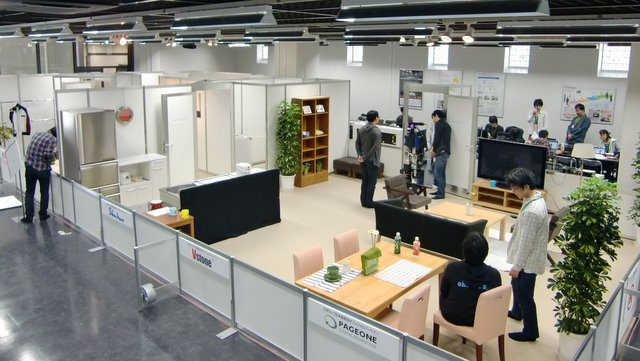
\includegraphics[height=46mm]{images/typical_arena.jpg}} ~ 
  \subfloat[Typical objects]{\label{fig:scenario_objects}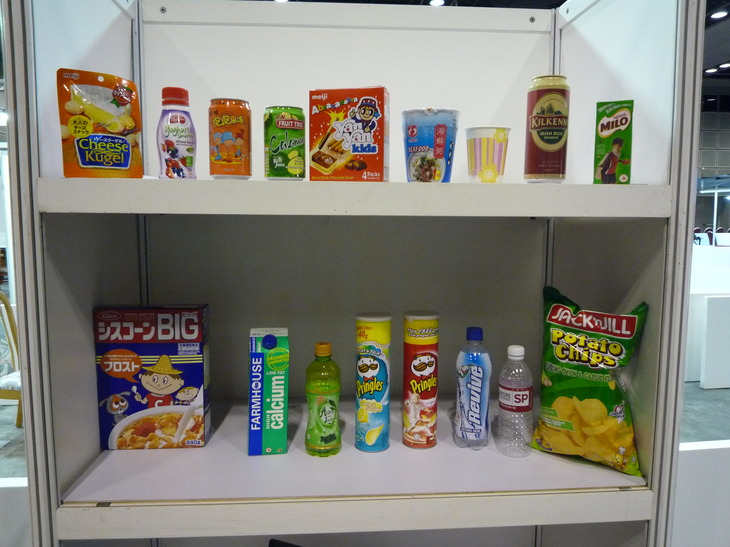
\includegraphics[height=46mm]{images/typical_objects.jpg}}
  \caption{Scenario examples: (a) a typical arena, and (b) typical objects.}
  \label{fig:arena}
\end{figure}



\subsection{Changes to the arena}\label{rule:scenario_changes}

Since the robots should be able to function in the real world the
scenario is not fixed and might change without further notice.
\begin{enumerate}
{\bf\item Major changes:} Changes will primarily influence the position of 
  objects such as furniture inside the arena while walls are likely to stay fixed.
  Multiple changes may take place up to completely restructuring the internals of the apartment. 
  The position of named locations (see \refsec{rule:scenario_names}) are not changed when used in a test, e.g., as navigation goal. \\
  In addition, passages may be blocked and cleared, respectively. 
  One hour before a test slot begins no \iterm{major changes} will be made.
{\bf\item Minor changes:} In contrast to major changes, \iterm{minor changes} like, 
  for instance, slightly moved chairs cannot be avoided and may happen at any time (even during a test). 
\end{enumerate}


\subsection{Predefined objects}\label{rule:scenario_objects}

\def\NumObjects{25\ }
\def\NumLocations{20\ }
\def\NumNames{20\ }

Some tests in the RoboCup@Home league involve the manipulation of objects. 
These objects resemble items usually found in household environments like, for instances, 
soda cans, coffee mugs or books. An example of objects used in a previous competition can be 
seen in \reffig{fig:scenario_objects}.

\begin{enumerate}
{\bf\item Definition:} The TC will compile a list of \NumObjects objects. 
  There are no restrictions on object size, appearance or weight. % (YES, this sentence is NOT NEW, but have been in the old rulebook!) 
  However, it can be expected that the selected objects are easily 
  manipulable by a human using a single hand.
{\bf\item Object classes:} Each object will be assigned to an \iterm{object class}.
  The objects 'lemonade' and 'ice tea' may be of class 'beverage' for example.
{\bf\item Object (class) locations:} Each object (class) will be assigned to an \iterm{object location}.
  Objects of class 'drink' may be usually found on the 'kitchen table' for example. 
{\bf\item Announcement:} The TC makes the set of objects (and their names, classes, and usual locations) available during the setup days.
{\bf\item Known vs.\ unknown}: These objects are used as the \iterm{known objects} in the test specifications;
  \iterm{unknown objects} are not taken from the set of \iterm{predefined objects}. 
{\bf\item Placement:}\nterm{object placement} In manipulation tasks, 
  the objects will be positioned at \iterm{manipulation locations} and less than \SI{15}{\centi\meter} away from the border of the surface 
  they are located at. 
  There will be at least 5cm space around each object.
\end{enumerate}



\subsection{Predefined locations}\label{rule:scenario_locations}

Some tests in the RoboCup@Home league involve \iterm{predefined locations}. 
These may include places like a 'bookshelf' or a 'dining table', as well as certain objects such as a 'television', or the 'front door'. 

\begin{enumerate}
{\bf\item Definition:} The TC will compile a list of predefined locations.
  There are no restrictions on which parts of the arena will be selected as a predefined location. 
{\bf\item Location classes:} Each location will be assigned to a \iterm{location class}. 
  The objects 'couch' and 'arm chair' may be of class 'seat' for example. 
{\bf\item Announcement:} The TC makes the set of locations (and their names and classes) available during the setup days.
{\bf\item Position:} The positions of locations are \emph{not} necessarily fixed (see \refsec{rule:scenario_changes}).
{\bf\item Manipulation locations:} The TC will mark \NumLocations locations out of the set of predefined locations as being \iterm{manipulation locations}.
Whenever a test involves manipulation, the object to manipulate will be placed 
at one of the manipulation locations. 
\end{enumerate}



\subsection{Predefined rooms}\label{rule:scenario_rooms}
Some tests in the RoboCup@Home league involve \iterm{predefined rooms}. 
\begin{enumerate}
{\bf\item Definition:} The TC will compile a list of room names.
{\bf\item Announcement:} The TC makes the set of rooms available during the setup days.
\end{enumerate}



\subsection{Predefined (person) names}\label{rule:scenario_names}

Some tests in the RoboCup@Home league involve \iterm{predefined names} of people. 

\begin{enumerate}
{\bf\item Definition:} The TC will compile a list of \NumNames predefined names.
  The names are \SI{50}{\percent} male and \SI{50}{\percent} female,
  and taken from the (current) most common first names in the United States.\\
  In order to ease speech recognition, it is tried to select names to be phonetically different from each other. 
{\bf\item Announcement:} The TC makes the set of names available during the setup days.
{\bf\item Assignment:} When a test involves interacting with persons (using a person's name),
  all involved persons are assigned names by the referees before the test. 
\end{enumerate}

Typical names are, for example, James, John, Robert, Michael and William as male names;
Mary, Patricia, Linda, Barbara and Elizabeth as female names.


%% %%%%%%%%%%%%%%%%%%%%%%%%
\subsection{Wireless network}\label{rule:scenario_wifi}

For wireless communication, an \iterm{arena network} is provided.
The actual infrastructure depends on the local organization. 

\begin{itemize}
\item To avoid interference with other leagues, this WIFI has to be used for communication only. 
  It is not allowed to use the above or any other WIFI network for personal use at the venue.
\item During the competitions, only the active team is allowed to use the \iterm{arena network}. 
\item The organizers cannot guarantee reliability and performance of wireless communication. 
Therefore, teams are required to be ready to setup, start their robots and run the tests even if, for any reason, network is not working properly.
\end{itemize}

% Preferably the organizers will try to provide one LAN cable on the
% desk of each participating team for Internet connection. However, this
% cannot be guaranteed. If multiple LAN connections are needed, each
% team has to bring its own LAN hub/switch and cables.

\subsection{Smart Home Devices}\label{rule:smarthomedevices}

\todo{Finish writing this section.}
There is a list of official devices that can be used in some tests for additional score.
The protocol to communicate with these devices will be provided well beforehand the
competition.


%%%%%%%%%%%%%%%%%%%%%%%%%%%%%%%%%%%%%%%%%%%%%%%%%%%%%%%%%%%%%%%%%%%%%%%%%%%%%%%
\section{Robots}\label{rule:robots}

\subsection{Autonomy \& Mobility}
Robots that participate in the RoboCup@Home league need to be
\Term{autonomous}{Autonomy} and \Term{mobile}{Mobility}.
Any deviations reported to the TC, may result in a penalty for the team (see \refsec{rule:extraordinary_penalties}).


\subsection{Number of robots}\label{rule:robots_number}

\begin{enumerate}
{\bf\item Registration:} The maximum \term{number of robots} per team that can be registered for the competitions is \emph{two} (2).
{\bf\item Regular Tests:} Only one robot is allowed per test. 
  For different tests different robots can be used.
{\bf\item Open Demonstrations:} In the Open Challenge and the Finals both robots can be used simultaneously.
{\bf\item RoboZoo:} In the RoboZoo both robots can be used simultaneously as long as they fit into the cage.
\end{enumerate}


\subsection{Size and weight of robots}\label{rule:robots_size}

\begin{enumerate}
{\bf\item Dimensions:} The dimensions of a robot should not exceed the limits of an average door, 
which is \SI{200}{\centi\meter} by \SI{70}{\centi\meter} in most countries.\\ 
The TC may allow the qualification and registration of larger robots, 
but due to the international character of the competition it cannot be guaranteed that the robots can actually enter the arena.  
In case of doubt, contact the local organization. 
{\bf\item Weight:} There is no specific weight restriction. 
However, the weight of the robot and the pressure it exerts on the floor should not exceed 
local regulations for the construction of buildings which are used for
living and/or offices in the country where the competitions is being held.
{\bf\item Transportation:} Team members are responsible for quickly moving the robot out of the arena. 
If the robot cannot move by itself (for any reason), the team members must 
be able to transport the robot away with an easy and fast procedure.
\end{enumerate}



\subsection{Emergency stop button}\label{rule:robots_emergency_button}

\begin{enumerate}
{\bf\item Accessibility and visibility:} Every robot has to provide an easily accessible and visible \iterm{emergency stop} button. 
{\bf\item Color:} It must be coloured red, and preferably be the only red button on the robot. 
If it is not the only red button, the TC may ask the team to tape over or remove the other red button. 
{\bf\item Robot behavior:} When pressing this button, the robot and all parts of it have to stop moving immediately.
{\bf\item Inspection:} The emergency stop button is tested during the \iterm{Robot Inspection} test (see \refsec{sec_robot_inspection}).
\end{enumerate}



\subsection{Start button}
\label{rule:start_button}

\begin{enumerate}
  {\bf\item Requirements:} As stated in \refsec{rule:start_signal}, teams that aren't able to carry out the default start signal (opening the door) have to provide a \iterm{start button} that can be used to start tests. The team needs to announce this to the TC before every test that involves a start signal, including \iterm{Robot Inspection}.
  {\bf\item Definition:} The start button can be any ``one-button procedure'' that can be easily executed by a referee.  This includes, for example, the release of the \iterm{emergency button} (\refsec{rule:robots_emergency_button}), a hardware button different from the \iterm{emergency button} (e.g., a green button), or a software button in a Graphical User Interface. 
  {\bf\item Inspection:} It is during the the \iterm{Robot Inspection} test (see \refsec{sec_robot_inspection}) that the procedure for the start button, if needed, is announced to the TC and inspected. The start button for a robot should be the same for all the tests.
  {\bf\item Penalty for using start button:} If a team needs to use the start button in a test where opening the door is the start signal, it may receive a penalty (see \refsec{rule:start_signal}).
\end{enumerate}



\subsection{Appearance and safety}\label{rule:roobt_appearance}

Robots should have a nice product-like appearance, be safe to operate and should not annoy its human users.
The following rules apply to all robots and are part of the \iterm{Robot Inspection} test (see \refsec{sec_robot_inspection}). 
\begin{enumerate}
{\bf\item Cover:} The robot's internal hardware (electronics and cables) should be covered in an appealing way.
The use of (visible) duct tape is strictly prohibited.
{\bf\item Loose cables:} There may not be any loose cables hanging out of the robot. 
{\bf\item Safety:} The robot may not have sharp edges or other things that could severe people.
{\bf\item Annoyance:} The robot should not permanently make loud noises or use blinding lights.
\end{enumerate}




\subsection{Audio output plug}\label{rule:roobt_audio_out}

\begin{enumerate}
{\bf\item Mandatory plug:} Either the robot or some external device connected to it \emph{must} have a \iterm{speaker output plug}. 
It is used to connect the robot to the sound system so that the audience and the referees can hear and follow the robot's speech output.
{\bf\item Inspection:} The output plug needs to be presented to the TC during the \iterm{Robot Inspection} test (see \refsec{sec_robot_inspection}).
{\bf\item Audio during tests:} Audio (and speech) output of the robot during a test have to be understood at least by the referees and the operators.
\begin{compactitem}
\item It is the responsibility of the teams to plug in the transmitter before a test, 
to check the sound system, 
and to hand over the transmitter to next team.
\item Do not rely on the sound system! 
For fail-safe operation and interacting with operators make sure that the sound system is not needed, e.g., 
by having additional speakers directly on the robot.
\end{compactitem}
\end{enumerate}

\section{External devices}\label{rule:roobt_external_devices}
\begin{enumerate}
{\bf\item Definition:} Everything which is not part of the robot is considered an \iterm{external device}. 
{\bf\item Inspection:} In general, external devices are not allowed unless presented and explained to the Technical Committee during the \iterm{Robot Inspection} test (see \refsec{sec_robot_inspection}).
{\bf\item Supervision:} In regular tests, external devices may only be used under supervision by referees and after approval by the TC. The devices have to be brought to the arena for every test, and removed quickly after the test.
{\bf\item Open demonstrations:} For the Open Challenge, RoboZoo, and the finals, external devices are allowed, still their use needs to be announced beforehand.
{\bf\item Wireless devices:} All \iterm{wireless devices} including bluetooth devices, walkie-talkies, and anything else that uses an RF signal to operate need to be announced to the \term{Organizing Committee (OC)}. The use of any wireless device not approved by the TC is strictly prohibited.  
{\bf\item Artificial landmarks:} \iterm{Artificial landmarks} and \iterm{markers} are not allowed.
{\bf\item Computing devices:} External computers for decentralized computations are allowed, but have to be inside the arena, i.e.,~not on its periphery.
{\bf\item Wireless LAN:} The use of networks other than the \iterm{arena network} (see \refsec{rule:scenario_wifi}) is strictly prohibited.
{\bf\item External microphones: }\iterm{External microphones}, hand microphones, and headsets are not allowed. Using an \iterm{on-board microphone} is mandatory for communication with the robot.
\end{enumerate}



\section{Organization of the competition}\label{sec:procedure_during_competition}

\subsection{Stage system}\label{rule:stages}

The competition features a \iterm{stage system}. 
It is organized in two stages each consisting of a number of specific tests. 
It ends with the finals.

\begin{enumerate}
{\bf\item Stage~I:} The first days of the competition will be called \iterm{Stage~I}. 
  All qualified teams can participate in Stage~I.
  Stage~I comprehends a set of \iterm{Ability Tests} and an \iterm{Integration Test}. Those \iterm{Proficency Tests} are performed at least 3 times each one.
  The \iterm{Open Challenge} is the open demonstration in Stage~I.

% MAURICIO: The advance schema changed. Also no demo challenge for 2015
%{\bf\item Stage~II:} The best \emph{50\% of teams}\footnote{If the total number of teams is less than 20, then the best 10 teams advance to Stage~II.} (after Stage~I) advance to \iterm{Stage~II}. 
%  Here, more complex abilities or combinations of abilities are tested. 
%  The \iterm{Demo Challenge} is the open---but scoped---demonstration in Stage~II.
{\bf\item Stage~II:} The best \emph{50\% of teams with full integrated capabilities}\footnote{If the total number of teams is less than 20, up to 10 teams may advance to Stage~II} (after Stage~I) advance to \iterm{Stage~II}. 
  Here, more complex abilities or combinations of abilities are tested. 
  In order to advance to Stage~II a team must successfully solve 3 out of 5 of the \iterm{Proficency Tests} in Stage~I
%  The \iterm{Open Challenge} is the open demonstration in Stage~II.
{\bf\item Final demonstration:} The best \emph{five teams} (after Stage~I and Stage~II) advance to the final round. 
  The final round features only a single open demonstration.
\end{enumerate}
% MAURICIO: No technical challenge for 2015
% In addition, a Technical Challenge (see \refsec{sec:TechnicalChallenge}) is carried out between Stage~II and the Final Demonstration, and its schedule is outside the scope of the Stage system.
In case of having no considerable score deviation between a team advancing to the next stage and a team dropping out, the TC may announce additional teams advancing to the next stage.


\subsection{Number of tests}\label{rule:number_of_tests}

\begin{enumerate}
\item In Stage~I, the \term{maximum number of tests} that a team can participate in is \emph{five (5)}.
\item In Stage~II, the \term{maximum number of tests} that a team can participate in is \emph{four (4)}.
\item None of the tests is mandatory, except for the \iterm{Robot Inspection} test (see \refsec{sec_robot_inspection}), the \iterm{Robo-Zoo} test (see \refsec{test:INTHOME}), and the \iterm{Basic Functionalities} test (see \refsec{test:BFPS}).
\item Teams have to indicate to the organizing committee in which tests they are going to participate. 
  Otherwise, they are automatically added to all test schedules and 
  may receive a penalty when not attending (see \refsec{rule:not_attending}).
\end{enumerate}


\subsection{Schedule}\label{rule:schedule}

\begin{enumerate}
{\bf\item Tests:} The organizing committee (OC) provides schedules for all tests and teams. 
{\bf\item Slots:} The tests will be held in \iterm{test slots} of approximately two hours.  
{\bf\item Preparation:} The organizing committee (OC) provides schedules for all teams to organize the access to the arena between test slots.
In these \iterm{preparation slots} the teams may conduct calibration procedures, remap the arena if necessary, or conduct test runs.
Preparation slots are inserted whenever possible, but may not be available before all test slots. 
{\bf\item Arena access:} One hour before a test slot, only the teams participating in that slot are allowed in the arena.
This rule only applies when not having organized \iterm{preparation slots}.   
\end{enumerate}


%\subsection{Score system}\label{rule:score_system}
%
%\begin{enumerate}
%  {\bf\item Stage~I:} The maximum total score per test in Stage~I is \scoring{2000 points}.
%  {\bf\item Stage~II:} The maximum total score per test in Stage~II is \scoring{2600 points}.
%  {\bf\item Special tests:} Tests may specify a maximum total score deviating from the general maximum total scores.  
%  {\bf\item Minimum score:} The minimum total score per test in Stage~I and Stage~II is \scoring{0 points}. 
%  That is, if the total score for a test is below zero, the team does not receive any points.
%  {\bf\item Penalties:} An exception to the \emph{minimum score} rule are penalties. 
%  Both penalties for not attending (see \refsec{rule:not_attending}) and extraordinary 
%  penalties (see \refsec{rule:extraordinary_penalties}) can cause a total negative score. 
%  {\bf\item Partial scores:} All tests---except for the open demonstrations---are rewarded on a partial scoring basis. 
%  \begin{enumerate}
%  \item Tests are split into designated parts.
%  \item Each part is assigned a certain number of points.
%  \item A team that successfully passes a designated part of the test receives points for that part.
%  \item In case of partial success, referees (and TC members) may decide to only award a percentage instead of the full partial score.  
%  \item The total score for a test is the sum of partial scores.
%  \item Partial scores can be negative (e.g.~to penalize failures etc.).
%  \end{enumerate}
%\end{enumerate}

% MAURICIO: Explained Score System
\subsection{Score system}\label{rule:score_system}

\begin{enumerate}
  {\bf\item Stage~I:} The maximum total score in Stage~I is \scoring{100 points}.
  \begin{enumerate}
    {\bf\item \iterm{Proficency Tests}:} The maximum total score is calculated as the average of the best two runs for that test
    {\bf\item RoboZoo:} The maximum score for RoboZoo is \scoring{5 points}.
  \end{enumerate}
  
  {\bf\item Stage~II:} Test in Stage~II are rewarded on a task-solved scoring basis.
  \begin{enumerate}
  \item Each test but the Open Challenge has a main task. The base score for solving the main task is \scoring{25 points}.
  \item The maximum score for Open Challenge is \scoring{20 points}.
  \item Optionals and subtasks add bonus points to the main task score.
  \end{enumerate}

  {\bf\item Finals:} Final score is normalized and special evaluation is used

  {\bf\item Special tests:} Tests may specify a maximum total score deviating from the general maximum total scores.
  {\bf\item Minimum score:} The minimum total score per test in Stage~I and Stage~II is \scoring{0 points}. That is, if the total score for a test is below zero, the team does not receive any points.
  {\bf\item Penalties:} An exception to the \emph{minimum score} rule are penalties. Both penalties for not attending (see \refsec{rule:not_attending}) and extraordinary penalties (see \refsec{rule:extraordinary_penalties}) can cause a total negative score. 
  {\bf\item Partial scores:} All tests---except for the open demonstrations---are rewarded on a partial scoring basis. 
  \begin{enumerate}
  \item Tests are split into designated parts.
  \item Each part is assigned a certain number of points.
  \item A team that successfully passes a designated part of the test receives points for that part.
  \item In case of partial success, referees (and TC members) may decide to only award a percentage instead of the full partial score.  
  \item The total score for a test is the sum of partial scores.
  \item Partial scores can be negative (e.g.~to penalize failures etc.).
  \end{enumerate}
\end{enumerate}


% MAURICIO: On 2015, Open Challenge may be moved to Stage 2. There is no Demo Challenge
\subsection{Open Demonstrations} \label{sec:open-demonstrations}
\begin{enumerate}
  {\bf\item Stage~I:} The \iterm{Open Challenge} is the open demonstration in Stage~I.
  \begin{enumerate}
  \item To participate in the Open Challenge, a team needs to participate in at least one regular Stage~I test.
  \item Teams can demonstrate freely chosen abilities. 
  \item The performance is evaluated by a jury consisting of the team leaders of all other teams.
  \item The Open Challenge is described in \refsec{sec:test_open_challenge}.
  \end{enumerate}
%  {\bf\item Stage~II:} The \iterm{Demo Challenge} is the open demonstration in Stage~II.
%  \begin{enumerate}
%  \item To participate in the Demo Challenge, a team needs to participate in at least one regular Stage~II test.
%  \item The scope (and topic) of the Demo Challenge are defined by the TC on a yearly basis.
%  \item Teams can demonstrate freely chosen abilities, but according to the scope. 
%  \item The performance is evaluated by the Technical Committee.
%  \item The Demo Challenge is described in \refsec{sec:test_demo_challenge}.
%  \end{enumerate}
  {\bf\item Finals:} The competition ends with a final demonstration.
  \begin{enumerate}
  \item The concept of the final demonstration is the same as that of the Open Challenge, but the performance evaluation is different. 
  \item The are two juries---an \emph{external} consisting of three or more people not from the RoboCup @Home league, and an \emph{internal} formed by the Executive Committee. Both juries have different sets of evaluation criteria.
  \item Members of the external jury are selected by the Executive Committee on site. 
  \item The demonstration in the finals does not have to be different from the one shown in the Open Challenge. It does not have to be the same either.
  \end{enumerate}
\end{enumerate}


\section{Procedure during Tests}

\subsection{Safety First!}\label{rule:safetyfirst}
\begin{enumerate}
{\bf\item Emergency Stop:} At any time when operating the robot inside and outside the 
  scenario the owners have to stop the robot immediately if there is a remote possibility 
  of dangerous behavior towards people and/or objects. 
{\bf\item Stopping on request:} If a referee, member of the Technical or Organizational 
  committee, an Executive or Trustee of the federation tells the team to stop the robot, 
  there will be no discussion and the robot has to be stopped \emph{immediately}.
{\bf\item Penalties:} If the team does not comply, the team and its members can be excluded 
  from the ongoing competition immediately by a decision of the RoboCup@Home Technical Committee. 
  Furthermore, the team and its members can be banned from future competitions for a period 
  not less than a year by a decision of the RoboCup Federation Trustee Board.
\end{enumerate}



\subsection{Maximum number of team members}\label{rule:number_of_people}
\begin{enumerate}
  {\bf\item Regular Tests:} During a regular test, the maximum number of team members allowed inside the arena is \emph{one} (1).
    The only exceptions are tests that require for more team members in the arena.
  {\bf\item Setup:} During the setup of a test, 
    the number of team members inside the arena is not limited. 
  {\bf\item Open Demonstrations:} During the Open Challenge, and the final demonstration, 
    the number of team members inside the arena is not limited. 
  {\bf\item Moderation:} During a regular test, one team member \emph{must} be available to host and comment the event (see \refsec{rule:moderator}).
\end{enumerate}



\subsection{Fair play}\label{rule:fairplay}
\iterm{Fair Play} and cooperative behavior is expected from all teams during the entire competition, in particular:
\begin{itemize}
\item while evaluating other teams, 
\item while refereeing, and 
\item when having to interact with other teams' robots.  
\end{itemize}
This also includes:
\begin{itemize}
\item not trying to cheat (e.g.~pretending autonomous behavior where there is none), 
\item not trying to exploit the rules (e.g.~not trying to solve the task but trying to score), and 
\item not trying to make other robots fail on purpose. 
\end{itemize}
Disregard of this rule can lead to penalties in the form of negative scores, and disqualification 
for a test or even for the entire competition. 

\subsection{Robot Autonomy and Remote Control}
\begin{enumerate}
{\bf\item No touching:} During a test, the participants are not allowed to make contact with the robot(s), 
  unless it is in a ``natural'' way and/or required by the test specification. 
{\bf\item Natural interaction:} The only allowed means to interact with the robot(s) are gestures and speech.
{\bf\item Natural commands:} Only general instructions are allowed. 
Anything that resembles direct control is prohibited.
 
{\bf\item Remote Control:} Remotely controlling the robot(s) is strictly prohibited. 
This also includes pressing buttons, or influencing sensors on purpose.
{\bf\item Penalties:} Disregard of these rules can lead to penalties in the form of negative scores, and disqualification 
for a test or even for the entire competition. 
\end{enumerate}

\subsection{Collisions}
\begin{enumerate}
  {\bf\item \iterm{Touching}:} Robots are allowed to gently \emph{touch} objects, items and humans. 
  They are not allowed to crash into something. 
  The "safety first" rule (\refsec{rule:safetyfirst}) supercedes all other rules.
  \begin{itemize}
   \item It \emph{is} allowed however to \emph{functionally} touch an item with e.g. the base.
  \end{itemize}
  The OC/TC/EC and the RoboCup Trustees all have the right to immediately stop a robot, and to disqualify a team for the 
  duration of the competition, or longer, in case of \emph{dangerous} behavior. 
  Furthermore, referees can recommend to disqualify a team in which case EC/TC decides.
  {\bf\item \iterm{Major collisions}:} If a robot crushes into something during a test, the robot is immediately stopped.
  Additional penalties may apply. 
  {\bf\item Robot-Robot avoidance:} If two robots encounter each other, they both have to actively try to avoid the other robot.
  \begin{enumerate}
  \item A robot which is not going for a different route 
    within a reasonable amount of time (e.g., \SI{30}{\second}) is removed.
  \item A non-moving robot blocking the path of another robot 
    for longer than a reasonable amount of time (e.g., \SI{30}{\second}) is removed.
    In this context, ``moving'' refers to any kind of motion or action required in the test. 
    For example, a robot standing still but manipulating an object does 
    not need to stop manipulating and move away, even when blocking the way
    of another robot for the duration of the manipulation.
  \end{enumerate}
\end{enumerate}



\subsection{Removal of robots}\label{rule:robot_removal}
Robots not obeying the rules are stopped and removed from the arena.
\begin{enumerate}
\item It is the decision of the referees and the TC member monitoring the test if and when to remove a robot.
\item When told to do so by the referees or the TC member monitoring the test, the team has to immediately stop the robot,
  and remove it from the arena without disturbing the ongoing test.
\end{enumerate}


\subsection{Start signal}\label{rule:start_signal}

\begin{enumerate}
  {\bf\item Opening the door:} Unless stated otherwise, the cue for the robot to enter the arena and start the test is the opening of the door by a referee.
  {\bf\item Start button:} If the robot is not able to automatically start after opening the door, the team may start the robot using a start button. 
  \begin{enumerate}
    \item Using a start button needs to be announced to the referees. It is the responsibility of the team to do so before the test starts.
    \item There may be penalties for using a start button in some tests
  \end{enumerate}
\end{enumerate}


\subsection{Entering and leaving the arena}\label{rule:start_position}
\begin{enumerate}
  {\bf\item Start position:} Unless stated otherwise, the robot starts outside of the arena.
  {\bf\item Entering:} The robot has to autonomously enter the arena.
  {\bf\item Success:} The robot is said to \emph{have entered} when the door used to enter can be closed again, and the robot is not blocking the passage.
\end{enumerate}



\subsection{Gestures}\label{rule:gestures}
Hand gestures may be used to control the robot in the following way:
\begin{enumerate}
{\bf\item Definition:} The teams define the hand gestures by themselves. 
{\bf\item Approval:} Gestures need to be approved by the referees and TC member monitoring the test.
Gestures should not involve more than the movement of both arms. 
This includes e.g.~expressions of sign language or pointing gestures.
{\bf\item Instructing operators:} It is the responsibility of the team to instruct operators.
\begin{enumerate}
\item The team may only instruct the operator when told to so by a referee.
\item The team may only instruct the operator in the presence of a referee.
\item The team may only instruct the robot for as long as allowed by the referee.
\item When the robot has to instruct the operator, it is the robot that instructs the operator and \emph{not} the team.
The team is not allowed to additionally guide the operator, e.g., tell the operator to come closer, speak louder, or to repeat a command.
\end{enumerate}
{\bf\item Receiving gestures:} Unless stated otherwise, it is not allowed to use 
a speech command to set the robot into a special mode for receiving gestures.
\end{enumerate}



\subsection{Referees}\label{rule:referees}
% \refmark{}
\begin{enumerate}
{\bf\item Setup:} Unless stated otherwise, each test is monitored by two referees and one member of the Technical Committee.
{\bf\item Selection:} The two referees 
\begin{itemize}
\item are chosen by EC/TC/OC, 
\item are announced together with the schedule for the test slot, 
\item and have to referee all teams in that slot.
\item Referees may not be from one of the teams in the slot.
\end{itemize}
{\bf\item Not showing up:} Not showing up for refereeing (on time) will result in a penalty (see \refsec{rule:extraordinary_penalties}). 
{\bf\item TC monitoring:} The referee from the TC acts as a main referee. 
{\bf\item Referee instructions:} Right before each test, referee instructions are conducted by the TC. The referees for all slots need to be present at the arena where the referee instructions are taking place.When and where referee instructions are taking place is announced together with the schedule for the slots.
\end{enumerate}


\subsection{Operator}\label{rule:operator}
\begin{enumerate}
{\bf\item Default operator:} The robots are operated by the monitoring TC member, 
a referee, or by a person selected by the TC.
{\bf\item Fallback/custom operator:} If the robot fails to understand the command given by the default operator, the team may continue with a custom operator.
\begin{compactitem}
\item The custom operator may be any person chosen by the team (and willing to do so); 
  including the referees or the monitoring TC member. 
\item A penalty may be involved when using a custom operator.
\end{compactitem}
\end{enumerate}

\subsection{Moderator}\label{rule:moderator}
\begin{enumerate}
{\bf\item Providing a moderator:} For each regular test (i.e., not for the open demonstrations), 
all participating teams need to provide a team member as moderator for the duration of their performance. 
{\bf\item Responsibilities:} The moderators have to:
  \begin{compactitem}
  \item explain the rules of the test, 
  \item comment on the performance of their team, 
  \item not interfere with the performance, 
  \item speak in English, 
  \item and obey the instructions by the monitoring TC member.
  \end{compactitem}
{\bf\item Competitive tests:} In competitive tests (tests in which two teams directly compete against each other),
the moderation has to be done by the two teams together.
\end{enumerate}


\subsection{Time limits}\label{rule:time_limits}
\begin{enumerate}
{\bf\item Stage~I:} Unless stated otherwise, the time limit for each test in Stage~I is \timing{5 minutes}.
{\bf\item Stage~II:} Unless stated otherwise, the time limit for each test in Stage~II is \timing{10 minutes}.
{\bf\item Setup time:} Unless stated otherwise, all time specifications, e.g., setup time and time for instructing operators, 
 are within the total test time. 
{\bf\item Scores:} When the time is up, the team has to immediately remove their robot(s) from the arena; no more points can be scored.
In special cases, the monitoring TC member may ask the team to continue the test for demonstration purposes (points cannot be scored). 
\end{enumerate}



\subsection{Restart}\label{rule:restart}
\begin{enumerate}
{\bf\item Number of restarts:} A team may request one (1) restart during a test, unless stated in otherwise.
There are tests in which a restart is not allowed.
{\bf\item Procedure:} In case a restart is allowed, the team may request the restart only before 50\% of the time alloted to the test.
The complete test is then restarted from the beginning (e.g., with entering the arena).  
The referees may rearrange the locations of objects/persons if necessary.
{\bf\item Time:} The time is neither restarted nor stopped. The team has 1 minute to restart the test (the same time to start the test); if the team is not able to do so in the allotted time, the test is called as finished by the TC.
{\bf\item Score:} The score of the second run (after the restart) counts. 
If it is lower than the score of the first run (before the restart),  
the average score of first and second run is taken.
{\bf\item Forced restart:} The referees and the monitoring TC member may force the team to do a restart:
\begin{compactitem}
  \item if the robot is doing nothing or nothing reasonable for \timing{one minute}, or
  \item when the robot fails to understand a command for \timing{five times}.
\end{compactitem}  
\end{enumerate}


\subsection{Bypassing Automatic Speech Recognition: Continue}\label{rule:asrcontinue}

Giving commands to the robot is an important part of many tests.
RoboCup@Home fosters natural human-robot interaction through gestures and speech, such that speech is the primary modality to give complex commands to the robot.
Due to the sequential nature of many tests and the difficulty of ASR in the international competition environment of RoboCup,
the team is allowed to take up to 2 alternative means to provide a command to the robot, for which the robot continuously fails to recognize the spoken command.
These alternative means should be declared in the registration form and checked by the TC during the \iterm{Robot Inspection} test (see \refsec{sec_robot_inspection}).

In future competitions, this rule will be gradually removed. 
Hence, solutions are encouraged that either resolve the ASR failure through spoken dialogues or solving the task in an alternative way (no penalty), or that use appealing modalities to provide the command (less penalty than direct typing on the robot).

\begin{enumerate}
{\bf\item Number of Continue's:} The team leader may request up to two (2) Continue's during a test. 
{\bf\item Procedure:} In case a Continue is allowed, the team may request the Continue only at moments in which the robot is failing at carrying out ASR (no pre-emptive Continue's are allowed).
A TC member gives the command through the alternative input modality. S/he provides exactly what the user has spoken. 
The Continue rule will not be allowed, if the robot does not have a keyboard attached or the alternative input modality was not accepted by the TC, or if it is not able to process ASR commands and alternative commands simultaneously.
{\bf\item Time:} The time is neither restarted nor stopped while the Continue rule is applied.
{\bf\item Score:} If one Continue was asked for, the points provided for the ASR part of the test (if any) will be zero and the total points for the test will be multiplied by a factor of 0.5 if the modality of the alternative solution is by typing on a keyboard. To promote other means of interaction, if the modality is different than keyboard typing (i.e. touch interface), the factor to be applied will be 0.75. If two Continues were asked for, the factor will be applied twice.
\end{enumerate}

\subsubsection{Alternative methods}
Below are some suggested alternatives for ASR:
\begin{itemize}
 \item A QR code encoding a text is shown to the robot on a laptop screen.
 \item The robot hosts a website on which some text can be entered.
 \item A laptop connects to the robot over e.g. ssh where some command can be entered. 
 \item ...
\end{itemize}




\section{Special penalties and bonuses}\label{sec:special_awards}


\subsection{Penalty for not attending}\label{rule:not_attending}
\begin{enumerate}
{\bf\item Automatic schedule:} All teams are automatically scheduled for all tests.
{\bf\item Announcement:} If a team cannot participate in a test (for any reason),
the team leader has to announce this to the OC at least \timing{60 minutes} before the test slot begins.
{\bf\item Penalties:} A team that is not present at the start position when their scheduled test starts, the team is not allowed to participate in the test anymore. If the team has not announced that it is not going to participate, it gets a penalty of \scoring{500 points}. 
\end{enumerate}

\subsection{Extraordinary penalties}\label{rule:extraordinary_penalties}
\begin{enumerate}
{\bf\item Penalty for inoperative robots:} If a team starts a test, but it does not solve any of the partial tasks
(and is obviously not trying to do so), a penalty of \scoring{-100 points} is handed out. 
The decision is made by the referees and the monitoring TC member.  
{\bf\item Extra penalty for collision:} In case of major, (grossly) negligent collisions the TC may disqualify the team for 
a test (the team receives \scoring{0 points}), or for the entire competition.
{\bf\item Not showing up as referee or jury member:}
If a team does not provide a referee or jury member (being at the arena on time), the team receives a penalty
of \scoring{500 points}, and will be remembered for qualification decisions in future competitions.\\
Jury members missing a performance to evaluate are excluded from the jury, and the team is 
disqualified from the challenge (receives \scoring{0 points}).
\end{enumerate}

\subsection{Bonus for outstanding performance}\label{rule:outstanding_performance}
\begin{enumerate}
\item For every regular test in Stage~I and Stage~II, the @Home Technical
Committee can decide to give an extra bonus for \iterm{outstanding performance} 
of up to 10\% of the maximum test score. 
\item This is to reward teams that do more than what is needed to solely score points in a
test but show innovative and general approaches to enhance the scope of @Home. 
\item If a team thinks that it deserves this bonus, it should announce (and briefly explain) 
this to the Technical Committee beforehand.
\item It is the decision of the TC if (and to which degree) the bonus score is granted.
\end{enumerate}


\section{Best Test Score Certificate}\label{sec:best_score_certificate}
A certificate will be given to the team with the highest score in each test of Stage 1 and 2. 

\begin{enumerate}
{\bf\item Requirements:} The score obtained must be at least 70\% of the maximum score of the test.
\end{enumerate}
% Local Variables:
% TeX-master: "../../rulebook"
% End:

\section{General Instructions for Organizing Committee}\label{sec:oc_general_instructions}
Although there are instructions for the OC are specified per test, there are several aspects that the OC requires to carry out for competition in general:
\begin{description}
\item[During competition:] \hfill
\begin{compactitem}
\item Provide TC and referees with scoring sheets, pens, clipboards, stopwatches and other material relevant of carrying out the scoring.
\item Post time schedules in the allotted spaces for the team's knowledge.
\end{compactitem}
\item[1h before each test:] \hfill
\begin{compactitem}
\item Organize referees.
\end{compactitem}
\end{description}




\chapter{Setup and Preparation}
\label{chap:setup_and_preparation}
Prior to the RoboCup@Home competition, all arriving teams will have the opportunity to setup their robots and prepare for the competition in a \iterm{Setup \& Preparation} phase. This phase is scheduled to start on the first day of the competition, i.e., when the venue opens and the teams arrive. During the setup phase, teams can assemble and test their robots. On the last setup day, a \iterm{welcome reception} will be held. To foster the knowledge exchange between teams a conference-like \iterm{poster session} takes place during the reception. All teams have to get their robots inspected by members of the TC to be allowed to participate in the competition.

\paragraph{Regular tests are not conducted during setup \& preparation.} The competition starts with Stage~I ( Section \refsec{chap:stage_I}).

\begin{table}[h]
  \newcolumntype{C}[1]{>{\centering\let\newline\\\arraybackslash\hspace{0pt}}m{#1}}
  \newcolumntype{S}{C{1.6cm}}
  \newcolumntype{M}{C{3.2cm}}
  \begin{center}
    \caption{Stage System and Schedule (distribution of tests and stages over days may vary)}
    \begin{tabularx}{14.56cm}{S|S|S|S|S|S|S|S}
      \hline
      \multicolumn{2}{|M|}{ \cellcolor[HTML]{FFFFC7}Setup \& \newline Preparation} &
      \multicolumn{2}{M|}{ \cellcolor[HTML]{67FD9A}\iterm{Stage~I}} &
      \multicolumn{2}{M|}{ \cellcolor[HTML]{9698ED}\iterm{Stage~II}} &
      \multicolumn{2}{M|}{ \cellcolor[HTML]{FFCCC9}\iterm{Finals}}\\
      \hline
      %Second row
      \multicolumn{1}{S|}{} &
      \multicolumn{2}{M|}{$\xrightarrow{advance}$\newline All teams that \newline passed Inspection} &
      \multicolumn{2}{M|}{$\xrightarrow{advance}$\newline Best 10 ($<20$) \newline or best 50\% ($\geq 20$)} &
      \multicolumn{2}{M|}{$\xrightarrow{advance}$\newline Best 5 \newline teams} &
      \multicolumn{1}{C{1.2cm}}{~}
      \\ \cline{2-7}
    \end{tabularx}
  \end{center}
\end{table}


\section{General Setup}
\label{sec:general_setup}
Depending on the schedule, the \iterm{Setup \& Preparation} phase lasts for one or two days.

\begin{enumerate}
	\item \textbf{Start:} Setup \& Preparation starts when the venue opens for the first time.
	\item \textbf{Intention:} During Setup \& Preparation, teams arrive, bring or receive their robots, and assemble and test them.
	\item \textbf{Tables:} The local organization will setup and randomly assign team tables.
	\item \textbf{Groups:} Depending on the number of teams, the \iaterm{Organizing Committee}{OC} may form multiple groups of teams (usually two) for the first (and second stage). The OC will assign teams to groups and announce the assignment to the teams.
	\item \textbf{Arena:} The arena is available to all teams during Setup \& Preparation. The OC may schedule special test or mapping slots in which arena access is limited to one or more teams exclusively (all teams get slots). Note, however, that the arena may not yet be complete and that last works are conducted in the arena during the setup days.
	\item \textbf{Objects:} The delegation of EC, TC, OC and local organizers will buy the objects (see Section \refsec{rule:scenario_objects}). Note, however, that the objects may not be available at all times and not from the beginning of Setup \& Preparation.
\end{enumerate}

\section{Welcome Reception}
\label{sec:welcome_reception}
Traditionally --since Eindhoven 2013-- the RoboCup@Home holds an own \iterm{welcome reception} in addition to the official opening ceremony. During the welcome reception, a \iterm{poster session} is held in which teams present their research foci and latest results (see Section \refsec{sec:poster_teaser_session}).
\begin{enumerate}
	\item \textbf{Time:} The welcome reception is held in the evening of the last setup day.
	\item \textbf{Place:} The welcome reception takes place in the @Home arena and/or in the RoboCup@Home team area.
	\item \textbf{Snacks \& drinks:} During the welcome reception snacks and beverages (beers, sodas, etc.) are served.
	\item \textbf{Organization:} It is the responsibility of the OC and the local organizers to organize the welcome reception \& poster session including
		\begin{enumerate}
			\item organizing poster stands (one per team) or alternative to present the posters,
			\item organizing the snacks and drinks,
			\item inviting officials, sponsors, local organization and the trustees of the RoboCup Federation to the event.
		\end{enumerate}
	\item \textbf{Poster presentation:} During the welcome reception, the teams give a poster presentation on their research focus, recent results, and their scientific contribution.
	Both the poster and the teaser talk are evaluated by a jury (see \ref{sec:poster_teaser_session}).
\end{enumerate}

\section{Poster Teaser Session}
\label{sec:poster_teaser_session}
Before the welcome reception \& poster session, a \iterm{poster teaser session} is held. In this teaser session, each team can give a short presentation of their research and the poster being presented at the poster session.

\subsection{Poster teaser session}
\begin{enumerate}
	\item \textbf{Presentation:} Each team has a maximum of three minutes to give a short presentation of their poster.
	\item \textbf{Time:} The poster teaser session is to be held before the welcome reception \& poster session (see Section \refsec{sec:welcome_reception}).
	\item \textbf{Place:} The poster session may be held in or around the arena, but should not interfere with the robot inspection (see Section \refsec{sec:robot_inspection}).
	\item \textbf{Evaluation:} The teaser presentation and the poster presentation are evaluated by a jury consisting of members of the other teams. Each team has to provide one person (preferably the team-leader) to follow
	and evaluate
	the entire poster teaser session and the poster session. Not providing a person results in no score for this team in the \iterm{Open Challenge}.

	%%%%%%%%%%%%%%%%%%%%%%%%%%%%%%%%%%%%%%%%%%%%%%%%%%%%%%%%%%%%%%%%%%%%%%%%%%%%%%
	%
	% In previous years, scores from teaser session has not been used for scoring
	% during competition. Therefore, this section has been commented out
	%
	%%%%%%%%%%%%%%%%%%%%%%%%%%%%%%%%%%%%%%%%%%%%%%%%%%%%%%%%%%%%%%%%%%%%%%%%%%%%%%
	\item \textbf{Criteria:} For each of the following evaluation criteria, a maximum of 10 points is given per jury member:
	\begin{enumerate}
		\item Novelty and scientific contribution
		\item Relevance for RoboCup@Home
		\item Presentation (Quality of poster, teaser talk and discussion during poster session)
	\end{enumerate}
	\item \textbf{Score:} The points given by each jury member are scaled to obtain a maximum of 50 points. The total score for each team is the mean of the jury member scores. To neglect outliers, the N best and worst scores are left out:
	$$
	score=\frac{\sum \text{team-leader-score}}{\text{number-of-teams}-\left ( 2N+1  \right )},N=\left\{\begin{matrix}
	1, & \text{number-of-teams} \geq 10\\ 
	2, & \text{number-of-teams} < 10
	\end{matrix}\right.
	$$
	\item \textbf{Sheet collection:} Evaluation sheets are collected by the OC at a later time (announced beforehand by the OC), allowing teams to continue knowledge exchange during the first days of the competition (Stage~I).
	\item \textbf{OC Instructions:}
	\begin{itemize}
		\item Prepare and distribute evaluation sheets (before the poster teaser session.)
		\item Collect evaluation sheets.
		\item Organize and manage the poster teaser presentations and the poster session.
	\end{itemize}
\end{enumerate}

\section{Robot Inspection}
\label{sec:robot_inspection}
Safety is the most important issue when interacting with humans and operating in the same physical workspace. Because of that all participating robots are inspected before participating in RoboCup@Home. Every team needs to get its robot(s) inspected and approved for participation.

\begin{enumerate}
	\item \textbf{Procedure:} The \iterm{robot inspection} is conducted like a regular test, i.e., starts with the opening of the door (see Section \refsec{rule:start_signal}). One team after another (and one robot after another) has to enter the arena through a designated entrance door, move to the \textit{examination point}, and leave the arena through the designated exit door. In between entering and leaving the robot is inspected.
	\item \textbf{Inspectors:} The robots are inspected by the \iaterm{Technical Committee}{TC}.
	\item \textbf{Checked aspects:} It is checked if the robots comply with the rules (see Section \refsec{rule:robots}), checking in particular:
	\begin{itemize}
		\item emergency button(s)
		\item collision avoidance (a TC member steps in front of the robot)
		\item voice of the robot (it must be loud and clear)
		\item custom containers (bowl, tray, etc.)
		\item external devices (including wireless network), if any
		\item Alternative Human-Robot interfaces and Continue Rule(\refsec{rule:asrcontinue}).
		\item \textbi{Standard Platform robots}
		\begin{itemize}
			\item Neat appearance
			\item No modifications have been made
		\end{itemize}
		\item \textbi{Open Platform robots}
		\begin{itemize}
			\item robot speed and dimension
			\item start button (if the team is going to require it)
			\item robot speaker system (plug for RF Transmission)
			\item other safety issues (duct tape, hanging cables, sharp edges etc.)
		\end{itemize}
	\end{itemize}
	\item \textbf{Re-inspection:} If the robot is not approved in the inspection, it is the responsibility of the team to get the approval (later). Robots are not allowed to participate in any test before passing the inspection by the TC.
	\item \textbf{Time limit:} The robot inspection is interrupted after three minutes (per robot). When told to so by the TC (in case of time interrupt or failure), the team has to move the robot out of the arena through the designated exit door.
	\item \textbf{Appearance Evaluation:} In addition to the inspection, the TC evaluates the appearance of the robots. Robots are expected to look nice (no duct tape, no cables hanging loose etc.). In case of objection, the TC may penalize the team with a penalty of maximum 50 points.
	\item \textbf{Accompanying team member:} Each robot is accompanied by only one team member (team leader is advised).
	%%%%%%%%%%%%%%%%%%%%%%%%%%%%%%%%%%%%%%%%%%%%%%%%%%%%%%%%%%%%%%%%%%%%%%%%%%%%%%
	%
	% We are not really using the registration form. It's a paper waste
	%
	%%%%%%%%%%%%%%%%%%%%%%%%%%%%%%%%%%%%%%%%%%%%%%%%%%%%%%%%%%%%%%%%%%%%%%%%%%%%%%
	% \item \textbf{Registration form:} Every team needs to fill out a registration form which is brought to the TC by the accompanying team member.
	\item \textbf{OC instructions (at least 2h before the Robot Inspection):}
	\begin{itemize}
		\item Announce the entry and exit doors.
		\item Announce the location of the \textit{examination point} into the arena.
		\item Specify and announce where and when the poster teaser and the poster presentation session take place.
		% \item Prepare and distribute registration sheets (external devices etc., place for notes and signatures of TC and team leader).
		\item Prepare and distribute poster session evaluation sheets.
	\end{itemize}
\end{enumerate}


% Local Variables:
% TeX-master: "Rulebook"
% End:


\chapter{Tests in Stage I}
\label{chap:stage_I}

\begin{itshape}
\iterm{Stage~I} comprehends five \textbf{ability tests} and an \textbf{integration test} along with an open demonstration for the audience. 
Each ability test is designed to evaluate the average performance of the robot in one particular skill, providing data for benchmarking. 
Meanwhile, the integration test has been designed to evaluate how this abilities work together while solving a common task.

The total score for ability and integration tests is the average of the best two performances out of preferably three performances (given the time constraints of a competition).
The point of this is the both elimate good and bad luck for the robots/teams and to get a more objective view of the performance, 
  not to give teams time to tweak the robot between test performances. 

\iterm{Following and Guiding} (demonstration for the audience) goes out of the arena and into the venue between the audience. 

\end{itshape}

\subsection*{Scheduling}
For maximal efficiency, teams will be scheduled interleaved: 
  Team A does an attempt while team B sets up their robot. When A is done, it moves out the way for team B, then B attempts while A sets up the robot again etc.

The preparing team should prepare their robot close to the place of the test, but not interfere with the performing robot.
Prepared robots must wait at this preparation location until commanded to start the test.
When commanded to start, the robot must move automatically beyond this point. 

Robot should be ready to start the next attempt to the same test as fast as possible: 
  when the performing robot is done with a attempt, the next robot must be ready to go with the start of a button or a voice command.

\newpage
\section{Storing Groceries}

The robot must help put the newly bought groceries in the right place.
The owner of the robot will put the items on a table and the robot helps the owner by putting the groceries in the right place in the cupboard.
What the right place for an item is defined by the objects already in the cupboard: objects of the same type must be placed together.
For example, the new pack of cookies from the table must be placed by the almost empty pack cookies in the cupboard.

In the cupboard and on the table, there will be both known, alike and unknown objects. 

\subsection{Example}
For example, say the known objects include the classes ``Chips'', ``Apple'', ``Milk'', ``Coffee'' and ``Tea''. 
There are three unknown object classes: ``Pear'', ``Cookies'' and ``Butter''.
These class names are unknown to the robot, but a human will immediately infer the class names.
For the robot's recognition, it suffices to be able to give the ``Cookies'' all the same label, eg. ``label0''. 

\subsection{Goal}
The robot has to identify, grasp and correctly place several objects at different heights or positions.
To start the storing the groceries, the robot needs to open the cupboard. 

\subsection{Focus}
This test focuses on object detection, manipulation and object recognition.

\subsection{Setup}
In the arena, there will be a table and cupboard close together, where the robot does not have to spend a lot of time driving between the two. 

\begin{enumerate}
\item \textbf{Location:} One of the bookcases or cupboards in the apartment is used for this test, one where a table is near or can be put. 
The robot will start somewhere between the cupboard and the table. 
The cupboard has at least 5 shelves between 0.30m and 1.80m from the ground. 
\item \textbf{Cupboard:} The cupboard contains 10 objects from the Scenario Objects \ref{rule:scenario_objects}.
\item \textbf{Door:} The cupboard has a single door, which is closed initially.
The robot may ask a human to open the door, after which a referee will open the door. 
\item \textbf{Table:} 10 objects from the Scenario Objects \ref{rule:scenario_objects} will be placed on the table. If not all 10 objects fit the on the table, remaining objects can be added during the test.
\end{enumerate}

Please note that there may be more than one object in each shelf to fit all objects in, especially after the robot fills the shelves. 

\subsection{Task}
\begin{enumerate}
\item \textbf{Opening door:} The cupboard's door is closed and must be opened.
\item \textbf{Searching for objects:} The robot approaches the table from its nearby starting position and starts searching for objects. 
\item \textbf{Grasping objects:} Any object found on the table by the robot may be grasped by it. 
  Before or right after grasping the object, the robot may announce which object it has found. 
  % The scoring only takes the classifications in the report into account. 
\item \textbf{Placing objects:} After grasping the object, the robot has to safely place it (Section \refsec{rule:scenario_objects}) near the item of the same class in the cupboard. 
  The object must stay there for at least 10 seconds.
\item 
\item \textbf{Repeat:} This repeats until the time is up or all groceries are stored. 
\end{enumerate}

\subsection{Additional rules and remarks}
\begin{enumerate}
\item \textbf{No setup:} There is no setup time.
\item \textbf{Startup:} The robot must be started with a simple voice command or via a start button (Section \refsec{rule:start_signal}). 
\item \textbf{Single try:} The robot must be able to start from the first attempt. There is no restart for this test. If the robot is unable to start it must be removed immediately.
\item \textbf{Collisions:} Slightly touching the the cupboard is tolerated.
  Driving over the objects or any other form of a major collision is not allowed, and the referees directly stop the robot (Section \refsec{rule:safetyfirst}).
\item \textbf{Recognition report:} Robots must create a PDF report file including the list of recognized objects with a picture showing the object and the object name/label.
  This file may be stored on a USB-stick on the robot which is given to the TC after the test. The PDF file name should include the team name and a timestamp. 
  Furthermore, it must be unmistakable which label belongs to which object. Objects must also be recognizable in the report by a human (TC) so that it can be scored. 
  An overview of the shelf and/or table with bounding boxes and labels attached to the bounding boxes is handy for the TC to score.
  False positives in the report (labeling an object which is not an object but e.g. the edge of the shelf) are penalized.
%\item \textbf{QR Codes:} The team may request to use a special set ob objects identified with QR codes if the robot is not able to correctly recognize the objects. The use of this special QR-object-set must be announced to the TC at least on hour before the test starts. When QR Codes are used, no points are given for object recognition.
  \item \textbf{Clear area: } The robot may assume that the direct vicinity of the cupboard and table are clear and that the robot can move slightly backwards for its task. 
\end{enumerate}

\subsection{Data recording}
  Please record the following data (See \refsec{rule:datarecording}):
  \begin{itemize}
   \item Images
   \item Plans
  \end{itemize}

\subsection{Referee instructions}

The referee needs to
\begin{itemize}
\item Place the objects in the cupboard and a few of the same class on the table. New items can be placed when there is room or the robot asks for more objects. 
\item Close the door of the cupboard. 
\item 5 or the 10 of the objects in the cupboard must be unknown objects, with 5 corresponding unknown objects on the table
\end{itemize}

\subsection{Score sheet}

The maximum time for this test is 3 minutes.

\begin{scorelist}
% There are 5 filled shelves
% On each shelf, there can fit 4 objects: 2 originally there, in the corners. As each object may get a 'companion' put there by the robot, there are 2 more objects per shelf.

% Grasp (any object): 10
% Place (anywhere in the cupboard): 10
% Place in correct place: 15
% Recognize known object correctly (without grasping/placing something of that class): 10
% Label two unknown objects of the same class with the same label (e.g. ``class0''): 15

% Place known object near known object of same class: 40
% Place unknown object near unknown object of the same class: 50


	\scoreheading{Grasping objects}
	\scoreitem[5]{10}{For each successful grasp of any object (lifting it up to at least 5 cm for more than 10 seconds)}

	\scoreheading{Placing objects}
	\scoreitem[5]{10}{For each successful placement of an object anywhere in the cupboard (safely stands still for more than 10 seconds)}
	\scoreitem[5]{5}{For each successful placement of an object at correct place (near an object of the same class)}

	\scoreheading{Recognizing objects}
	\scoreitem[5]{10}{Every correctly recognized known or alike object in the report file}
	\scoreitem[5]{15}{Corresponding labels for pairs of unknown objects of the same class, in the report file 
            \footnote{Suppose there is a rubber ducky as an unknown object class. Two rubber duckies must be given the same label (e.g. ``label0'') to receive these points}}
	\scoreitem[5]{-5}{False positive label}
	
% 	\scoreheading{Total task}
% 	\scoreitem[5]{40}{Place known object near known object of same class}
% 	\scoreitem[5]{50}{Place unknown object near unknown object of same class}

	\scoreheading{Bonus}
	\scoreitem[1]{20}{Open the door without human help}
	
	\setTotalScore{250}
\end{scorelist}


% Local Variables:
% TeX-master: "Rulebook"
% End:


% Local Variables:
% TeX-master: "Rulebook"
% End:


\newpage
\section{Cocktail Party [SSPL only]}

The robot has to learn and recognize previously unknown people, and fetch orders.

\subsection{Focus}

This test focuses on human detection and recognition, safe navigation and human-robot interaction with unknown people.

\subsection{Setup}
\begin{itemize}
	\item \textbf{Party room}: any (large) room inside the apartment when normally a party would be held.
	\item \textbf{Guests:} At least five people are distributed in a predefined \quotes{party room} either sitting or standing, some of them forming groups of 2 or 3 people, from which at least one is sitting. Three of the guests have drink orders assigned by the referees. The sitting person always has an assigned drink.
	\item \textbf{Bar:} The bar is any flat surface where objects can be placed, in a room other than the \quotes{party room}. All available beverages are on top of the bar for the robot can see them.
	\item \textbf{Barman:} The Barman bay be standing either behind the bar or next to it, depending on the arena setup.
\end{itemize}

\subsection{Task}

\begin{enumerate}

	\item \textbf{Entering:} The robot enters the arena and navigates to the party room and waits for being called.

	\item \textbf{Getting called:} The guests call the robot simultaneously, either rising an arm, waving, or shouting. The robot has to approach one of them.
	% Remark: Themself is the correct word used instead of himself/herself  when person gender is unknown.
	The calling person introduces themself by name before giving the order of a drink. The robot leads the dialogue to learn the person and retrieve their drink order. \\

	The robot can decide to skip the detection of the calling and ask one person to walk in front of it. In this case, the referees determine the person to approach the robot.

	\item \textbf{Taking the order:} After the robot has fetched the order of the first guest, it can either fetch more orders (i.e.~ find next calling guest or looking for the sitting one) or proceed to place the order. In the first case, the robot searches for the remaining calling people. During the search process, the robot is allowed to either ask people to call for it again, or to ask people to come to it and to give a new order. In both cases the robot may call into the room.

	\item \textbf{Sitting person:} At least one person is sitting and minding their own business (i.e. not looking directly to the robot). The robot must locate that person and ask if the person wants something to drink. The robot must also ask for the person's name and memorize them (i.e. execute a learning procedure of the name and the person's features). \\

	\textbf{Remark:} At least one sitting person has an order to place. No sitting person will not attend robot's call.

	\item \textbf{Placing the orders:} The robot has to navigate to the \textit{Bar}, a designated location in another room where drinks are served. The robot must repeat each order to the \textit{Barman}, clearly stating:
	\begin{enumerate}
		\item The person's name,
		\item The person's chosen drink,
		\item A description of unique characteristics of that person that allow the \textit{Barman} to find them (e.g. gender, hair colour, how is dressed, etc).
	\end{enumerate}

	While the robot places the orders, the people may change their places within the party room (on request of the referees).

	\item \textbf{Correcting the order:} One of the ordered drinks is not available. The barman will clearly state which of the beverages is not available and provide a list of 3 alternatives. The robot should navigate back to the \quotes{party room}, find the person whose drink is missing and provide the alternatives for they to choose.\\

	If the robot comes to the place the person ordered and the person is not there, it can call that person loud, the person should respond (either sound or waving hand) and the robot must go to that place (check the person identity).

	\item \textbf{Placing the corrected order:} The robot has to navigate to the \textit{Bar} and inform the change on the guest's order. This time only the guest's name and drink can be provided.
\end{enumerate}

\subsection{Additional rules and remarks}
\begin{enumerate}
	\item \textbf{Repeating names:} The robot may ask to repeat the name if it has not understood it.

	\item \textbf{Misunderstood names:} If the robot misunderstands the name, the understood (wrong) name is used in the remainder of this test.

	\item \textbf{Misunderstood order:} If the robot does not understand the order, it can continue with an own assignment of drinks to people or with a wrong, misunderstood assignment.

	\item \textbf{Approaching non-calling people:} If the robot approaches a person that is not calling and asks for an order, the person indicates that they does not want to order anything. No points can be scored for understanding names or orders, or for grasping or delivery for a non-calling person.

	\item \textbf{Guest description:} The guest's description must be unique inside the scenario. For instance, it make no sense to state that a person is wearing a red T-shirt if two people are wearing them. In the same sense, stating that the ordering guest is \textit{tall} can lead to confusion, but stating that is the \textit{tallest} does not.

	\item \textbf{Changing places:} After giving the order (when the robot is not in the party room), the referees may re-arrange the people including their body posture. That is, a sitting person may change to a standing posture and vice versa.

	\item \textbf{Positions and orientations:} All people roughly stay where they are (if not asked to move by the referees), but they are allowed to move in certain limits (e.g. turn around, make a step aside). They do not need to look at the robot, but are requested to do so, when instructed by the robot.

	\item \textbf{Empty arena:} During the test, only the robot, the guest, and the Barman are in the arena. The door opener, the referees and other personnel that is not assigned as test people will be outside the scenario.
	
	\item \textbf{Calling instruction:} The team needs to specify before the test which ways of getting the attention of the robot are allowed. This can be waving, calling or both of them. The robot can also decide to skip this part, by asking for people to get close to it.
\end{enumerate}

\subsection{Referee instructions}

The referees need to
\begin{itemize}
	\item select 5 people and their names from the list of person names (see Section 3.2.8),
	\item arrange (and re-arrange) people in the party room,
	\item select the person (barman) who will serve the drinks,
	\item select the ordering 3 people and the orders to give,
	\item in case the robot skips the calling detection, select the ordering person to approach the robot,
	\item write down the understood names and drinks during an order and update the order accordingly.
\end{itemize}

\subsection{OC instructions}

2h before test:
\begin{itemize}
	\item Specify and announce the rooms where the test takes place.
	\item Specify and announce the location where the drinks are served.
\end{itemize}

% \newpage 
\subsection{Score sheet}
The maximum time for this test is 5 minutes.

\begin{scorelist}
	\scoreheading{Taking the orders} % 90 = 30 + 30 + 15 + 15
	\scoreitem[2]{15}{Detecting calling person}
	\scoreitem{30}{Finding sitting \& distracted person}
	\scoreitem[3]{ 5}{Understanding and repeating the correct person's name}
	\scoreitem[3]{ 5}{Understanding and repeating the correct drink's name}

	\scoreheading{Placing orders} % 105 = 15 + 90
	\scoreitem[3]{ 5}{Repeat the correct name \& drink to the Barman }
	\scoreitem[3]{30}{Provide an accurate description of the guest to the Barman}

	\scoreheading{Missing beverage} % 40
	\scoreitem{20}{Realize the missing drink}
	\scoreitem{20}{Provide 3 available alternatives to the Barman}
	\scoreitem{ 5}{Understanding and repeating the alternatives to the Barman}

	\scoreheading{Correcting the order} % 35 = 20 + 5 + 5 + 5
	\scoreitem{20}{Find the guest without calling them}
	\scoreitem{10}{Find the guest by calling them}
	\scoreitem{ 5}{Repeat the correct list of alternate drinks to the guest}
	\scoreitem{ 5}{Understanding and repeating the corrected order}
	\scoreitem{ 5}{Place the corrected order} % Speed bonus

	\scoreheading{Penalties}
	\scoreitem[-1]{20}{Talk to something that is not a human}
	
	\setTotalScore{270}
\end{scorelist}


% Local Variables:
% TeX-master: "Rulebook"
% End:


% \newpage
% \section{Navigation}
\label{test:navigation}
The robot must visit a set of waypoints while avoiding obstacles on its path and finally following a person outside the arena.

\subsection{Focus}
This test focuses on tracking and recognizing a previously unknown person, obstacle avoidance, obstacle interaction, and safe navigation in dynamic environments in general.

\subsection{Setup}

\begin{enumerate}
	\item \textbf{Doors:} All doors in the apartment are open, except for the entry door. 
	\item \textbf{Location:} One of the arenas (apartment) and its surroundings. The apartment is in its normal state. Part of the test is performed outside the arena in a public space.
	The arena will likely contain another door that may be used for this test.
	\item \textbf{Operator:} A \quotes{professional} operator is selected by the TC to test the robot during the guiding phases.
	\item \textbf{Other people:} There are no restrictions on other people walking by or standing around throughout the complete task.
	\item \textbf{Path:} A path is setup beforehand and announced, except for Waypoint 4 (later explained).
\end{enumerate}

\subsection{Task}
%%%%%%%%%%%%%%%%%%%%%%%%%%%%%%%%%%%%%%%%%%%%%%%%%%%%%%%%%%%%%%%%%%%%%%
%
% Redundant text. Lets keep it simple. [Mauricio Matamoros]
%
%%%%%%%%%%%%%%%%%%%%%%%%%%%%%%%%%%%%%%%%%%%%%%%%%%%%%%%%%%%%%%%%%%%%%%
% The robot must visit a set of waypoints (rooms, placement locations, furniture, beacons, landmarks, etc.) while avoiding the obstacles on its path. Unless stated otherwise, waypoints may be on the floor. The robot must state when it reached a new waypoint or is not able to reach a waypoint. At the last waypoint inside the arena, the robot must follow a human which will lead the robot outside. After the robot is commanded to stop following, the robot must guide a (different) human back to the apartment.

\begin{enumerate}
	\item \textbf{Entering:} The robot enters the arena.

	\item \textbf{Waypoint 1 (path planning):} After entering the arena, the robot must navigate to \textit{Waypoint 1} that is reachable via, at least, two paths, each one requiring the robot to go through a door which will be shut as the robot approaches. The robot may:
	\begin{itemize}
		\item Take a different path.
		\item Open the closed internal door.
	\end{itemize}

	\item \textbf{Waypoint 2 (obstacle interaction):} Immediately after reaching \textit{Waypoint 1}, the robot must go to and reach at grasp (or place) distance \textit{Waypoint 2}, a placement location (e.g. a shelf). A large obstacle will prevent the robot from getting close to its destination, having the robot to identify it and interact with it.
	Possible actions include:
	\begin{itemize}
		\item Gently move the obstacle (e.g.~if the obstacle is an object).
		\item Gently ask the obstacle to move away (e.g.~if the obstacle is a human).
		\item Wait for the object to move away by itself (e.g.~if it is unable to identify the type of obstacle).
		% \item Take a different approach to the waypoint. E.g. if the obstacle is a table and one end is unreachable, go to the other end of the table). 
	\end{itemize}
	It must be clear to the referee that the robot has correctly identified the type of obstacle to score points for ``state the nature of the obstacle''. 

	\item \textbf{Waypoint 3 (following a human):} After reaching \textit{Waypoint 2}, the robot must navigate to \textit{Waypoint 3}, a landmark or beacon, where a \textit{Professional Walker} will be waiting. The robot must memorize the \textit{Professional Walker} and follow them outside the arena to \textit{Waypoint 4} which location is unknown.
	\begin{itemize}
		\item \textbf{Training phase:} The robot has to memorize the operator. During this phase, the robot may instruct the operator to follow a certain setup procedure and instruct the operator on what to do when the robot needs to stop following.
		
		\item \textbf{Guiding phase:} When the robot signals that it is ready to start following, the operator starts walking --in a natural way-- through a designated path outside the arena. The robot needs to follow the operator until the operator asks the robot to stop doing so (when \textit{Waypoint 4} has been reached).

		\item \textbf{Resuming:} If the robot loses the \textit{Professional Walker}, it can ask him/her to signal it by waving to resume following, but will be penalized for doing so.

		\item \textbf{Stop following:} Upon reaching \textit{Waypoint 4}, the \textit{Professional Walker} will command the robot to stop following him, using the instructions given by the robot in the training phase.
	\end{itemize}
	
	\item \textbf{Go back home:} After reaching \textit{Waypoint 4} the robot must go back to \textit{Waypoint 3}.
	  After the human left the apartment to guide the robot to \textit{Waypoint 4}, the external doors of the apartment will be closed (as one would when leaving the house). 
	  The robot must open a door of the appartment before it can enter and collect the point for reaching \textit{Waypoint 3}. 
	  \begin{itemize}
	    \item Reach the external door it left the appartment from.
	    \item Open that door. The latch of the door will be fixed so that it can't lock into the door frame.
	      This means the door can be pushed open, as the external doors open to the inside of the apartment and the robot comes from the outside. 
	      The robot is allowed to use its base to push the door further open, but only after it used a manipulator to initially open the door by the handle.
	      It also has to announce it will use ``functional touching'' to open the door. 
	      Rotating the handle is not needed but the robot must show it knows where the door handle is. 
	      The door must be opened gently, not by bumping into it without stopping first.
	      The door is considered open only if the robot is able to drive through it to the next waypoint. 
	    \item Reach waypoint 3 again. The door must be ale to be shut behind the robot. 
	  \end{itemize}
	
	\item \textbf{Leaving the arena:} The robot must finally leave the arena through the indicated door.
\end{enumerate}

\begin{figure}[tbp]
	\centering
	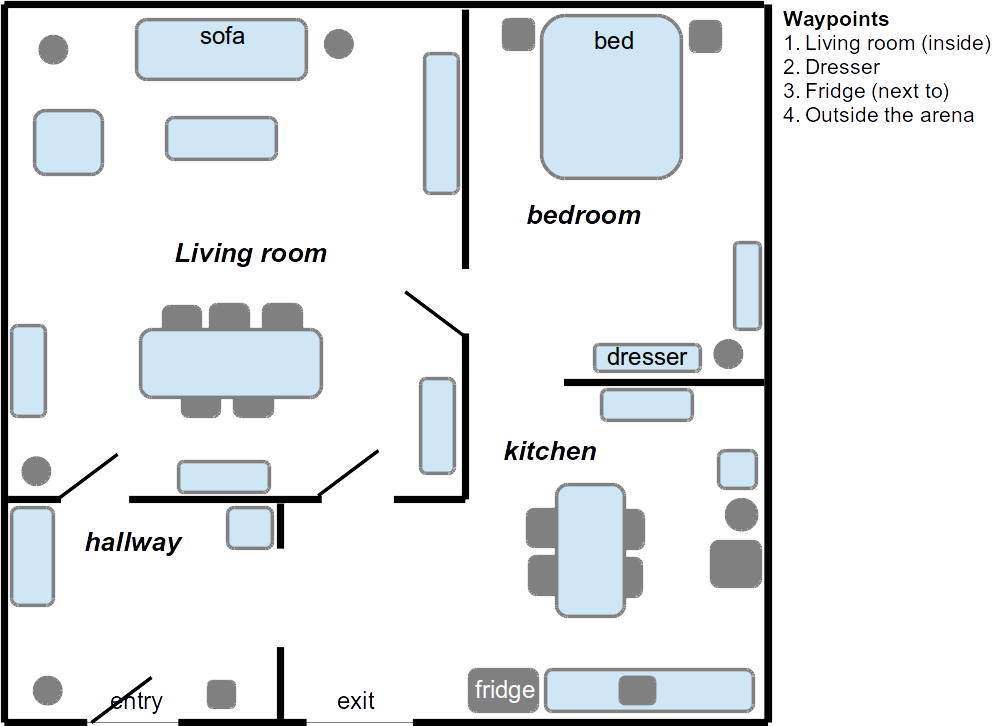
\includegraphics[width=0.5\columnwidth]{images/navigation.png}
	\caption{Navigation test: setup and execution example.}
	\label{fig:restaurant}
\end{figure}

\paragraph*{Remarks:}
\begin{enumerate}
	\item Depending on the layout of the arena, waypoint 1 and 2 may be swapped.
	\item Reaching a waypoint also includes the direction in which the robot should be looking when it reaches, which will be announced by the TC during the setup of the path.
	\item The distance between Waypoints 3 and 4 is about 10-20 meters.
\end{enumerate}

\subsection{Obstacles}
While navigating to waypoints 1, 2, and 3 the robot will find one of the following obstacles on its path:
\begin{itemize}
		\item \textbf{Small object:} Box sized object (between 5 and 15 cm per edge).  
		\item \textbf{3D Object:} A bar table, normal table, rolling chair: some object that is wider at its top than on its bottom, 
		  thus requiring more than just a laser scanner mounted near the ground to avoid obstacles.
		\item \textbf{Smart obstacle:} A person to whom the robot may speak to and kindly ask to move away. When interacting with people, the robot must look at the person and make clear is speaking with him/her.
	\end{itemize}

\subsection{Additional rules and remarks}
\begin{enumerate}
	\item \textbf{Waypoints:} Waypoints may be rooms, placement locations, furniture, beacons, landmarks, etc. The robot must clearly state when it has reached a waypoint or if it was not able to reach the waypoint.

	\item \textbf{Show must go on:} If a robot is unable to reach a waypoint, it must say it and proceed to the next one.

	\item \textbf{Closing internal doors:}  Theinternal door that will be shut will be the door on the route the robot has committed to. It will be shut right after the robot starts driving towards the door, but granting enough time to notice that the door is now closed.	

	\item \textbf{Moving objects:} If the robot finds on its way a \textit{static movable obstacle} (chair, cubes, toys, etc.) which is capable to move, it must announce is going to move an obstacle and then proceed to move the object apart with its manipulator, or by \textbf{gently} pushing it with its body.

	\item \textbf{Asking people to move away:} If the robot finds on its way a person blocking its path, it must announce it has found a person, \textit{gently} ask that person to move away and wait for the path to be clear. \textbf{Robots are not allowed to touch people}.

	\item \textbf{Following people:} 
	\begin{enumerate}
		\item \textbf{Instruction:} The robot interacts with the operator, \emph{not} the team. That is, the team is not allowed to instruct the operator.
		\item \textbf{Natural walking:} The operator has to walk \quotes{naturally}, i.e., move forward facing forward. 
		  The operator is not allowed to walk back, stand still, signal the robot or follow any re-calibration procedure.
		\item \textbf{Asking for passage:} The robot is allowed to (gently) ask people to step aside.
	\end{enumerate}
\end{enumerate}

\subsection{Data recording}
  Please record the following data (See \refsec{rule:datarecording}):
  \begin{itemize}
   \item Mapping data
   \item Plans
  \end{itemize}

\subsection{Referee instructions}

The referee needs to
\begin{itemize}
	\item Instruct the OC and volunteers on when and where locate objects.
	\item Instruct the OC and volunteers on when and which doors must be closed.
	\item Stop the robot immediately when it is about to collide.
\end{itemize}

\subsection{OC instructions}

\textbf{2 hours before the test}
\begin{itemize}
        \item Announce the entry and exit doors. 
	\item Announce the locations for waypoints 1, 2, and 3.
	\item Establish location for waypoint 4 and the path for the \textit{follow me} phase. 
\end{itemize}

\textbf{During the test}
\begin{itemize}
	\item Open and close the doors when instructed by the referee.
	\item Place the obstacles (or act as an obstacle) when instructed by the referee.
\end{itemize}

\newpage

\subsection{Score sheet}

The maximum time for this test is 5 minutes.

\begin{scorelist}

	\scoreheading{Waypoints}
	\scoreitem{10}{Reaching waypoint A}
	\scoreitem{10}{Reaching waypoint B}

	\scoreheading{Obstacles}
	\scoreitem{20}{Avoiding obstacle 1}
	\scoreitem{30}{Avoiding obstacle 2}
	\scoreitem{40}{Avoiding obstacle 3}
	\scoreitem{10}{Reporting unreachable waypoint due to an obstacle (will end the test)}

	\scoreheading{Doors}
	\scoreitem[2]{20}{Starting a new path after reaching a closed door}
	\scoreitem[2]{45}{Opening the door and continue instead of plan a new trajectory}

	\scoreheading{Optional tasks (up to 50 points)}
	\scoreitem{10}{Reaching waypoint}
	\scoreitem{40}{Reentering the arena after reach Waypoint 3}

	\setTotalScore{200}
\end{scorelist}


% Local Variables:
% TeX-master: "Rulebook"
% End:


% Local Variables:
% TeX-master: "Rulebook"
% End:


\newpage
% Speech and Person Recognition
\section{Speech and Person Recognition}
The robot has to identify unknown people and answer questions about them and the environment.

\subsection{Focus}
This test focuses on human detection, sound localization, speech recognition, and robot interaction with unknown people.

\subsection{Setup}
\begin{enumerate}
    \item \textbf{Location:} One room of the arena is used for this test.\footnote{This test may also be held outside the arena}.
    \item \textbf{Crowd:} There is a crowd of 5 to 10 people in the designated room. People may be standing, sitting, lying, and in any pose.
    \item \textbf{Doors:} All doors of the apartment are open, except for the entry door. 
\end{enumerate}

\subsection{Task}
\begin{itemize}
    \item \textbf{Start:} The robot starts at a designated starting position and announces it wants \textit{to play riddles}.

    \item \textbf{Waiting and turn:} After stating that it wants \textit{to play a riddle game}, the robot waits for 10 seconds while a crowd is merged on it's back. When the time elapses, the robot must turn around (about $180\degree$) and find the crowd.

    \item \textbf{Requesting an operator:} After turning around, the robot must state the size of the crowd (male and female count) and request for an operator (e.g.~\textit{who want to play riddles with me?}). The crowd will move and surround the robot, letting the operator to stand in front of the robot.

    \item \textbf{The riddle game:} Standing in front of the robot, the operator will ask 7 questions from the list.\\
    The robot must answer the question without asking confirmation. Questions will only be asked only once; no repetitions are allowed. 

    \item \textbf{The blind man's bluff game:} A random person from the crowd surrounding the robot will ask a question. The robot may
    \begin{itemize}
        \item Turn towards the person who asked the question and answer the question
        \item Directly answer the question without turning
        \item Turn towards the person and ask them to repeat the question
    \end{itemize}
    The game will end when the 7th question has been made, following the same distribution as in the riddle game. The robot must answer the question without asking confirmation. Questions may be repeated once.

    \item \textit{Leave:} The robot leaves the room through the designated door.
\end{itemize}

\subsection{Additional rules and remarks}

\begin{itemize}
    \item \textbf{Bypassing ASR:} Bypassing Automated Speech Recognition via the CONTINUE rule (Section \refsec{rule:asrcontinue}) is not allowed during this test.
    \item \textbf{Asked questions:} The distribution of questions to be randomly asked is a follows:
    \begin{itemize}
        \item One is a predefined question
        \item Two are about the arena and its status
        \item Between two and three are about the crowd
        \item Between two and three are about the list of official objects
    \end{itemize}
    Question examples see Appendix \refsec{chap:robogame-appendix}.
    \item \textbf{Distance to the robot:} The distance between each person and the robot must be between 0.75 and 1.0 meters away from the robot position (See Figure \ref{fig:asrsetup}). In the \textit{riddle game} the operator shall be between -60$^{\circ}$ and 60$^{\circ}$ from the robot's center (front range).
    \item \textbf{Precise turning:} When the robot finishes turning toward an operator, it must be clear that the robot is facing the person who made the question.
    \item \textbf{Question repetition:} In the \textit{blind man's bluff game}, if the robot asks for repetition, it should be done clear and loud, and after the robot has ended turning.
    \item \textbf{Question timeout:} If the robot does not answer within 10 seconds, the question is considered as \textit{missed}, and referee will proceed with the next one.
    \item \textbf{Standing still operators} Operators are not allowed to move to or turn towards the robot or shout to the robot.
    \item \textbf{Water-clear answers:} If the referee is unable to hear or understand the robot's answer, the question is considered as \textit{incorrect}. Single-word and short answers should be avoided
\end{itemize}

\begin{figure}[!h]
	\centering
	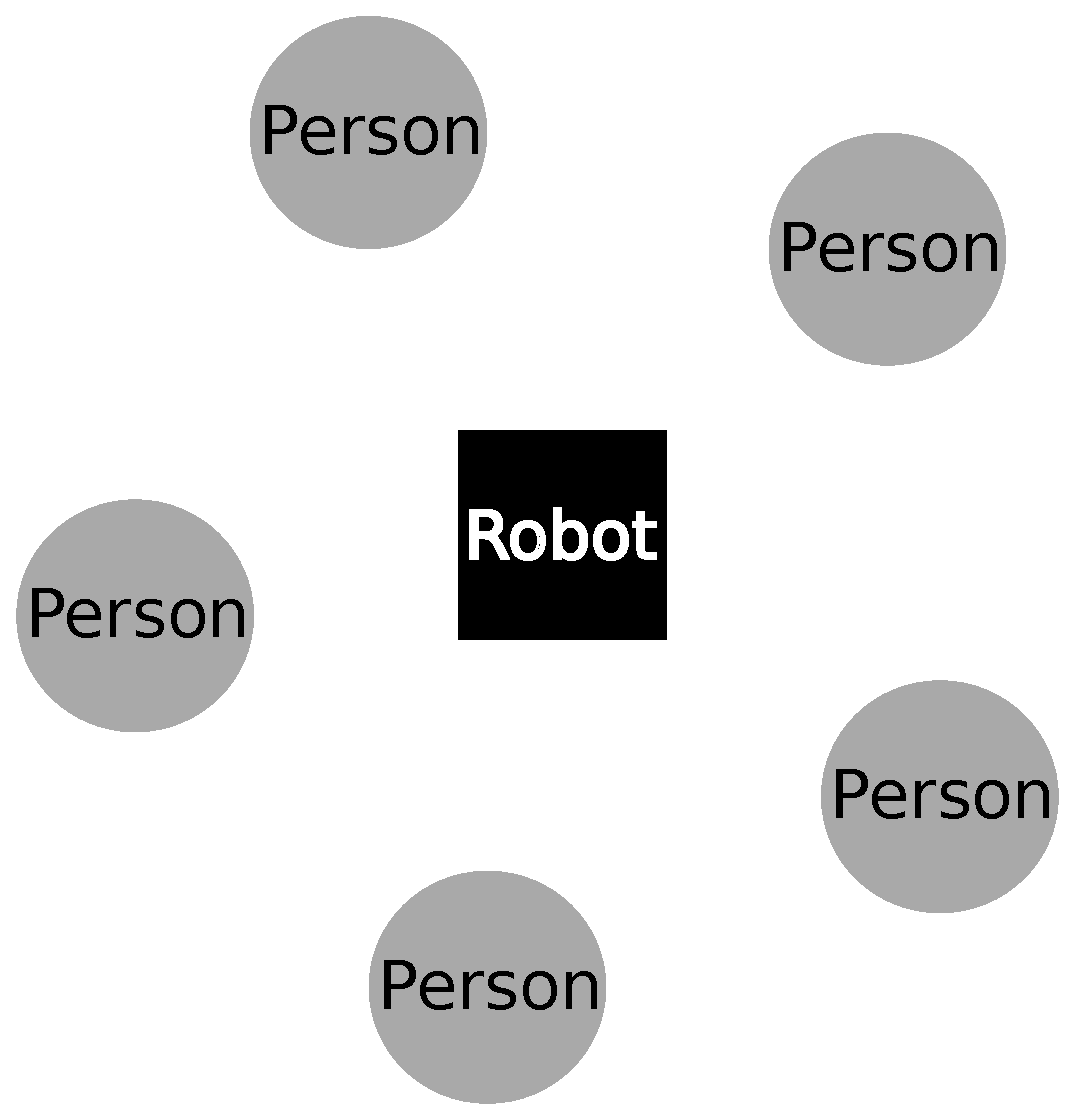
\includegraphics[width=0.5\columnwidth]{images/asrsetup.pdf}
	\caption{Speech recognition test: person setup around the robot for 2nd part.}
	\label{fig:asrsetup}
\end{figure}

\subsection{Data recording}
Please record the following data (See \refsec{rule:datarecording}):
\begin{itemize}
    \item Audio
    \item Commands
    \item Images
\end{itemize}

\subsection{Referee instructions}

The referee needs to
\begin{itemize}
    \item avoid shouting to the robot
    \item avoid getting closer to the robot (or even move)
    \item speak to the robot loud and clear with plain standard English
    \item avoid repeating questions for the same robot
    \item distribute the questions among the volunteers
\end{itemize}

\subsection{OC instructions}

\textbf{1 day before the test}
\begin{itemize}
    \item Provide the set of predefined questions
\end{itemize}

\textbf{2 hours before the test}
\begin{itemize}
    \item Announce the placement of the robots
    \item choose the volunteers for the second part of the test, and clearly explain the procedure to them.
\end{itemize}



\subsection{Score sheet}
The maximum time for this test is 10 minutes.

\begin{scorelist}

	\scoreheading{Crowd}
	\scoreitem{10}{State crowd's male/female count}

	\scoreheading{Riddle game}
	\scoreitem[8]{10}{Correctly answered a question}
	\scoreitem{5}{Answering all 8 riddle game question}

	\scoreheading{Blind man's bluff game}
	\scoreitem[8]{15}{Answering question on the first attempt}
	\scoreitem[8]{5}{Answering question on the second attempt}
	\scoreitem[8]{10}{Turned towards person asking the question}
	\scoreitem{5}{Answering all 8 blind man's bluff questions}

	\setTotalScore{300}
\end{scorelist}

% Local Variables:
% TeX-master: "Rulebook"
% End:


% Local Variables:
% TeX-master: "Rulebook"
% End:


\newpage
\section{Help-me-carry}
The robot's owner went shopping for groceries and needs help carrying the groceries from the car into the home.
The whole family helps, as well as the robot. 

\subsection{Goal}
The robot must bring some items from outside the arena inside the arena.

\subsection{Focus}
This test focuses on following and navigation in an unknown environment. 

\subsection{Setup}
The robot starts waiting inside the arena. 
The operator (the robot's owner) has a set of bags and boxes that need to be carried from a place outside the arena back inside. 

\begin{enumerate}
  \item \textbf{Location:} One of the arenas (apartment) and its surroundings. The apartment is in its normal state. Part of the test is performed outside the arena in a public space.
  \item \textbf{Start:} Starting location of the robot. %%Close *to* the front door of the appartment?
  \item \textbf{Car:} The robots operator has put the groceries in the trunk of the car after shopping. The operator parked the car outside the home.
  \item \textbf{Destinations:} The items must be transported to places where they can be stored. The destinations are various rooms of the arena. 
  \item \textbf{Doors:} All doors in the apartment are open.
  \item \textbf{Operator:} A \quotes{professional} operator is selected by the TC to act as the operator of the robot. 
  \item \textbf{Other people:} There are no restrictions on other people walking by or standing around throughout the complete task. 
\end{enumerate}

\subsection{Task}
\begin{enumerate}
\item \textbf{Start:} The robot is waiting somewhere in the apartment. The operator approaches the robot and tells it to follow.
\item \textbf{Following:} The robot starts following the operator, who guides the robot to the car containing the groceries. 
\item \textbf{Arrive at car:} When at the car, the operator tells the robot they have reached the car and to remember this location.
\item \textbf{Handover groceries:} The operator gives the robot a command to carry something, e.g. a box or a bag.  
  The robot puts up its arms and the operator gives the item to the robot.
\item \textbf{Command destination:} The operator of the robot tells where the given item should go, one of the rooms in the arena. 
\item \textbf{Delivery:} The robot then goes inside the house to deliver the item to the destination. 
\item \textbf{Repeat until time is up:} Then, the robot goes back to the car (by itself, as it already knows where the car is) to bring another item inside. 
\end{enumerate}

The robot may encounter some obstacles while navigating and the robot must deal and avoid or otherwise deal with the obstacle. 
The possible obstacles are:
\begin{itemize}
	\item \textbf{Small object:} Small object. For example, someone has dropped a piece of fruit (like an apple or mandarin) while carrying the groceries inside.
	\item \textbf{3D Object:} A bar table, normal table, rolling chair: some object that is wider at its top than on its bottom, 
	  thus requiring more than just a laser scanner mounted near the ground to avoid obstacles. 
	\item \textbf{Smart obstacle:} A person to whom the robot may speak to and kindly ask to move away. 
	  When interacting with people, the robot must look at the person and make clear is speaking with him/her.
	\item \textbf{Moving people:} As the whole family living in the house is helping getting the groceries from the car, 
	  additional to the robot there will be some people also going back and forth between the car and various rooms. 
	  The robot will encounter these and deal with them. These people are friendly to the robot and will not actively block it but the robot must also not block them. 
\end{itemize}
%% Possible extensions: 
%% - DONE: allow the operator to tell for each item where it should go
%% - At the destination room, there is a person waving, waiting for the robot to bring the items so (s)he can take them
%% - Points for a natural handover. E.g. the human is holding a box and the robot moves in to take it over instead of the humans placing it in the robots arms. Same for the bag
%% - Close the appartment door when the robot is inside?

\subsection{Additional rules and remarks}
\begin{enumerate}
  \item \textbf{Delivering items:} At the destination, the robot may place the bag or box at a convenient location: the floor or a table
  \item \textbf{Obstacle avoidance:} The robot will encounter some human(s) on the way between the two locations.  
\end{enumerate}

\subsection{Data recording}
  Please record the following data (See \refsec{rule:datarecording}):
  \begin{itemize}
   \item Maps
   \item Plans
  \end{itemize}

\subsection{Referee instructions}

The referee needs to
\begin{itemize}
\item Distribute some objects over some boxes and shopping bags.
\item Destignate a few ``car parking locations'' from which the objects must be carried.
\end{itemize}

\subsection{Score sheet}

The maximum time for this test is 4 minutes.

\begin{scorelist}
	\scoreheading{Single iteration}
	\scoreitem[3]{10}{Reach the car}
	\scoreitem[3]{1}{Accept the item from the owner}
	\scoreitem[3]{1}{Understand the commanded destination}
	\scoreitem[3]{6}{Reach inside the arena again}
	\scoreitem[3]{6}{Reach the destination}
	\scoreitem[3]{5}{Put the item at the floor or a nearby table}
	% 3x 30 points = 90 only
	
	% Up to 60 points
	\scoreheading{Obstacle avoidance}
	\scoreitem{5}{Avoiding box-sized object}
	\scoreitem{10}{Avoiding 3D object (Difficult-to-see object)}
	\scoreitem{5}{Asking a person to step aside}
	\scoreitem{30}{Moving away movable object}
	\scoreitem{10}{Move aside for person}
	
	\setTotalScore{150}
\end{scorelist}


% Local Variables:
% TeX-master: "Rulebook"
% End:


\newpage
\section{General Purpose Service Robot}

This test evaluates Human-Robot Interaction and the integration of the abilities of the robot tested in stage I. In this test the robot has to solve multiple tasks upon request. That is, the test is not incorporated into a (predefined) story and there is neither a predefined order of tasks nor a predefined set of actions. The actions that are to be carried out by the robot are randomly generated by the referees and are composed by 3 subtasks which include navigation, human-robot interaction and robot-object interaction.

The command is composed by three actions, which the robot has to show it has recognized. The robot may repeat the understood command and ask for confirmation. If it can't recognize the command correctly, it can also ask the speaker to repeat the complete command, or ask for further information.

\subsection{Focus}
This test particularly focuses on the following aspects:
\begin{itemize}
	\item No predefined order of actions to carry out (to get away from state machine-like behavior programming).
	\item Increased complexity in speech recognition (possible commands are less restricted in both actions/operators and arguments/objects, commands can include multiple objects, e.g., \quotes{put the apple on the kitchen table})
\end{itemize}

\subsection{Task}

\begin{enumerate}
	\item \textbf{Entering and command retrieval:} The robot enters the arena and drives to a designated position where it has to wait for further commands.
	\item \textbf{Command generation:} A command is generated randomly, depending on the command category chosen by the team (see below). \\

	\item \textbf{Command categories:} All possible actions has been classified previously by the TC according to their difficulty level. The team may choose from the following three categories:
	\begin{enumerate}
		\item \textbf{Category I:} Tasks with a low degree of difficulty (easy to solve). This category includes indoor navigation, grasping known objects, answering questions (from the predefined set of questions), etc.
		\item \textbf{Category II:} Tasks with a moderate degree of difficulty. This category includes following a human, indoor navigation in crowded environments, grasping alike objects, find a calling person (waving or shouting), etc.
		\item \textbf{Category III:} The same tasks as in category II. However, the information given to the robot will be incomplete or incorrect, meaning that the command as it is specified exactly is not possible. The robot must come up with an appropriate solution to meet the operators' command. Please see the Command examples below.
	\end{enumerate}

	\item \textbf{Task assignment:} The robot is given the command by the operator and may directly start to work on the task assignment. The robot must must prove it has understood the given command by repeating it (Please see the remarks about this in section~\ref{sec:gpsr_remarks}).
	\item \textbf{Exiting the arena:} After accomplishing the assigned task, the robot has to leave the arena.
\end{enumerate}

\subsection{Commands and actions}
The command is composed by three actions, which the robot has to show it has recognized. The robot may repeat the understood command and ask for confirmation. If it can't recognize the command correctly, it can also ask the speaker to repeat the complete command. If the robot fails to understand the given commands, it may ask to the operator to repeat them up to three times, if it fails the team may opt to use the Continue rule (Section \refsec{rule:asrcontinue}). In case the robot has understood partially the command, it may ask the operator for additional information (e.g.~\quotes{did you say apple juice or pineapple juice?}).

Required in this test are:
\begin{enumerate}
	\item abilities from stage I forming a set of actions $A$ (e.g., following a person, finding a random person, finding a person after memorizing her; finding, recognizing, grasping, and delivering objects, etc.),
	\item a set of people $P$,
	\item a set of questions $Q$,
	\item a set of objects $O$ (the same set as used as in the other tests),
	\item a set of locations $L$ (the same set as used as in the other tests).
\end{enumerate}

Each task assignment contains an action $a \in A$ and, depending on the respective action an object $o \in O$, a location $l \in L$, a question $q \in Q$, a person $p \in P$ to interact with, or a combination of those. The set of actions is not given beforehand, instead, teams should identify the abilities from Stage I by themselves (and find synonyms for that). That is, $L$, $O$ and $Q$ are known in advance (provided during setup days), but $A$ has to be \quotes{found out} by the teams (e.g.~taken from freely available ontologies, synonym searches etc.). For the actions $A$ are going to be used common synonyms (like \quotes{go to}, \quotes{move to}, \quotes{drive to}, and \quotes{navigate to} to describe navigation). For the people $P$, any person willing to operate the robot in a natural way can be expected, however, \quotes{Professional Operators} are more likely to be used.

\paragraph{Command examples}
\begin{enumerate}
	\item \textbf{Category I}
	\begin{itemize}
		\item Go to the bedroom, find a person and tell the time (there is only one person in the bedroom).
		\item Go to the dinner-table, grasp the crackers, and take them to the side-table.
		\item Bring a coke to the person in the living room and answer him a question (there is only one person in the bedroom).
		\item Go to the door, ask the person there for her name and tell it to me.
	\end{itemize}
	\item \textbf{Category II}
	\begin{itemize}
		\item Go to the bedroom, find the waving person and tell the time (there is more than two people in the bedroom, only one waving).
		\item Go to the kitchen, find a person and follow her (there is only one person in the kitchen).
		\item Go to the side-table, grasp the coke, and take it to the dinner table (the way to the bedroom is crowdy and the access to the side-table may be blocked by a human).
		\item Go to the dinner-table, grasp the banana, and take it to the side-table.
	\end{itemize}
	\item \textbf{Category III}
	\begin{itemize}
		\item Take the apple from the sink and carry it to me. 
		  (There may no apple in the sink, but maybe another fruit the operator might want, an apple my be found somewhere else, etc.)
		\item Go to the kitchen, grasp the coke, and take it to the side-table.
		  (There may no coke in the kitchen but some other drink.)		
		  \item Go to the bathroom, grasp the soap, and take it to the side-table.
		  (The door to the bathroom may be closed. The robot must open the door, find a soap somewhere else or ask someone to open the door for it.)
		\item Grasp the fanta from the small table and carry it to me.
		  (When the robot comes back with the drink, I have moved somewhere else and the robot must find me again.)
	\end{itemize} 
\end{enumerate}

\subsection{Additional rules and remarks}
\label{sec:gpsr_remarks}
\begin{enumerate}
	\item \textbf{Referees:} Since the score system in this test involves a subjective evaluation of the robot's behavior, the referees are EC/TC members.
	\item \textbf{Operator:}
	\begin{itemize}
		\item The person operating the robot is one of the referees (default operator).
		\item If the robot appears to consistently not be able to understand the operator, the referees ask the team to continue with a custom operator (Section \refsec{rule:operator}).
		\item With the custom operator, the team can only score 50\% of the points for the respective command.
	\end{itemize}
	\item \textbf{Repeating the given command:} The robot must show it has understood the given command by stating all the required information to accomplish the task. This doesn't mean the robot must repeat exactly the same given command. For instance, if the robot is instructed to \textit{\quotes{deliver a coke to Mary in the kitchen}}, the robot may ask: \textit{\quotes{do you want me to go to the kitchen, find Mary and deliver a coke to her?}} or \textit{\quotes{do you want me to find Mary at the kitchen and give her a coke?}} since both sentences involve all given information.
	\item \textbf{Asking reasonable questions} 
	\begin{enumerate}
		\item \textbf{Misunderstood information:} When the robot did not understood part of a command or it is unsure of what has been told, it may ask the operator to repeat or clarify without fall into a new attempt. For instance, if the robot is instructed to \textit{\quotes{bring me the apple juice from the kitchen table}}, a valid question for the robot to ask is \textit{\quotes{did you say apple juice or pineapple juice?}} without considering it as a new attempt for giving the command.
		\item \textbf{Missing information:} When a given command lacks of information required for accomplishing the task, the robot should request for that missing part. For instance, if the robot is instructed to \textit{\quotes{offer a drink to the person at the door}}, a proper question for the robot to ask is \textit{\quotes{which drink should I deliver to the person at the door?}} It is also possible that the robot simply confirms the command and fetch a random drink at drinks' location, however, no points will be scored for solving that part.
		% \item \textbf{Nonsenseness:}
	\end{enumerate}
	\item \textbf{Following people} 
	\begin{enumerate}
		\item \textbf{Instruction:} The robot interacts with the operator, \emph{not} the team. That is, the team is not allowed to briefly instruct the operator.
		\item \textbf{Natural walking:} The operator has to walk \quotes{naturally}, i.e., move forward facing forward. The operator is not allowed to walk back, stand still, signal the robot or follow some re-calibration procedure.
		\item \textbf{Asking for passage:} The robot is allowed to (gently) ask people to step aside.
		\item \textbf{Stopping:} The robot must decide when to stop following a person, either because it was instructed to follow her to a certain location, because it was asked to stop by the operator or because the test time is running out. In any case, the robot should state the reason why it changes its behavior.
	\end{enumerate}
\end{enumerate}

\subsection{Referee and OC instructions}
\textbf{2h before test:}
\begin{itemize}
\item Specify and announce the entrance and exit door
\end{itemize}
\textbf{During the test:}
\begin{itemize}
\item Generate random sentences by an automatic sentence generator
\end{itemize}

\newpage
\subsection{Score sheet}
The maximum time for this test is 6 minutes.
\begin{scorelist}
	\scoreheading{Getting instructions}
	\scoreitem{40}{Understanding the set of actions on the $1^{st}$ attempt}
	\scoreitem{20}{Understanding the set of actions on the $2^{nd}$ attempt}
	\scoreitem{10}{Understanding the set of actions on the $3^{rd}$ attempt}
	\scoreitem[0.5]{-1}{Reduction of points for every command provided by a team member}

	\scoreheading{Performing the task: Category I}
	\scoreitem{10}{Performing the first task correctly}
	\scoreitem{10}{Performing the second task correctly}
	\scoreitem{30}{Successfully solving the complete command}

	\scoreheading{Performing the task: Category II}
	\scoreitem{20}{Performing the first task correctly}
	\scoreitem{30}{Performing the second task correctly}
	\scoreitem{50}{Successfully solving the complete command}

	\scoreheading{Performing the task: Category III}
	\scoreitem{10}{Asking reasonable questions to obtain missing information}
	\scoreitem{30}{Performing the first task correctly}
	\scoreitem{60}{Performing the second task correctly}
	\scoreitem{80}{Successfully solving the complete command}
	\scoreitem{30}{Explaining how the original command was not possible in it's (incorrect) statement and how this was solved}

	\setTotalScore{250}
\end{scorelist}

% Local Variables:
% TeX-master: "Rulebook"
% End:


% Local Variables:
% TeX-master: "Rulebook"
% End:


\chapter{Tests in Stage II}
\label{chap:stage_II}

\begin{itshape}
All ability and integration tests in \iterm{Stage~II} grants 250 points (but the \iterm{Open Challenge} which grants 250) and are performed only once. Some tests have optional tasks that grant additional points when performed correctly, clean and fast. The \iaterm{Technical Committee}{TC} must be informed if a team is planning to perform any of the optional tasks. Unless explicitly stated otherwise, no additional time is given while performing optional tasks.

In the \iterm{Open Challenge} the robot must be able to show to the \iaterm{Technical Committee}{TC} the achievements on the main research line of its own team. This test grants up to 200 points.

\section{Robot \& team cooperation}
We encourage robots and teams to work together when performing challenges.
For scoring, points are awarded per subtask. The robot (and thus team) performing the subtask gets the points.
For example, in the Restaurant-challenge, if one robot of team A can take the order and another robot of team B delivers the order, then the points for taking the order go to team A, while the points for delivering go to team B. 
Of course, team A \& B can both perform the challenge in their own turn.

\end{itshape}

\newpage
\section{Set a table and clean it up}

Setting up a table for a meal and cleaning it up afterwards is one of the most repetitive tasks in a household environment. How wonderful it would be to have a robot doing it for us? This tasks aims at evaluating the capability of robots at this task.

The task comprises two phases: in phase~I, the robot is asked to set up the table, according to an optional variation given by the referee, and in the phase~II, the robot is supposed to cleanup the table, returning all placed objects to their original location, including detecting and cleaning spills with a cleaning cloth.

This task takes place in a single room, designated \emph{kitchen,} with a \emph{table,} where the relevant objects are stored, some of then on an open closet and other on a closed closet.

In phase~I, the operator requests the robot to setup the table for a meal. In this request, the operator may specify one variation of the meal, e.g., milk or coffee, bread or cookies. The robot should then set the table using items stored in various places of the kitchen, and afterwards it must clean it up, including small spills on the table. Some of the items are easly accessible (e.g., over the kitchen counter) while others may require the opening of doors (e.g., inside a cloret). Furthermore, some of these items may constrain the way they are handled by the robot (e.g., avoid pouring contents of a container). These items must be placed on a table reasonably following social conventions in terms of their positions on the table\footnote{Strict adherence to any social convention is out of the scope of the competition, and thus will not be evaluated.}. Midway during placement, the robot owner may change/adjust the position of some of the items; the robot is expected to handle the situation appropriately.

In phase~II, the operator requests the robot to clean up the table. This includes both returning the placed objects to their original location, and cleaning up dirt and spills using a cleaning cloth. This requires the robot to memorize the location the objects were originally recognized.


\subsection{Example}

The operator requests the robot to set the table for breakfast. Then, the robot replies asking whether the operator prefers bread or cookies, to which the operator replies prefering bread.  Several items are placed on the table: a plate, cutlery, a cup, napkins, a basket with bread, a cereal box, etc. The basket with bread, a napkin, and the cereal box are on the kitchen counter; the plate, the cutlery, and the cup are inside a closet. The robot starts moving these items, one by one, from their original position to the table. Some of these objects pose specific challenges to robot manipulation: the napkin is a flexible object, the bread basket contains bread, thus the robot must hold it with care, the items inside the closet require the closet door to be opened, and the cutlery is non-trivial to grasp. After the bread basket is placed on the table, the robot owner decides to move its place, so the positioning of remaining objects must have this in consideration. Then the robot will await an instruction by the operator to clean up the table. While taking his/her meal, the table gets dirty with a spill. The robot must detect the spill and clean it up using a cleaning cloth. Then, all of the other items are returned to their original locations. The task concludes once the table returns to its original state.

\subsection{Goal}

The robot has to move a list of relevant objects, with a possible variation stated by the operator, onto the a predefined table in the kitchen. Then it should return all placed items to their original locations and cleanup dirt ansd spills from the table.

\subsection{Focus}

This test focuses on HRI, semantic mapping, object perception and manipulation.

\subsection{Setup}

Half of the objects are placed on the kitchen counter, while the remaining ones inside a predefined closet, which is closed before the robot entering the arena. The table should be initially cleared of any objects. The robot will start at a predefined location, away from both the kitchen counter and the table. The team may optionally specify to the referees the variations supported by the robot, with at least two options. The referee then selects one of them randomly, not disclosing the choice.

\subsection{Task}
\label{sattu:task}

\begin{enumerate}
\item \textbf{Requesting the task:} The operator requests the robot to set up the table.
\item\label{sattu:s2} \textbf{Asking for variation:} (optional) The robot asks the operator for an option, to which the operator replies with the randomly selected (and undisclosed) option.
\item \textbf{Searching for objects:} The robot must detect which objects are missing on the table and search for them either on the kitchen counter on inside the closet.
\item \textbf{Grasping objects:} The robot must grasp any missing object and move it to the table.
\item \textbf{Placing objects:} Each object must be placed in a socially accepted position, not coliding with any object there.
\item \textbf{Changing objects position:} The operator will change the position of two objects on the table at any time, before the placement of the last one.
\item \textbf{Cleaning up the table:} After the meal, the operator requests the robot to clean up the table. The robot returns the objects to their original location, \textit{i.e.,} where they were found in the first place.
\item \textbf{Cleanup dirt and spills:} The robot must detect dirt and spills on the table and clean them up using a cleaning cloth.
\end{enumerate}

\subsection{Additional rules and remarks}
\label{sattu:add}
\begin{enumerate}
\item \textbf{No setup:} The robot must be ready to start the test with a voice command or start button when requested by the referee. There is no setup time.
\item \textbf{Startup:} The robot must be started with a single voice command or via a start button (Section \refsec{rule:start_signal}). If the robot is unable to start it must be removed immediately.
\item \textbf{Single try:} The robot must be able to start from the first attempt. 
`There is no restart for this test. If the robot is unable to start it must be removed immediately.
\item \textbf{Collisions:} Slightly touching the table.
  Driving over the objects or any other form of a major collision is not allowed, and the referees directly stop the robot (Section \refsec{rule:safetyfirst}).
\item\label{sattu:objs} \textbf{Object types:} The objects selected from the \textit{Standard Objects Set} will be chosen to be easily detectable and contrasting with the background (kitchen counter or closet). A maximum of 6 objects is considered for this task, where two of them is hard to grasp, e.g., cutlery, and another two must be handled upright, e.g., cup.
\item \textbf{Recognition report:} Robots must create a PDF report file including the list of recognized objects with a picture showing the object and the object name/label.
  This file may be stored on a USB-stick on the robot which is given to the TC after the test. The PDF file name should include the team name and a timestamp. 
  Furthermore, it must be unmistakeable which label belongs to which object. Objects must also be recognizable in the report by a human (TC) so that it can be scored. 
%  An overview of the shelf with bounding boxes and labels attached to the bounding boxes is handy for the TC to score.
False positives in the report (labeling an object which is not an object but e.g. the edge of the shelf) are penalized.
%\item \textbf{QR Codes:} The team may request to use a special set ob objects identified with QR codes if the robot is not able to correctly recognize the objects. The use of this special QR-object-set must be announced to the TC at least on hour before the test starts. When QR Codes are used, no points are given for object recognition.
\item \textbf{Clear area:} The robot may assume that there are no obstacles between the table, the kitchen counter, and the closet.
\item \textbf{Object list:} A total of 6 objects is considered, 3 of them considered easy to grasp (e.g., a cereal box, a cup, and a plate), while the remaining 3 hard to grasp (e.g., cutlery, napkins, and a basket with bread).
\item \textbf{Task variation:} The team may provide the referees a written set of options for setting up the table. These options must be written as possible answers to the robot question (step~\ref{sattu:s2} in section~\ref{sattu:task}). The correct execution of the specified variation should be clearly visible, e.g., choice of an object placed on the table.
\end{enumerate}

\subsection{Data recording}
  Please record the following data (See \refsec{rule:datarecording}):
  \begin{itemize}
   \item Images of recognized objects
   \item List of moved items
  \end{itemize}

\subsection{Referee instructions}

The referee needs to
\begin{itemize}
\item Clean up any remaining object on the table.
\item Place the objects on either the kitchen counter or inside the closet, half of them in each one of these two locations. Each one of these locations must contain at least one easy to grasp and one hard to grasp object.
\item Close the closet door.
\item Ask the team whether they implemented a meal variation, and if yes, choose randomly one of the options, not disclosing the choice.
\end{itemize}

\subsection{OC instructions}

The Organization must provide:
\begin{itemize}
\item the objects, as specified in item~\ref{sattu:objs} of section~\ref{sattu:add}
\item both an open closet and a closet with a door in the kitchen room
\end{itemize}


\subsection{Score sheet}

The maximum time for this test is \textbf{10 minutes}. A maximum of 6 objects is
considered in this score sheet. 3 of those are easy to grasp, 3 are difficult to grasp (for a robot)

\begin{scorelist}

  \scoreheading{Meal variation}
  \scoreitem[1]{10}{For asking for the meal variation and confirming the choice}

	\scoreheading{Grasping objects}
	\scoreitem[12]{10}{For each successful grasp of any object (lifting it up to at least 5 cm for more than 10 seconds)}
	\scoreitem[12]{15}{For each successful grasp of an hard to grasp object (lifting it up to at least 5 cm for more than 10 seconds)}
        % Grasping = (* 12 (+ 10 15)) = 300

	\scoreheading{Placing objects}
	\scoreitem[6]{10}{For each successful placement of any object anywhere on the table (safely stands still for more than 10 seconds)}
	\scoreitem[6]{20}{For each successful placement of an hard to grasp object anywhere on the table (safely stands still for more than 10 seconds)}
        \scoreitem[1]{30}{For appropriately executing the operator's choice}
	\scoreitem[6]{-5}{For each collision of an object with another
        one on the table}
        % Placing = (+ (* 6 (+ 10 20)) 30) = 210

      \scoreheading{Cleaning up the  table}
	\scoreitem[6]{10}{For each successful placement of any object to its original location}
	\scoreitem[6]{20}{For each successful placement of an hard to grasp object to its original location(safely stands still for more than 10 seconds)}
        \scoreitem[1]{40}{For successfully cleaning up dirt and spill on the table}
        % Cleaning = (+ (* 6 (+ 10 20)) 40) = 220
	
% 	\scoreheading{Total task}
% 	\scoreitem[5]{40}{Place known object near known object of same class}
% 	\scoreitem[5]{50}{Place unknown object near unknown object of same class}

        \scoreheading{Bonus}
        \scoreitem[1]{15}{Open the door without human help}

	% (+ 10 Grasping Placing Cleaning Bonus))
	\setTotalScore{745}
\end{scorelist}

% \subsection{Score examples} 

% TODO

% \begin{itemize}
%  \item Robot A fails at all manipulation attemps but makes an excelent report, with the 5 known objects labeled correctly and the 5 pairs of unknown objects correctly, will get 
% $5*10 + 5*15 = 125$ points. 
%  \item Robot B that fails to recognize anything but does move all the objects from the table to anywhere in the cupboard receives $5*10 + 5*10 = 100$ points.
%  \item Robot C grasps a single unknown item (``Cookies''), places it at the correct position near the other ``Cookies'' and also makes the same excelent report as robot A will get 
% 10 points for grasping, 10 foor placing anywhere and an additional 5 for placing at the right location, so 25 for that single object.
% The  total for robot C is then 150 points.
% \end{itemize} 


% Local Variables:
% TeX-master: "Rulebook"
% End:


% Local Variables:
% TeX-master: "Rulebook"
% End:


\newpage
\section{Tour guide [SSPL only]}
The robot guides spectators to the audience area and answer their questions after explaining what's @Home about.

\subsection{Focus}
This test focuses in safe outdoor navigation, people detection, gesture recognition, unconstrained natural language processing, and Human-Robot Interaction

\subsection{Setup}
\begin{itemize}
	\item \textbf{Location:} This test takes place outside the arena in a public space close to the @Home area.

	\item \textbf{Other people:} There are no restrictions on other people walking by or standing around throughout the complete task.

	\item \textbf{In Parallel:} This test can run in parallel, with several teams tested simultaneously.
\end{itemize}

\subsection{Task}

\begin{enumerate}
	\item \textbf{Start:} The robot waits at a designated starting position for the referee to give the start signal. When the referees start the time, the team is allowed to (briefly) provide some remarks about the robot's operation. After the instruction, the referee gives the start signal to the robot.\\

	\item \textbf{Finding spectators:} The robot starts moving to an open area and looks for (preferably large) groups of people. Once located the robot must approach to the spectators while calling for their attention in a \emph{friendly} way.\\

	People trying to call the attention of the robot (e.g. by waving or shouting) have priority over those just walking by despite the number of the crowd. The robot may also approach to a single person.\\

	\item \textbf{Greeting an spectator:} Once the robot has gained the attention of the spectators, it must introduce itself (i.e. saying it's name), and greet one of the spectators as customary in the venue's country (e.g. bowing, handshaking, waving, etc).\\

	Note that all spectators may also want to greet the robot. The robot is expected to be polite and continue greeting on demand.\\

	\item \textbf{Guiding the spectators:} The robot must gently ask the spectators to follow it to any of the @Home audience areas and guide them there. Should the people not be willing to follow the robot, it must thank them and start looking for another group of spectators.\\

	\item \textbf{Explaining the league:} Once at the @Home audience area, the robot must ask the spectators to take seat. The robot proceeds to \textit{briefly} introduce RoboCup@Home and explain the Social Standard Platform League's objectives. \\

	\item \textbf{Answering questions:} At the end of the speech, the robot asks for questions from the spectators regarding what it just explained, answering at least two of them. The robot is allowed to rephrase questions before answering them.\\

\end{enumerate}

\subsection{Additional rules and remarks}
\begin{enumerate}
	\item \textbf{Safety First!} The robot will be stop at the slightest possibility of a human being harmed or molested. The robot must not force interaction with humans, nor scare them or make them feel uncomfortable. \\

	\item \textbf{Referee guard:} During the entire test, a referee will be following the robot from behind for keeping people safe and for scoring purposes.\\
	
	\item \textbf{Approaching to spectators:} When approaching to people the robot should act in a natural way by reducing its velocity as it approaches to the people. The robot must look safe and friendly.\\

	Shall the people flee, the robot must not chase them.\\

	\item \textbf{Spectators:} Spectators are people attending to the venue to see the competition with no restriction of any kind, therefore, their numbers, grouping, and behaviour are not controlled by the league. Were the case of no spectators available, volunteers can be used instead.\\

	\item \textbf{Bilingual robots:} Robots are allowed (and encouraged) to interact with people in a language other than English. In such cases, the robot must utter the English equivalent right after synthesising the localized sentence. \\

	Notice that spectators may prefer to ask questions in their native language when interacting with a bilingual robot. In such cases, the robot must translate the question for the Referee to understand it and answer the question in both languages.\\

	\item \textbf{Handshaking:} When handshaking, the robot must stay at a safe distance from the people (e.g. about 1.5m) and reach out its \textit{hand}, but it must be a human, not the robot, who accepts and completes the handshake. If the human refuses to shake hands, the robot must retreat its manipulator immediately.\\

	\item \textbf{Disturbances from outside:} If a person from the audience (severely) interferes with the robot in a way that makes it impossible to solve the task, the team may repeat the test immediately.\\

	\item \textbf{Show must go on:} If the robot has engaged with a group of spectators when the allotted time for the test elapses, the robot is allowed to continue and finish the demonstration. However, no points are scored once the test is over.
\end{enumerate}

\subsection{Referee instructions}

The referees need to
\begin{itemize}
	\item Follow the robot at any time.
	\item Immediately stops the robot when considered necessary.
	\item Verify that the given answers are correct.
\end{itemize}

\subsection{OC instructions}

2h before test:
\begin{itemize}
	\item Recruit volunteers for the test (just in case).
	\item Announce the Start Location for the robots.
\end{itemize}

During the test:
\begin{itemize}
	\item Keep at least one area free in the audience area for robots to perform there.
	\item Send volunteers to join the Q\&A session to ask questions if necessary.
\end{itemize}

\newpage 
\subsection{Score sheet}
The maximum time for this test is \textbf{10 minutes}.

\begin{scorelist}
	\scoreheading{Engaging spectators} % Max 50
	\scoreitem{30}{Find an spectator (or group)}
	\scoreitem{20}{Greet an spectator (handshake)}
	\scoreitem{10}{Greet and get greet by an spectator (bowing or waving)}

	\scoreheading{Guiding spectators} % Max 50
	\scoreitem{10}{Convince spectator to follow}
	\scoreitem{40}{Reach the audience area}

	\scoreheading{Q\&A Session} % Max 210
	% \scoreitem{10}{Finish talk without loosing spectators attention}
	\scoreitem{10}{Finish talk without loosing spectators}
	\scoreitem[2]{70}{Each correctly understood question}
	\scoreitem[2]{30}{Each correctly answered question}
	
	\scoreheading{Bilingual interaction} % Max 80
	\scoreitem{10}{Bilingual engaging}
	\scoreitem[2]{25}{Questions in $3^{rd}$ language}
	\scoreitem[2]{10}{Question answered also in $3^{rd}$ language}
	
	\setTotalScore{390}
\end{scorelist}


% Local Variables:
% TeX-master: "Rulebook"
% End:


\newpage
\newcommand{\bonusRobotCoop}{50~}

\section{Open Challenge}
\label{sec:test_open_challenge}

During the Open Challenge teams are encouraged to demonstrate recent research results and the best of the robots' abilities. It focuses on the demonstration of new approaches/applications, human-robot interaction and scientific value.

\subsection{Task}

The Open Challenge consists of a demonstration and an interview part. 
It is an open demonstration which means that the teams may demonstrate anything they like.  
The performance of the teams is evaluated by a jury consisting of all team leaders, TC and EC.
\OpenDemonstrationTask{seven}{three}

\subsection{Presentation} 
During the demonstration, the team can present the addressed problem and the demonstrated approach.
\begin{itemize}
\item A video projector or screen, if available, may be used to present a brief (max. 1 minute) introduction to what will be shown. 
\item The team can also visualize robot's internals, e.g., percepts. 
\end{itemize}

It is important to note that the jury may decide to end the demonstration if there is nothing happening or nothing \emph{new} is happening.

\OpenDemonstrationChanges

\subsection{Jury evaluation}
\begin{enumerate}
  \item \textbf{Jury of team leaders:} All teams have to provide \emph{one} person 
  (preferably the team-leader) to follow and evaluate the entire Open Challenge.
  \item \textbf{Evaluation:} Both the demonstration of the robot(s), and the answers of the team in the interview part are evaluated.\\ 
  For each of the following \emph{evaluation criteria}, a maximum of \scoring{10 points} is given per jury member:
  \begin{enumerate}
  \item Overall demonstration
  \item Human-robot interaction in the demonstration
  \item Robot autonomy in the demonstration
  \item Realism and \emph{usefulness for daily life} (Can this robot become a product?)
  \item Novelty and (scientific) contribution (+contribution to the community)
  \item Difficulty and success of the demonstration 
  \end{enumerate}
  A jury member is not allowed to evaluate and give points for the own team.
  \item \textbf{Normalization and outliers}: 
  \begin{enumerate}
    \item The points given by each jury member are scaled to obtain a maximum of \scoring{250 points} (i.e., multiplied by $\nicefrac{25}{6}$). 
    \item The total score for each team is the mean of the jury member scores.
      To neglect outliers, the $N$ best and worst scores are left out:
      $$\mbox{score} = \frac{\sum\mbox{team-leader-score}}{\mbox{number-of-teams} - (2N+1)},
      \quad N=\begin{cases}2, & \mbox{number-of-teams} \ge 10\\1, & \mbox{number-of-teams} < 10 \end{cases}$$
    \end{enumerate}
\end{enumerate}

\subsection{Additional rules and remarks}
\begin{enumerate}
	\item \textbf{Start signal:} There is no standard start-signal for this test.
	\item \textbf{Abort on request:} At any time during the demonstration, the jury may interrupt and abort the demonstration:
	\begin{enumerate}
		\item if nothing is shown: in case of longer delays (more than one minute), e.g., when the robot does not start or when it got stuck;
		\item if nothing new is shown: the demonstrated abilities were already shown in previous tests (to avoid dull demonstrations and push teams to present novel ideas).
	\end{enumerate}

	\item \textbf{Team-team-interaction:}  An extra bonus of up to \bonusRobotCoop points can be earned if robots from two teams (4 robots maximum, 2 from each team) successfully collaborate (robot-robot interaction).
	\begin{enumerate}
		\item This bonus is earned for both teams.
		\item The robot(s) of the other team must only play a minor role in the total demonstration.
		\item It must be made clear that the demonstrations from the two teams are not similar, otherwise the points cannot be awarded.
		\item In case a team receives two (or more) bonuses, the maximum bonus will be taken.
		\item The collaboration is possible even if one of the two teams has not reached Stage 2.
		\item The team which does not participate in Stage 2 receives no points for this test.
	\end{enumerate}
\end{enumerate}


% Local Variables:
% TeX-master: "Rulebook"
% End:


\newpage
\section{Restaurant}
The robot is tested in a real environment such as a real restaurant or a shopping mall.

\subsection{Focus}
This test focuses on online mapping, safe navigation in previously unknown environments, gesture detection, human-robot interaction, and manipulation in a real environment.

The robot will need to create its own map from the environment and then move into it to handle human requests, such as delivering drinks or snacks, while people are walking around.

\subsection{Setup}
\begin{enumerate}
	\item \textbf{Location:} A real restaurant fully equipped with a \quotes{Professional Waiter} and at least three tables with \quotes{Professional Clients}. 
\end{enumerate}

\subsection{Task}
\begin{enumerate}
	\item \textbf{Instruction:} In case the robot can work with a \quotes{Professional Waiter}, the team should very briefly instruct the waiter how to command the robot, e.g. what to say when a table location must be memorized etc.
	
	\item \textbf{Start:} The robot starts at a designated starting position, and waits for the \quotes{Professional} operator. When the referees start the time, the team is allowed to (briefly) instruct the operator. After the instruction, the operator steps in front of the robot and tells it to follow (no start signal).

	\item \textbf{Memorizing the operator:} The robot has to memorize the operator. During this phase, the robot may instruct the operator to follow a certain setup procedure.

	\item \textbf{Guide phase:} Starting from the \textit{Kitchen}, the robot is guided through the environment by a \quotes{Professional Waiter} which shows to the robot the location of each of the tables, its number, and on which side the table is (there is a total of 3 tables). After visiting all the tables, the robot must be guided again to the \textit{Kitchen}, to the same place where the guide phase started.

	\begin{itemize}
		\item \textbf{Own \textit{Professional Waiter} [Optional]:} Team Leader may choose to use their own custom \textit{Professional Waiter} for this test instead of the one provided by the committee. The Team Leader must inform a TC member at least one hour before the competition. When using a custom \textit{Professional Waiter}, no points are earned for state the side of the table.
		\item \textbf{Finding the tables [Optional]:} Team Leader may choose not to tell the robot on which side (left or right) is the table, and let the robot find the tables by itself. When using this option, the robot must state where the table is (i.e.~by telling: \textit{the table is to my right}).
	\end{itemize}

	\item \textbf{Ordering phase:}
	\begin{enumerate}
		\item \textbf{Which table to attend:} Once back in the kitchen, the robot shall ask to the \textit{Professional Waiter} to which table go first to take an order from. 
		  The robot has to go to the indicated table and ask for an order there.
		  This interaction of telling the robot which table to attend should be natural. 
		  Just saying ``1'' to the robot is not natural, you would not say this to a person either who has to attend table 1.
		  
		\item \textbf{First order (Table A)}: The robot must aks the person what he or she wants to order. See Orders below for details about ordering.

		\item \textbf{Detecting a call (Table B or C):} At any time while attending Table A's guests (going to fetch an order, asking the client, or returning to the kitchen with the order), a guest at Table B or C will ask for the robot's attention by waving \emph{and} calling it out using voice. 
		  The robot must state out loud that it has detected the call and that it will attend as soon as possible.
		  If the robot does not detect such a call, it may be given a command to go to the next table when it is back at the kitchen after finishing table A's order.

		\item \textbf{Second order (Table B or C):} After taking the Table A client's order, and if the request was detected, the robot must go to the table of the waving/calling person and ask for an order.
		  

		\item \textbf{Avoiding random citizen:} At any time while going to any of the tables or to the \textit{Kitchen}, a person may step on the robot's path. It is expected the robot to avoid that person or stop and wait for it to move away.
	\end{enumerate}

	\textbf{Orders:} The menu offers Beverages and Combos. An order may be a Beverage or Combo. One guest will order a Combo while the other will order a Beverage.
	  A Combo is a combination of two of the food items from the set of objects \ref{rule:scenario_objects}, e.g. ``noodles with peanuts'' or ``noodles and peanuts''. 
	  Guests also prefere to state their order in a natural way, as their would in a restaurant operated by humans. 

	\textbf{Note:} Table A, B and C may be any of Table 1, 2, 3, \dots, N in any order.

	\item \textbf{Delivering phase:}
	\begin{enumerate}
		\item \textbf{Repeating the order:} Once again in the kitchen, the robot recites the orders for each table, including the table number (e.g.~\textit{Hamburger with fries for table 1 and Orange juice for table 2}), to the \textit{Professional Barman}. This includes determining the table number of the waving/calling person. The \textit{Professional Barman} will serve the order and place it into a tray on the Kitchen-bar.
		  If the barman cannot understand the order that the robot repeats, he cannot hand out the order and no points can be awarded for reciting the order.

		\item \textbf{Delivering Beverage:} The robot must grab a can of the appropriate drink from a set of cans on the Kitchen-bar and deliver it to the correct table.

		\item \textbf{Delivering Combo:}  The robot must carry a tray with the ordering to the table the food was ordered from. Teams must indicate beforehand whether the robot is able to grasp the plate itself, whether it needs a tray or whether the plate needs to be handed to the robot.
	\end{enumerate}

	\item \textbf{Next customer, please:} The task is finished when the robot has delivered both orders and is back at the kitchen.
\end{enumerate}

\begin{figure}[tbp]
	\centering
	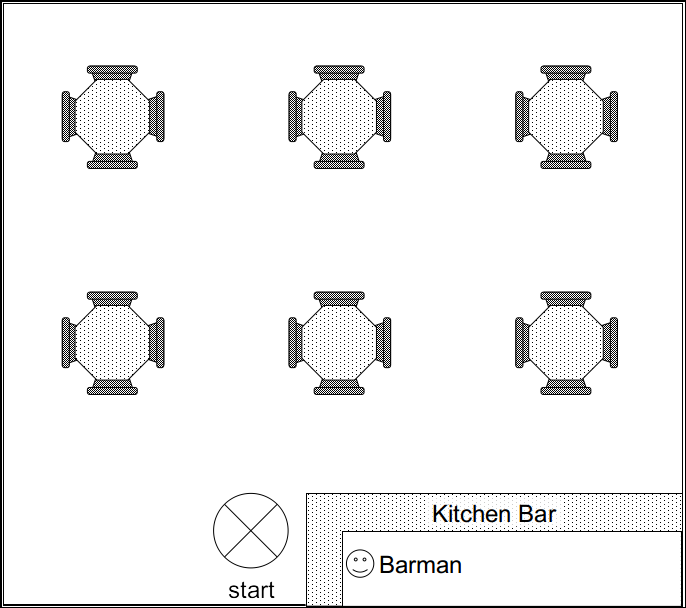
\includegraphics[width=0.5\columnwidth]{images/restaurant.png}
	\caption{Restaurant test: example setup.}
	\label{fig:restaurant}
\end{figure}

\subsection{Additional rules and remarks}

\begin{itemize}
	\item \textbf{Safety!} This test takes place in a public area. That is, there may be people standing, sitting or walking around the area throughout the test. The robot is expected to not even slightly touch anything and is immediately stopped in case of danger.

	\item \textbf{Referees and guidance:} For safety reasons, the referees in this test are TC members. One of the referees follows the robot and is always in reach of the emergency button.

	\item \textbf{Start:} There is no fixed start signal in this test.

	\item \textbf{Order:} The way the user provides information to the robot is up to the robot's team. A natural interaction is preferred.

	\item \textbf{Location:} This test can be arranged in any real restaurant or shopping mall. If this is not possible, the test can be conducted in an arbitrary room containing the appropriate locations. The only requirement is that this room is not part of the arena and that the teams do not know the room beforehand. The exact location, including the object and delivery locations, will be defined by the technical committee on site (and in corporation with the local organization).

	\item \textbf{Natural walking:} The operator has to walk \quotes{naturally}, i.e., move forward facing forward. If not mentioned otherwise, the operator is not allowed to walk back, stand still, signal the robot or follow some recalibration procedure.

	\item \textbf{Disturbances from outside:} If a person from the audience (severely) interferes with the robot in a way that makes it impossible to solve the task, the team may repeat the test immediately.

	\item \textbf{Learning tables:} Of course, it can only be sure that a robot correctly learned a table when it is able to go there after being commanded so. 
	
	\item \textbf{Instruction:} The robot interacts with the operators, not the team. That is, the team is only allowed to (very!) briefly instruct the \textit{Professional Waiter} and \textit{Professional Barman} 
	\begin{itemize}
		\item how to the tell the robot to follow,
		\item how to visually/acoustically indicate table names and position (e.g., pointing or telling \quotes{Table 1 is on your left}), 
		\item how to the tell the robot the \textit{Guide Phase} has ended, and
		\item how to the tell the robot the order has been served
	\end{itemize}
	It is not allowed to the team to instruct the clients on how to get robot's attention. It shall be done in a natural way like when interacting with a human waiter.

	\item \textbf{Kitchen-bar:} The \textit{Kitchen-bar} will be a table located at the restaurant's kitchen, next to the place where the \textit{Guide Phase} started and ended. 
	The robot may ask on which side of the robot the Kitchen-bar is, e.g. on its left or right side. It may ask this at the beginning or the end of the guide phase.
	It has the following setup.
	\begin{itemize}
		\item \textbf{Barman:} A \textit{Professional Barman} (member of the TC) will be at the other side of the Kitchen-bar to take the order provided by the robot and serve it in the official tray.
		\item \textbf{Beverages:} Beverages will be located on the Kitchen-bar next to the \textit{Professional Barman}.
	\end{itemize}

\end{itemize}

% \subsubsection{Referee instructions}

% The referee needs to
% \begin{itemize}
% \item 
% \item 
% \end{itemize}

% \subsubsection{OC instructions}

% \textbf{2 hours before the test}
% \begin{itemize}
% \item 
% \item 
% \end{itemize}
% \textbf{During the test}
% \begin{itemize}
% \item 
% \item 
% \end{itemize}

\newpage
\subsection{Score sheet}
The maximum time for this test is 15 minutes.

\small\begin{scorelist}

	\scoreheading{Training phase}
	\scoreitem[3]{10}{Learning the location of a table (Professional Waiter)}
	\scoreitem[3]{5}{Learning the location of a table (Custom Waiter)}
	\scoreitem[3]{10}{Inferring the side on which a table is (Professional Waiter only)}
	
	\scoreheading{Ordering phase}
	\scoreitem{5}{Understanding which table to take an order from}
	\scoreitem{15}{Going to the designated table}
	\scoreitem{10}{Taking an order from the designated table}
	\scoreitem{20}{Noticing a waving/calling person from distance}
	\scoreitem{20}{Going to the table of the waving/calling person}
	\scoreitem{10}{Taking an order from the waving/calling person}
	\scoreitem{10}{Avoiding a person crossing the robots' path}

	\scoreheading{Delivering phase}
	\scoreitem[2]{5}{Reciting both the order and table number for both tables}
	\scoreitem{10}{Grasping the correct drink}
	\scoreitem{15}{Getting close to the correct table with the drink}
	\scoreitem{15}{Delivering the drink by placing it on the correct table}
	\scoreitem{15}{Picking up the plate}
	\scoreitem{15}{Getting close to the correct table with the plate}
	\scoreitem{20}{Delivering the plate by placing it on the correct table}

	\setTotalScore{250}
\end{scorelist}



% Local Variables:
% TeX-master: "Rulebook"
% End:


% Local Variables:
% TeX-master: "Rulebook"
% End:


\newpage
%%%%%%%%%%%%%%%%%%%%%%%%%%%%%%%%%%%%%%%%%%%%%%%%%%%%%%%%%%%%%%%%%%%%%%%%%%%%%
%
% EEGPSR
%
%%%%%%%%%%%%%%%%%%%%%%%%%%%%%%%%%%%%%%%%%%%%%%%%%%%%%%%%%%%%%%%%%%%%%%%%%%%%%

% Number of concurrent teams
\newcommand{\eegpsrTeams}{2~}
% Maximum number of commands to be given to a robot
\newcommand{\eegpsrMaxCmd}{3~}
% Maximum amount of time given to a team to perform a single command
\newcommand{\eegpsrMaxCmdTime}{5~}
% Maximum amount of time given to a team to perform all commands
\newcommand{\eegpsrMaxTeamTime}{\eegpsrMaxCmd$\times$\eegpsrMaxCmdTime}

\section[EEGPSR]{E\textsuperscript{2}GPSR \\ \normalsize{(Enhanced Endurance General Purpose Service Robot)}}
\label{sec:eegpsr}

This test evaluates the required robot abilities throughout the Stage I \& II tests this (\YEAR) and previous years' rulebook. In EEGPSR the robot has to solve multiple tasks that are chosen randomly by the referees from a larger set of actions, over an extended period of time (30-45 minutes). In other words, tasks are not incorporated into a (predefined) story and there is neither a predefined order of tasks nor a predefined set of actions.
The actions to be carried out by the robot are organized in several categories with equivalent complexity but targeting different abilities.
It is upto the teams to choose how to execute the command and solving the involved tasks according to robot capabilities.
Scoring thereby depends on the complexity of the abilities shown.

\subsection{Focus}
This test particularly focuses on the following aspects:
\begin{itemize}
	\item No predefined order of actions to carry out.
	\item Increased complexity in speech recognition.
	\item More advanced capabilities
	\item Environmental (high-level) reasoning
	\item Robust long-term operation.

\end{itemize}

\subsection{Task}

\begin{enumerate}
	\item \textbf{Entering and command retrieval:} The robot enters the arena and drives to a designated position where it has to wait for further commands. \\

	\item \textbf{Command generation:} A command is generated randomly depending on the category chosen by the team (see below). All commands are composed by up to three actions that the robot has to show it has recognized. The robot may repeat the understood command and ask for confirmation. If it can't recognize the command correctly, it can also ask the speaker to repeat the whole command again.

	\begin{enumerate}
		\item \textbf{Category I:} The command is focused in \textbf{Advanced Manipulation}.

		\item \textbf{Category II:} The command is focused in \textbf{Advanced Object Recognition}.

		\item \textbf{Category III:} The robot gets a command focused in Human-Robot Interaction (\textbf{HRI}) that does not include all the necessary information to accomplish the task.

		\item \textbf{Category IV:} The command is focused in \textbf{Memory and Awareness}. This category can only be chosen after the team has successfully accomplished another command.

		\item \textbf{Category V:} The command is focused in \textbf{People Recognition} and \textbf{Navigation}.

		\item \textbf{Category VI:} The command is focused in \textbf{simple tasks} involving Manipulation, Object Recognition, and Person Recognition.

	\end{enumerate}

%	 \\

%	Each new generated command may require information from the previously given ones. Also, the difficulty of the new commands will be increased with respect of the previously generated ones. \\

	\item \textbf{Task assignment:} The robot is given a command by the operator and may directly start to work on the task assignment. If a robot is unable to perform a command, it should get back to the operator, and clearly state \textbf{why} it wasn't able to accomplish the task. \\

%	 \\

	\item \textbf{Task execution:} The robot must stop the execution of a task and return to its designated position within \eegpsrMaxCmdTime minutes. Otherwise the robot must be moved to its designated position immediately. If a restart is still available to the team, it can be restarted at the designated position. \\

	\item \textbf{Returning:} After accomplishing the assigned task, the robot has to move back to its designated position to wait and retrieve the next command (i.e., go back to 1. without the need of re-entering the arena). The robot can work on at most \eegpsrMaxCmd commands. \\

	\item \textbf{Timing:} The total time allotted to the robot for command retrieval and task execution is \eegpsrMaxTeamTime minutes. If the robot is not at its designated position after the time has expired, it must be moved at its designated position immediately. See the section on scheduling below as well.\\

	\item \textbf{Exiting the arena:} When commanded to do so, a robot should leave the arena. \\

\end{enumerate}

\subsection{Additional rules and remarks}
\label{sec:eegpsr-remarks}
\begin{enumerate}
	\item \textbf{CONTINUE rule:} Teams are able to use the CONTINUE rule in this test, with all the standard penalties it involves as described in section \refsec{rule:asrcontinue}.
	%The CONTINUE rule can only be used with the custom operator (e.g. both penalties of custom speaker and CONTINUE rule will be applied). 
	\\

	\item \textbf{Number of Teams and Scheduling:} In each test slot multiple teams (preferably \eegpsrTeams teams) may be competing in the arena concurrently. The robots will be tested in an interleaved fashion: The robots will retrieve commands and execute the task one after the other. As stated above, each robot will have a maximum amount of \eegpsrMaxCmdTime minutes per command (including time for retrieving the command and executing it). \\
	
	\item \textbf{Returning to designated position:} To facilitate a fluent and untroubled performance of the robots, they must return (or being returned) to their designated position before the \eegpsrMaxCmdTime minutes command time elapses. \textbf{If a robot moves from its designated position while another robot is working on a command, it must be immediately disabled} and moved to its designated position. If a restart is still available to the team, it can be restarted at its designated position. \\

	\item \textbf{Carrying robots:}	To carry the robot, at most two team members are allowed in the arena, and the robot must be moved as quickly as possible. To start or restart the robot, at most one team member may operate the robot. The team members moving and operating the robots must leave the arena immediately after the robot is placed or started. \\

	\item \textbf{Referees:} Since the score system in this test involves a subjective evaluation of the robot's behavior, the referees are EC/TC members. One referee is assigned to each team to judge performance, to measure the time for working on a command, and to keep track of the overall operating time of the robot. \\

	\item \textbf{Category selection:} For every of the three commands given to the robot, the team chooses the desired command category. Please do note that points for showing an ability can only be scored once, as also detailed in the next point.\\

	\item \textbf{Scoring:} Points are scored per ability with the total score of the test being the sum of the points scored in each successfully demonstrated ability while solving the tasks (see score sheet). Abilities will be scored considering the best execution only (e.g.~successfully grasping scores for \textit{grasping}), with the single exception of collision-free navigation. \\

	\item \textbf{Operator:}
	\begin{itemize}
		\item The person operating the robot is one of the referees (default operator).
		\item If the robot appears to consistently not be able to understand the operator, the referees ask the team to apply the CONTINUE rule (\refsec{rule:asrcontinue}).
	\end{itemize}

	\item \textbf{Inoperative robots:} If a robot gets stuck while trying to accomplish a task during a reasonable amount of time (e.g.~30 seconds), the referee may ask the team to move back the robot to its designated position, proceeding with the next robot. \\

	\item \textbf{Restart:} The number of commands to be given to a robot is three regardless if the restart were used or not. If a restart is required during before the first half of the total time allowed for execute a command elapses, a new command will be generated for the robot to perform. If the first half of the time has elapsed, the team may proceed with the restart but no new command will be generated and the robot must wait for the remaining commands (if any). Robots will be restarted at their designated position, \textbf{it won't be allowed to start outside the arena.} \\

	\item \textbf{Changing/Charging batteries:} The team may install a charging station at the designated position of the robot, if it does not hinder the other robots. However, the robot must connect itself with the charging station after carrying out a command. Changing batteries or manually connecting the robot with the charging station is allowed during a restart. \\

	\item \textbf{Scoring:} Robots are scored by successfully performed ability and full command completion within time. 
\end{enumerate}

\subsection{OC instructions}
\textbf{2h before test:}
\begin{itemize}
	\item Specify and announce the entrance/exit door for each robot. 
	\item Specify and announce the waiting position for each robot. 
\end{itemize}
\textbf{During the test:}
\begin{itemize}
	\item Help placing items and arranging people upon referee request.
\end{itemize}

\subsection{Referee instructions}
\textbf{During the test:}
\begin{itemize}
	\item Generate random sentences. %by an automatic sentence generator.
	\item Take the command and total time per team.
\end{itemize}


\newpage
\subsection{Score sheet}
\ifEvaluationSheet{

{\LARGE\textbf{Given commands:}}\vspace{4mm}

\newcommand{\eegpsrsstrow}{
	\multicolumn{6}{c}{\vspace{5mm}~}  \\ \hline
	\multicolumn{6}{c}{\vspace{5mm}~}  \\ \hline
	Category: 1 2 3 4 5 6 7 \vspace{8mm} &
%	Restart? & Custom Operator? & Continue? & ASR attempts: 1 2 3 \\
	{\footnotesize Restart?} & {\footnotesize Custom Operator?} & {\footnotesize MAN Bypass?} & {\footnotesize ASR Bypass?} & {\footnotesize ASR attempts:} $\Box \Box \Box$ \\
}

\begin{table}[h]
\begin{tabularx}{\textwidth}{X r r r r r}
	\textbf{\large Command 1:} & ~ & ~ & ~ & ~ & ~ \\ \hline
	\eegpsrsstrow

	\textbf{\large Command 1 $\cdot$ 2:} & ~ & ~ & ~ & ~ & ~ \\ \hline
	\eegpsrsstrow
	
	\textbf{\large Command 1 $\cdot$ 2 $\cdot$ 3 :} & ~ & ~ & ~ & ~ & ~ \\ \hline
	\eegpsrsstrow

	\textbf{\large Command 1 $\cdot$ 2 $\cdot$ 3 :} & ~ & ~ & ~ & ~ & ~ \\ \hline
	\eegpsrsstrow
\end{tabularx}
\end{table}
\vspace*{\fill}

\textbf{Remark: } Abilities marked with \textbf{*} are subjectively evaluated by  EC/TC members. Scoring is granted proportionally based on robot performance.

\newpage
}{}

The maximum time for this test is 40 minutes.

\begin{scorelist}
	\scoreheading{Performance}
	\scoreitem{15}{Understanding the command the $1^{st}$ attempt}
        \scoreitem{10}{Understanding the command the $2^{nd}$ attempt}
        \scoreitem{ 5}{Understanding the command the $3^{rd}$ attempt}
	\scoreitem{15}{Random category successfully solved}
	\scoreitem{20}{Mixing categories (bonus for each extra category)}
	
	\scoreheading{HRI}
	\scoreitem{ 5}{Answering a predefined question}
	\scoreitem{10}{Ask for missing information}
	\scoreitem{ 5}{Ask for command after detecting an event}
	\scoreitem{10}{Explain in detail why the robot could not accomplish a task *}
	\scoreitem{20}{Natural handover (give or take)}

	\scoreheading{Manipulation}
	\scoreitem{ 5}{Grab/place an object}
	\scoreitem{15}{Grab/place a stacked object}
	\scoreitem{30}{Manipulation in narrow spaces}
	\scoreitem{50}{Open/close a bottle/can *}
	\scoreitem{20}{Open/close a door/drawer *}
	\scoreitem{30}{Manipulation of buttons/levers/panels}
	\scoreitem{30}{Manipulation of tiny/heavy/slippery objects}
	\scoreitem{50}{Pour into a bowl *}
	\scoreitem{30}{Two-handed manipulation *}
	
	\scoreheading{Memory \& Awareness}
	\scoreitem{10}{Detect an expected event (within a reasonable amount of time) *}
	\scoreitem{20}{Detecting an unexpected event*}
	\scoreitem{20}{Provide information about changes in the environment and/or given commands*}

	\scoreheading{Navigation}
	\scoreitem{20}{Follow operator until stopped}
	\scoreitem{20}{Guide a human to location without loosing him or colliding}
	
	\scoreheading{Object recognition}
	\scoreitem{10}{Counting overall objects}
	\scoreitem{30}{Counting objects in category}
	\scoreitem{50}{Counting objects matching description *}
	\scoreitem{30}{Describing an unknown object}
	\scoreitem{30}{Find (and grasp) an object from a description *}
	\scoreitem{30}{Find occluded object (>50\% occlusion)}
	\scoreitem{50}{Find hidden object (100\% occlusion)}
	\scoreitem{50}{Infer unknown object's class (category) from features}
	\scoreitem{15}{Recognize alike object}
	\scoreitem{ 5}{Recognize known object}

	\scoreheading{People, pose and activity recognition}
	\scoreitem{15}{Detect a calling/waving person}
	\scoreitem{15}{Find a person in a given room}
	\scoreitem{15}{Recognize a newly learned face correctly}
	\scoreitem{20}{State the gender of a person}
	\scoreitem{15}{State the number of people in a group}
	\scoreitem{20}{State the pose of a person *}

	\setTotalScore{0}
\end{scorelist}


% Local Variables:
% TeX-master: "Rulebook"
% End:


% Local Variables:
% TeX-master: "Rulebook"
% End:
 


\newpage
\chapter{Finals}

The competition ends with the Finals on the last day, where the five teams with the highest total score compete. The \iterm{Finals} are conducted as a final open demonstration where the robots show their best abilities. This demonstration does not have to be different from the other open demonstration ---open challenge--- nor have to be the same either.

\section{Final Demonstration}

In the final demonstration, every team qualified for the finals can choose freely what to demonstrate. The demonstration is evaluated by both a league-internal and a league-external jury, considering also the score during the competition.

It is intended to show that a robot is able to perform a set of advanced skills integrated into a simple story driven at home. The story, in which the robot is the main character, must be easy to understand and self explicative.

\subsection{Task}
The procedure for the demonstration and the timing of slots is as follows:
\begin{enumerate}
  \item \textbf{Setup and demonstration:} The team has a maximum of ten minutes for setup and demonstration. During the demonstration, the robot must perform at least 2 complex tasks from different categories (see \refsec{chap:example-skills}for a list of examples on each category) to be evaluated by the League-internal jury. During Setup Time and before the demonstration begins, the team leader is allowed to \emph{very} briefly describe the story (maximum time is one minute). \\
  \item \textbf{Interview and cleanup:} After the demonstration, there is another five minutes where the team answers questions by the jury members. The team may prepare one slide with technical information of the task to rely on during the interview in case that projectors are available.

  During the interview time, the team has to undo its changes to the environment.
\end{enumerate}

\subsection{Evaluation and Score System}
The demonstration is evaluated by both a league-internal and a league-external jury. The final score and ranking are determined by the two jury evaluations and by the previous performance (in Stages I and II) of the team.

\begin{enumerate}
  \item \textbf{League-internal jury:} The league-internal jury is formed by the Executive Committee.
  The evaluation of the league-internal jury is based on the following criteria:
  \begin{enumerate}
    % \item Novelty (Seen before in @Home?)
    \item Scientific contribution (Is that new in @Home?)
    \item Performance executing complex skill 1
    \item Performance executing complex skill 2
    \item Contribution for @Home (can other teams use the solution?)
    \item Performance executing each additional complex skills (if any, scoring as bonus)

  % MAURICIO: Previous evaluation criteria (2014)
  %  \item Scientific contribution
  %  \item Contribution to @Home
  %  \item Relevance for @Home / Novelty of approaches
  %  \item Presentation and performance in the finals.
  \end{enumerate}
  It is expected that teams present their scientific and technical contributions in
  % MAURICIO: I removed the wiki
  % both team description paper and the RoboCup@Home Wiki.
  the team description paper .
  In addition, finalist teams may provide a printed document to the jury (max 2 pages) that summarizes the demonstrated robot capabilities and contributions.

  The influence of the league-internal jury to the final ranking is 25\%. \\

  \item \textbf{League-external jury:} The league-external jury consists of people not being involved in the RoboCup@Home league, but having a related background (not necessarily robotics). They are appointed by the Executive Committee. The evaluation of the league-external jury is based on the following criteria:
  \begin{enumerate}
    \item Integration of skills in story (story-telling is to be rewarded)
    \item Difficulty of the performance (How difficult is it?)
    \item Success of the performance (The robot did it?)
    \item System integration (How smooth was the execution?)
    \item Relevance / Usefulness for daily life (I want that robot in my home!)
  % MAURICIO: Previous evaluation criteria (2014)
  %  \item Originality and Presentation (story-telling is to be rewarded)
  %  \item Usability / Human-robot interaction
  %  \item Multi-modality / System integration
  %  \item Difficulty and success of the performance
  %  \item Relevance / Usefulness for daily life
  \end{enumerate}

  The influence of the league-external jury to the final ranking is 25\%. \\

  \item \textbf{Previous performance:} 50\% of the final score are determined by the team's previous performance during the competition, i.e., the sum of points scored in Stage I and Stage II.
\end{enumerate}

\subsection{Changes to the environment}
\begin{enumerate}
  \item Making changes: As in the other open demonstrations, teams are allowed to make modifications to the arena as they like, but under the condition that they are reversible.
  \item Undoing changes: In the interview and cleanup team, changes need to be made undone by the team. The team has to leave the arena in the very same condition they entered it.
\end{enumerate}

\subsection{Final Ranking and Winner}
The winner of the competition is the team that gets the highest ranking in the finals

There will be an award for 1st, 2nd and 3rd place. All teams in the Finals receive a certificate stating that they made it into the Finals of the RoboCup@Home competition.


% Local Variables:
% TeX-master: "Rulebook"
% End:


\begin{appendices}
% \addto\captionsenglish{\renewcommand{\chaptername}{Appendix}}
% \renewcommand{\chaptername}{Appendix}
\renewcommand*{\chapterformat}{\LARGE{Appendix \thechapter}}
\renewcommand{\chaptermark}[1]{\markboth{\appendixname \ \thechapter. \ #1}{}}

\chapter{Robo-Nurse diseases and symptoms list}

The following section presents the list of diseases an their symptoms to be used during the \textit{Robo-Nurse test}. Note that the list of symptoms is not extensive nor has been normalized in order to allow the teams to perform their own research on medical diagnosis.

\section{Disease list (by alphabetic order)}

\begin{itemize}

\item \textbf{Acid reflux:} Heartburn (acid indigestion), regurgitation (wet burp), burping, nausea after eating, stomach fullness or bloating, upper abdominal pain and discomfort. Treatment: anti-acid.

\item \textbf{Anemia:} Easy fatigue and loss of energy, unusually rapid heart beat (particularly with exercise), shortness of breath and headache (particularly with exercise), difficulty concentrating, dizziness, pale skin, leg cramps, insomnia, hunger for strange substances such as paper, ice, or dirt (a condition called pica); upward curvature of the nails (referred to as koilonychias), soreness of the mouth with cracks at the corners; tingling, \quotes{pins and needles} sensation in the hands or feet; lost sense of touch, a wobbly gait and difficulty walking, clumsiness and stiffness of the arms and legs. Treatment: take alimentary supplements, rest.

\item \textbf{Arthritis:} At the joint: pain, stiffness, swelling, redness, decreased range of motion. Treatment: medical advice, ice, pain killers.

\item \textbf{Back Pain:} Persistent aching or stiffness anywhere along your spine (from the base of the neck to the tail bone), sharp, localized pain in the neck, upper back, or lower back (especially after lifting heavy objects or engaging in other strenuous activity); chronic ache in the middle or lower back, especially after sitting or standing for extended periods; back pain that radiates from the low back to the buttock, down the back of the thigh, and into the calf and toes; inability to stand straight without having pain or muscle spasms in the lower back. Treatment: medical advice, pain killers.

\item \textbf{Common Cold:} Runny or stuffy nose, itchy or sore throat, cough, congestion, slight body aches, sneezing, watery eyes, low-grade fever, mild fatigue. Treatment: water, rest, chicken soup.

\item \textbf{Dandruff:} Flakes of skin on the scalp and hair (from small and white to large, greasy and yellow), head may feel tight and itchy, head may feel tingly, head may feel sore, red, flaky, greasy patches of skin. Special shampoo.

\item \textbf{Dehydration:} Dry and sticky mouth, sleepiness or tiredness, thirst, decreased urine output, few or no tears when crying, dry skin, headache, constipation, dizziness or lightheadedness. Treatment: water.

\item \textbf{Diarrhea:} Frequent, loose, watery stools; abdominal cramps, abdominal pain, fever, blood in the stool, bloating. Treatment: water, steamed vegetables, a cork.

\item \textbf{Flu:} Severe aches in joints and muscles, pain and tiredness around eyes, weakness or fatigue, warm, flushed skin and red, watery eyes; headache, dry cough, sore throat and runny nose. Treatment: water, rest, antiviral drug (Tamiflu).

\item \textbf{Headache: } Caused by alcohol (particularly red wine) certain foods (such as processed meats that contain nitrates, berries and nuts), changes in sleep or lack of sleep, poor posture, skipped meals, stress. Treatment: rest, aspirin, pain-killers.

\item \textbf{Heartburn:} Caused by strong drinks (alcohol, caffeine, carbonated water), acidic juices (grapefruit, orange, pineapple), drugs (aspirin, ibuprofen, Naproxen), acidic foods (tomatoes, grapefruit, oranges), fat-rich food (meat, chocolate), and smoking. Treatment: anti-acid.

\item \textbf{Heat Stroke:} Core body temperature above 105°F/45.5°C (Hallmark symptom), throbbing headache, dizziness and light-headedness, lack of sweating despite the heat, red, hot, and dry skin; muscle weakness or cramps, nausea and vomiting, rapid heartbeat, which may be either strong or weak; rapid, shallow breathing; behavioral changes such as confusion, disorientation, or staggering; seizures, unconsciousness. Treatment: Fan air over the patient's wet body, apply ice packs to the patient's armpits, groin, neck, and back, immerse the patient in a shower or tub of cool water, or an ice bath. Call ambulance.

\item \textbf{Hyperglycemia (high blood sugar):} Frequent urination, increased thirst,
blurred vision, fatigue, fruity-smelling breath, nausea and vomiting, shortness of breath, dry mouth, weakness, confusion, abdominal pain, headache. Treatment: medical assistance required, call for ambulance.

\item \textbf{Hypertension (high blood pressure):} Severe headache fatigue or confusion, vision problems, chest pain, difficulty breathing, irregular heartbeat, blood in the urine, pounding in your chest, neck, or ears. Treatment: medical assistance required, call for ambulance.

\item \textbf{Hypoglycemia (low blood sugar):} Sweating (almost always present, check for sweating on the back of neck at your hairline), nervousness, shakiness, and weakness; extreme hunger and slight nausea, dizziness and headache, blurred vision, a fast heartbeat and feeling anxious. Treatment: food.

\item \textbf{Hypotension (low blood pressure):} Dizziness or lightheadedness, unsteadiness, fainting (syncope), lack of concentration, dimming or blurred vision, nausea; cold, clammy skin; pale skin; rapid or shallow breathing, fatigue depression, thirst, weaknTuberculosisess.

\item \textbf{Migraine:} One day or two before: depressed or cranky, very happy, very awake, or full of energy; restless or nervous, very sleepy, thirsty or hungry, or may crave certain foods, or may not feel like eating. 30 minutes before: See spots, wavy lines, or flashing lights; have numbness or a \quotes{pins-and-needles} feeling in hands, arms, or face. Once it's started: Throbbing pain on one side (or even both sides) of the head, pain behind one of the eyes, moderate to very bad pain (it may be so bad that can't perform any of the usual activities), pain that gets worse with routine physical activity, nausea, vomiting, or both; pain that gets worse when around light, noise, and sometimes smells. Treatment: Pain-killers.

\item \textbf{Pharyngitis:} Red throat, sore throat, runny or stuffy nose, dry cough, hoarseness, redness of the eyes, fever, headache, joint pain and muscle aches, skin rashes, swollen lymph nodes (glands) in the neck, body ache and a general sick feeling generally sick feeling. Treatment: rest, ibuprofen, warm liquids, medical advice to get antiviral or antibiotic treatment.

\item \textbf{Pneumonia:} Cough (often producing mucus, also called sputum, from the lungs), mucus may be rusty or green or tinged with blood, fever (which may be less common in older adults), Shaking, \quotes{teeth-chattering} chills, fast, often shallow, breathing and the feeling of being short of breath; chest wall pain that is often made worse by coughing or breathing in, fast heartbeat, feeling very tired or weak, nausea and vomiting, shortness of breath, little mucus when coughing, diarrhea.Treatment: rest, ibuprofen, warm liquids. Medical assistance required.

\item \textbf{Premenstrual syndrome:} Tension or anxiety, sad or depressed mood, crying spells, mood swings and irritability or aggression or anger; appetite changes and food cravings, insomnia, social withdrawal, poor concentration, joint or muscle pain, headache, fatigue, weight gain related to fluid retention, abdominal bloating, breast tenderness, acne flare-ups, constipation or diarrhea. Treatment: ibuprofen, antispasmodic, warm liquids.

\item \textbf{Ringworm: }. On the scalp: dry, brittle hair or hair loss in patches; severe itching, red-ringed patch of small blisters or scaly skin. On the body: red-ringed patch of small blisters or scaly skin, severe itching is sometimes present Treatment: Apply ice to reduce itching and call medic to get prescriptive medicine.

\item \textbf{Scabies:} Intense itching (especially at night), a pimple-like rash, scales or blisters, sores caused by scratching. Treatment: Call medic to get prescriptive medicine. Take antihistamine pills and apply hydrocortisone cream after medical diagnosis.

\item \textbf{Sinusitis:} Pain and pressure in the face along with a stuffy or runny nose (main symptoms), yellow or greenish discharge from nose, headache, yellow or greenish discharge from the nose or down the back of the throat, bad breath, stuffy nose, cough that produces mucus, fever, tooth pain, reduced sense of taste or smell.Treatment: Drink plenty of fluids, apply moist heat (using a hot, damp towel or gel pack) for 5 to 10 minutes, breathe warm, moist air (from a steamy shower, a hot bath, or a sink filled with hot water).

\item \textbf{Sunburn:} Skin turns red and hurts, swelling and sunburn blisters (sever burn) feel like you have the flu (feverish, with chills, nausea, headache, and weakness). Treatment: Drink plenty of water, apply cold compresses , take nonsteroidal anti-inflammatory drugs, like ibuprofen or Naproxen, gently rub on a cream or gel containing menthol, camphor or aloe.

\item \textbf{Sun Poisoning:} Skin redness and blistering, pain and tingling, swelling, headache, fever and chills, nausea, dizziness, dehydration. Treatment: Get out of the sun, take a cool (not cold) shower or bath or apply cool compresses, drink extra fluids for a few days, take ibuprofen or acetaminophen to relieve pain, use aloe gel or a moisturizer, completely cover sunburned areas when going outside.

\item \textbf{Tuberculosis:} Coughing that lasts three o symptoms more weeks, coughing up blood, chest pain, or pain with breathing or coughing; unintentional weight loss, fatigue, fever, night sweats, chills, loss of appetite. Treatment: Drink plenty of fluids, eat healthy food. Quarantine: medical assistance required, call for ambulance.

\item \textbf{Urticaria:} Swollen, pale red bumps or plaques (wheals) on the skin, itching, burning or stinging. Treatment: Apply cool compresses or wet cloths to the affected areas, antihistamine.

\end{itemize}


% Local Variables:
% TeX-master: "Rulebook"
% End:


\chapter{Example Skills}
\label{chap:example-skills}

The following section presents a list of \iterm{Example Skills} with an high degree of difficulty which can be exploited during the \textit{Open Demonstrations} (See \refsec{sec:open-demonstrations}.
Other skills not on this list (yet) may be added as well. If you want to do so, please let the TC know via email (tc@robocupathome.org) for their inclusion on the RuleBook so all teams may also show this skill.

Please note that these examples are to illustrate the level of complexity and applicability that should be shown. For instance, \quotes{Handle a pan} is listed in the category of \textit{Complex manipulation}, but it is extensive to handling pans, pots, woks and any other cookware with handles.

\section{Skills by category}

\subsection{Complex manipulation}
\begin{itemize}
	\item Cook a meal.
	\item Manipulating panels/switches/knobs.
	\item Use/open a fridge/stove/blender/microwave/washing machine.
	\item Iron clothes.
	\item Move a movable object (pole, chair, table).
	\item Pouring liquids/powders.
	\item Operate a water tap.
	\item Handle a pan.
\end{itemize}

\subsection{Complex vision}
\begin{itemize}
	\item Read text from a newspaper.
	\item Handle glass/shiny-metallic objects.
	\item Recognize moods, activities, age, gender.
%	\item Recognize clothes, dressing-styles, fashionable people.
	\item Label unknown objects.
\end{itemize}

\subsection{Complex navigation}
\begin{itemize}
	\item Navigate in (very) crowded environments.
	\item Navigate difficult terrain.
	\item Climb stairs.
	\item Push a wheelchair.
\end{itemize}

\subsection{Robot-Human Interaction}
\begin{itemize}
	\item Collaborative robot-human manipulation.
	\item Maintaining a conversation.
	\item Learning actions on-the-fly.
	\item Learning objects from humans e.g. ``This object is a ...'' with an open vocubulary.
	\item Following a human by grasping its hand.
	\item Explain the robot abstract concepts (why people love sunny days).
	\item Arrange unknown random people for a nice photo (no occlusions).
	% \item ask the robot for the answer to the universe, meaning of life and everything else
\end{itemize}

\subsection{Complex action planning} 
\begin{itemize}
	\item Separate clothes for laundry (e.g.~by color)
	\item Arrange a dish-washer.
	\item Take a cup from the cupboard whose location has changed, is closed, or the path to it is blocked (e.g.~by a chair).
	\item Light the way out with a lamp during a general power off.
	\item Arrange unknown random people for a nice photo (no occlusions).
	\item 
\end{itemize}

\subsection{Mapping}
\begin{itemize}
	\item Learn/create a (3D) map on the fly.
	\item Semantically annotate a map on the fly
	\item The robot enters a completely changed arena (furniture moved or even changed), 
	   explores it and is told to go to e.g. a table that is moved or added.
\end{itemize}


% Local Variables:
% TeX-master: "Rulebook"
% End:


\end{appendices}

% \renewcommand{\chaptername}{Chapter}
% \addto\captionsenglish{\renewcommand{\chaptername}{Chapter}}
\renewcommand*{\chapterformat}{\LARGE{Chapter \thechapter}}
\renewcommand{\chaptermark}[1]{\markboth{\chaptername \ \thechapter. \ #1}{}}


\printabx
\printidx

\end{document}
